% vim: set tw=80:spell
%
\documentclass[twoside,a5paper,10pt]{extarticle}
%\documentclass[twoside,14pt,draft]{extarticle}
%\documentclass[twoside,14pt,draft]{scrartcl}
\usepackage{amsmath}
\usepackage{amssymb}
\usepackage{amsfonts}
\usepackage{mathtext}
\usepackage{pdfpages}
\usepackage{parallel}
\usepackage[T2A]{fontenc}
\usepackage{ucs}
\usepackage[utf8x]{inputenc}
\usepackage[polish,english,russian]{babel}
\usepackage{hyperref}
\usepackage{rotating}
\usepackage[inner=2cm,top=1.8cm,outer=2cm,bottom=2.3cm,nohead]{geometry}
\usepackage{listings}
\usepackage{graphicx}
\usepackage{wrapfig}
\usepackage{longtable}
\usepackage{indentfirst}
\usepackage{array}
\newcolumntype{P}[1]{>{\raggedright\arraybackslash}p{#1}}
\frenchspacing
\usepackage{fixltx2e} %text sub- and superscripts
\usepackage{icomma} % коскі ў матэматычным рэжыме
\PreloadUnicodePage{4}

\newcommand{\longpage}{\enlargethispage{\baselineskip}}
\newcommand{\shortpage}{\enlargethispage{-\baselineskip}}

\def\switchlang#1{\expandafter\csname switchlang#1\endcsname}
\def\switchlangbe{
\let\saverefname=\refname%
\def\refname{Літаратура}%
\def\figurename{Іл.}%
}
\def\switchlangen{
\let\saverefname=\refname%
\def\refname{References}%
\def\figurename{Fig.}%
}
\def\switchlangru{
\let\saverefname=\refname%
\let\savefigurename=\figurename%
\def\refname{Литература}%
\def\figurename{Рис.}%
}

\hyphenation{admi-ni-stra-tive}
\hyphenation{ex-pe-ri-ence}
\hyphenation{fle-xi-bi-li-ty}
\hyphenation{Py-thon}
\hyphenation{ma-the-ma-ti-cal}
\hyphenation{re-ported}
\hyphenation{imp-le-menta-tions}
\hyphenation{pro-vides}
\hyphenation{en-gi-neering}
\hyphenation{com-pa-ti-bi-li-ty}
\hyphenation{im-pos-sible}
\hyphenation{desk-top}
\hyphenation{elec-tro-nic}
\hyphenation{com-pa-ny}
\hyphenation{de-ve-lop-ment}
\hyphenation{de-ve-loping}
\hyphenation{de-ve-lop}
\hyphenation{da-ta-ba-se}
\hyphenation{plat-forms}
\hyphenation{or-ga-ni-za-tion}
\hyphenation{pro-gramming}
\hyphenation{in-stru-ments}
\hyphenation{Li-nux}
\hyphenation{sour-ce}
\hyphenation{en-vi-ron-ment}
\hyphenation{Te-le-pathy}
\hyphenation{Li-nux-ov-ka}
\hyphenation{Open-BSD}
\hyphenation{Free-BSD}
\hyphenation{men-ti-on-ed}
\hyphenation{app-li-ca-tion}

\def\progref!#1!{\texttt{#1}}
\renewcommand{\arraystretch}{2} %Іначай формулы ў матрыцы зліпаюцца з лініямі
\usepackage{array}

\def\interview #1 (#2), #3, #4, #5\par{

\section[#1, #3, #4]{#1 -- #3, #4}
\def\qname{LVEE}
\def\aname{#1}
\def\q ##1\par{{\noindent \bf \qname: ##1 }\par}
\def\a{{\noindent \bf \aname: } \def\qname{L}\def\aname{#2}}
}

\def\interview* #1 (#2), #3, #4, #5\par{

\section*{#1\\{\small\rm #3, #4. #5}}

\def\qname{LVEE}
\def\aname{#1}
\def\q ##1\par{{\noindent \bf \qname: ##1 }\par}
\def\a{{\noindent \bf \aname: } \def\qname{L}\def\aname{#2}}
}

%\usepackage{portland}
%\usepackage{lscape}
%\usepackage{rotating}
\usepackage[labelsep=period,justification=centering]{caption}
%\usepackage{ccaption}
%\captiondelim{. }
\usepackage{hyphenat}
\usepackage{tweaklist}
\usepackage{pdfpages}
\usepackage{parallel}
%\usepackage{trace}
%\usepackage{tikz}
%\usetikzlibrary{calc}
%\usetikzlibrary{positioning}
\usepackage{subfig}
\renewcommand{\enumhook}{\setlength{\topsep}{0pt}%
  \setlength{\itemsep}{0pt}\setlength{\parskip}{0pt plus 1pt minus 1pt}\setlength{\parsep}{0pt}}
\renewcommand{\itemhook}{\setlength{\topsep}{0pt}%
  \setlength{\itemsep}{0pt}\setlength{\parskip}{0pt plus 1pt minus 1pt}\setlength{\parsep}{0pt}}
%\renewcommand{\enumhook}{\setlength{\topsep}{0pt}%
%  \setlength{\itemsep}{0pt}}
%\renewcommand{\itemhook}{\setlength{\topsep}{0pt}%
%  \setlength{\itemsep}{0pt}\setlength{\parskip}{0pt}\setlength{\parsep}{0pt}}
%\renewcommand{\enumhook}{\setlength{\topsep}{0pt}%
%  \setlength{\itemsep}{0pt}}
%\renewcommand{\itemhook}{\setlength{\topsep}{0pt}%
%  \setlength{\itemsep}{0pt}\setlength{\parsep}{0pt}}

\clubpenalty=10000%
\widowpenalty=10000%
%\setlength{\parindent}{1.25cm}%

\newcommand\familyname[1]{\textbf{#1}}

\DeclareMathOperator{\e}{e}
\DeclareMathOperator{\cov}{cov}
\DeclareMathOperator{\diag}{diag}

\newcommand\eof{\writetotalpages\end{document}\endinput}

\newcommand\key[1]{\textbf{#1}}
\newcommand\vect[1]{\mathbf{#1}}
\def\eqn #1 $#2${\begin{equation}\label{eq:#1}#2\end{equation}}
%\def\where #1
\newcommand\eqnref[1]{(\ref{eq:#1})}
\makeatletter
\def\p@subfigure{\thefigure,~}
\def\thesubfigure{\asbuk{subfigure}}
\newcounter{articleno}
\setcounter{articleno}0
\@newctr{figure}[articleno]
\renewcommand \thefigure {\@arabic\c@articleno.\@arabic\c@figure}
\@newctr{equation}[articleno]
\renewcommand\theequation{\@arabic\c@articleno.\@arabic\c@equation}
\newcommand\ps@twoside{%
 \makeatletter%
 \renewcommand\@oddfoot{~\hfill\thepage}%
 \renewcommand\@evenfoot{\thepage\hfill~}%
 \makeatother%
}
\newcounter{totalpages}
\def\writetotalpages{%
  \protected@write\@auxout
      {}%
      {\string\setcounter{totalpages}{\thepage}}}
\newcounter{totalfigures}%
\newcounter{totalsubfigures}%
\newcounter{totalsections}%
\newcounter{totalsubsections}%
\newcounter{totalsubsubsections}%
\newcounter{totalparagraphs}%

%\def\addcontentsline#1#2#3{%
%  \addtocontents{#1}{\protect\contentsline{#2}{#3}{\thepage}%
%  \protect\stepcounter{total#2s}}}
\makeatother
\newcommand\comment[1]{\textsf{#1}}
\renewcommand\labelitemi{\textendash}
\renewcommand\labelitemii{\textendash}


% перенос формул в тексте
\newcommand*{\hm}[1]{#1\nobreak\discretionary{}%
  {\hbox{$\mathsurround=0pt #1$}}{}}

\def\layersep{2.5cm}

\begin{document}
\switchlang{ru}
\addtocounter{page}{2}%
\pagestyle{twoside}

\makeatletter
\def\@starttoc#1{%
  \begingroup
    \raggedright
    \sloppy
    \makeatletter
    \@input{\jobname.#1}%
    \if@filesw
      \expandafter\newwrite\csname tf@#1\endcsname
      \immediate\openout \csname tf@#1\endcsname \jobname.#1\relax
    \fi
    \@nobreakfalse
    \fussy
  \endgroup}
\makeatother


\thispagestyle{empty}
\newpage
\tableofcontents

\def\documentclass[#1]#2{}

\makeatletter

\def\@self@name{00}
\def\@preamble@name{preamble.tex}

\def\document{\newpage}
\let\@lvee@enddoc\enddocument

\let\@lvee@input\input
\def\enddocument{%
\gdef\@title{}%
\gdef\@author{}%
}

\def\@lbibitem[#1]#2{\setlength{\topsep}{0pt}%
  \setlength{\itemsep}{0pt}\setlength{\parskip}{0pt plus 1pt minus 1pt}\setlength{\parsep}{0pt}%
    \item[\@biblabel{#1}\hfill]\if@filesw
      {\let\protect\noexpand
       \immediate
       \write\@auxout{\string\bibcite{#2}{#1}}}\fi\ignorespaces}
\def\@bibitem#1{\setlength{\topsep}{0pt}%
  \setlength{\itemsep}{0pt}\setlength{\parskip}{0pt plus 1pt minus 1pt}\setlength{\parsep}{0pt}%
    \item\if@filesw \immediate\write\@auxout
       {\string\bibcite{#1}{\the\value{\@listctr}}}\fi\ignorespaces}

\renewcommand\maketitle{\par
  \begingroup
     \def\@thanks{}% flush all the thanks we have already collected so they don't accumulate
     \renewcommand\thefootnote{\@fnsymbol\c@footnote}%
     \def\@makefnmark{\rlap{\@textsuperscript{\normalfont\@thefnmark}}}%
     \long\def\@makefntext##1{\parindent 1em\noindent
             \hb@xt@1.8em{%
                 \hss\@textsuperscript{\normalfont\@thefnmark}}##1}%
%     \if@twocolumn
%       \ifnum \col@number=\@ne
%         \@maketitle
%       \else
%         \twocolumn[\@maketitle]%
%       \fi
%     \else
      \newpage
      \global\@topnum\z@   % Prevents figures from going at top of page.
      \stepcounter{articleno}%
      \def\footnote##1{}
      \ifx \@author \@empty
          \addcontentsline{toc}{section}{\nohyphens{\@title}}%
      \else
          \addcontentsline{toc}{section}{\nohyphens{\@author: \@title}}%
      \fi
      \@maketitle
%     \fi
    \thispagestyle{twoside}\@thanks
  \endgroup
  \setcounter{footnote}{0}%
}

\def\@maketitle{%
  \newpage
  \null
  \begin{center}%
  \let \footnote \thanks
    {\LARGE \@title }\\%
    \ifx \@author \@empty
    \else
    {\large
      \lineskip .2em%
      \begin{tabular}[t]{c}%
        \@author
      \end{tabular}}%
    \fi
  \end{center}%
  \par
}

\def\input#1{
\let\@@@@curfile\@@@curfile
\def\@@@curfile{#1}
\message{@@\@@@curfile @@}
\ifx \@@@curfile \@preamble@name
    \message{An attempt to include the preamble has occured, ignoring.^^J}
\else
    \ifx \@@@curfile \@self@name
        \message{An attempt to include ourselves had occured, ignoring.^^J}
    \else
        \@lvee@input#1
    \fi
\fi
\let\@@@curfile\@@@@curfile
\message{ONEXIT @@\@@@curfile @@}
}

\def\abstract{%
        \small%
        \quotation \noindent}

\def\nocite#1{}
\def\bibliography#1{
    \makeatletter%
    \@lvee@input{\@@@curfile.bbl}
    \makeatother%
}

\makeatother 
\documentclass[10pt, a5paper]{article}
\usepackage{pdfpages}
\usepackage{parallel}
\usepackage[T2A]{fontenc}
\usepackage{ucs}
\usepackage[utf8x]{inputenc}
\usepackage[polish,english,russian]{babel}
\usepackage{hyperref}
\usepackage{rotating}
\usepackage[inner=2cm,top=1.8cm,outer=2cm,bottom=2.3cm,nohead]{geometry}
\usepackage{listings}
\usepackage{graphicx}
\usepackage{wrapfig}
\usepackage{longtable}
\usepackage{indentfirst}
\usepackage{array}
\newcolumntype{P}[1]{>{\raggedright\arraybackslash}p{#1}}
\frenchspacing
\usepackage{fixltx2e} %text sub- and superscripts
\usepackage{icomma} % коскі ў матэматычным рэжыме
\PreloadUnicodePage{4}

\newcommand{\longpage}{\enlargethispage{\baselineskip}}
\newcommand{\shortpage}{\enlargethispage{-\baselineskip}}

\def\switchlang#1{\expandafter\csname switchlang#1\endcsname}
\def\switchlangbe{
\let\saverefname=\refname%
\def\refname{Літаратура}%
\def\figurename{Іл.}%
}
\def\switchlangen{
\let\saverefname=\refname%
\def\refname{References}%
\def\figurename{Fig.}%
}
\def\switchlangru{
\let\saverefname=\refname%
\let\savefigurename=\figurename%
\def\refname{Литература}%
\def\figurename{Рис.}%
}

\hyphenation{admi-ni-stra-tive}
\hyphenation{ex-pe-ri-ence}
\hyphenation{fle-xi-bi-li-ty}
\hyphenation{Py-thon}
\hyphenation{ma-the-ma-ti-cal}
\hyphenation{re-ported}
\hyphenation{imp-le-menta-tions}
\hyphenation{pro-vides}
\hyphenation{en-gi-neering}
\hyphenation{com-pa-ti-bi-li-ty}
\hyphenation{im-pos-sible}
\hyphenation{desk-top}
\hyphenation{elec-tro-nic}
\hyphenation{com-pa-ny}
\hyphenation{de-ve-lop-ment}
\hyphenation{de-ve-loping}
\hyphenation{de-ve-lop}
\hyphenation{da-ta-ba-se}
\hyphenation{plat-forms}
\hyphenation{or-ga-ni-za-tion}
\hyphenation{pro-gramming}
\hyphenation{in-stru-ments}
\hyphenation{Li-nux}
\hyphenation{sour-ce}
\hyphenation{en-vi-ron-ment}
\hyphenation{Te-le-pathy}
\hyphenation{Li-nux-ov-ka}
\hyphenation{Open-BSD}
\hyphenation{Free-BSD}
\hyphenation{men-ti-on-ed}
\hyphenation{app-li-ca-tion}

\def\progref!#1!{\texttt{#1}}
\renewcommand{\arraystretch}{2} %Іначай формулы ў матрыцы зліпаюцца з лініямі
\usepackage{array}

\def\interview #1 (#2), #3, #4, #5\par{

\section[#1, #3, #4]{#1 -- #3, #4}
\def\qname{LVEE}
\def\aname{#1}
\def\q ##1\par{{\noindent \bf \qname: ##1 }\par}
\def\a{{\noindent \bf \aname: } \def\qname{L}\def\aname{#2}}
}

\def\interview* #1 (#2), #3, #4, #5\par{

\section*{#1\\{\small\rm #3, #4. #5}}

\def\qname{LVEE}
\def\aname{#1}
\def\q ##1\par{{\noindent \bf \qname: ##1 }\par}
\def\a{{\noindent \bf \aname: } \def\qname{L}\def\aname{#2}}
}

\begin{document}
\title{Многослойные и многоуровневые системы хранения данных.\footnote{\url{alex_kls@mail.ru} \url{http://lvee.org/ru/abstracts/238}}}
\author{Александр Клыга, Minsk, Belarus}
\maketitle
\begin{abstract}
In multilayers data storages the storage drivers are grouped into
separate layers according to their technical characteristics. The first layer contains high-speed solid-state drivers (SSDs), whereas the other layers can have HDDs or others storage devices (tape, optical devices). The multilayer data storage provides high speed data access and can be formed by using hardware or software solutions. In multilevel software-define storages (SDS), the separate data storage are grouped with respect to levels of their technical characteristics, the type of stored data, and availability requirements for the end user. Multilevels SDS allows for optimization of the data placement in the storage. The main node of SDS is represented by a controller. The SDS controller is a software platform (open source and other) which includes solution tools for management, monitoring and migration of data between layers.
\end{abstract}
\subsection*{Многослойные и многоуровневые системы хранения данных. Обзор архитектуры и решений на базе open source.}

В настоящее время развитие систем хранения данных (СХД) обусловлено следующими тенденциями (по материалам конференции ~\cite{kliga-1}):

\begin{itemize}
  \item постепенно разработка новых накопителей для хранения данных на базе магнитных дисков замедляется, при этом отмечаются технологические проблемы с производством дисков большой емкости;
  \item стремительное развитие технологий производства устройств хранения данных на базе flash памяти. При этом их емкость  постоянно увеличиваются, а надежность хранения данных гарантируется на высоком уровне;
  \item цена устройств на базе flash памяти больше не является сдерживающим фактором их применения в системах хранения данных;
  \item использованием нового интерфейса NVM Express (NVMe, \linebreak NVMHCI -- Non-Volatile Memory Host Controller Interface \linebreak Specification ~\cite{kliga-2}) для твердотельных устройств хранения данных (SSD);
  \item использование решений с открытым кодом для  построения программно-определяемых систем хранения данных.
\end{itemize}

Популярным архитектурным решением СХД являются многослойные хранилища данных разработанные на базе технологии  тиринга (от анг. tiering) и использующие интеллектуальные алгоритмы распределения данных между слоями. В основе технологии тиринга лежит принцип разделения хранилища данных на слои, отличающихся производительностью в зависимости от используемых типов запоминающих устройств, из которых оно состоит (например, твердотельные диски SSD или разноскоростные шпиндельных HDD). Для управления размещением данных по слоям СХД могут использоваться как аппаратные решения, например, RAID контроллеры с поддержкой технологии тиринга, так и различные  программные решения (в том числе на базе open source). Одним из преимуществ использования программных решений является, то что в качестве слоев могут быть использованы дополнительные хранилища данных подключенные к контроллеру СХД.

При многоуровневом построении СХД отдельные хранилища данных группируются по уровням на основании их технических характеристик, типа хранимых данных, и требований доступности для конечного потребителя. Многоуровневые СХД, как правило, реализуются виде программно-определяемых систем хранения данных или software-define storages (SDS).

\subsection*{Многослойные  системы хранения данных.}

Технология тиринга применяемая при создании многослойных СХД позволяет группировать устройства хранения данных в отдельные слои в зависимости от их типа и характеристик. Для улучшения производительности хранилища данных между сломи могут располагаться дополнительные cache-layer, основное назначение которых повышение производительности при миграции данных между слоями, или уменьшение латентности отклика данных между  пространством пользователя и СХД. Общая структура СХД  с многослойной структурой приведена на рисунке ниже.

\begin{center}

\begin{figure}[h!]
  \centering
  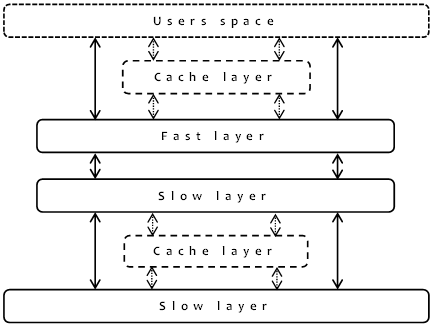
\includegraphics[width=4cm]{kliga1.jpg}
  
  \label{Kliga1}
\end{figure}

\end{center}

Обычно в качестве cache-layer используют RAM-диски созданные в ОЗУ или SSD диски, если необходимо кэширование между  слоями с медленными накопителями. В слой fast-layer, как правило, объединяют быстрые диски, типа SSD, но при этом важно учитывать их технические характеристики. Так, например, при использовании SSD с интерфейсом  NVMe, рекомендуется делать несколько слоев  fast-layer, объединяя в каждый слой SSD накопители одного типа.  В слои slow-layer как правило, объединяют шпиндельные накопители на магнитных дисках (HDD), группируя исходя из их технических характеристик, либо иные типы накопителей, например, ленточные.

Суммарный объем многослойного СХД равен сумме объемов каждого слоя, при этом необходимо учитывать, что по мере заполнения слоя данными, часть его объема может быть зарезервировано для операций миграции данных (до 5\% или более от общей емкости слоя).

Существуют две основные концепции создания многослойных СХД с использованием программных решений.  В рамках первой концепции с помощью программных средств установленных на контроллере СХД для пространства пользователя создается интерфейс доступа к хранилищу данных как устройства блочного типа, таким образом пользователь оперирует с ним как с обычным накопителем. Управление контроллером СХД осуществляется через программный интерфейс, а структура слоев скрыта от пользователя.

В рамках второй концепции возможности создания многослойных СХД реализуется с помощью программного менеджера накопителей в файловой системе (наиболее популярное решения для  хранилища данных модели DAS). Такой подход реализованы, например, в файловых системах как Bcachefs ~\cite{kliga-3}, ZFS ~\cite{kliga-4} и Btrfs ~\cite{kliga-5}. Основным преимуществом этой концепции является то, что пользователь может полностью управлять как слоями так и накопителями в СХД.

Так же важно отметить, что технологии тиринга и кэширования широко  используются в решениях программных систем хранения данных, например, в распределенной файловой системе GlusterFS ~\cite{kliga-7}, или объектном хранилище данных Ceph ~\cite{kliga-6}.

\subsection*{Многоуровневые  системы хранения данных.}

В основу концепции многоуровневых систем хранения данных положен принцип объединения отдельных хранилищ данных в единую СХД с общим центром управления и мониторинга, основанную на модели программно-определяемых  систем хранения данных (software-define storage или SDS). Основным компонентом многоуровневого СХД является контроллер, который осуществляет мониторинг и анализ статистики работы отдельных хранилищ данных, управляем миграцией между уровнями, и обеспечивает подключение новых хранилищ к СХД.  Общая структурная схема многоуровневого СХД приведена ниже.

\begin{center}

\begin{figure}[h!]
  \centering
  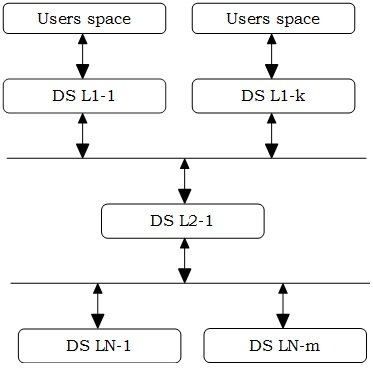
\includegraphics[width=4cm]{kliga2.jpg}
  
  \label{Kliga2}
\end{figure}

\end{center}


\begin{center}\end{center}

На верхнем уровне, как правило, располагают хранилища данных взаимодействующим с пространством пользователя. На втором уровне, как правило, располагают хранилища данных основное назначение которых хранить «холодные данные» с хранилищ первого уровня, и поддерживать миграцию данных между ними. На третьем и ниже уровне могут находится хранилища архивных данных. Основным преимуществом такой модели СХД является оптимизация хранения данных на первом уровне и распределение нагрузки между хранилищами.

Для реализации многоуровневых СХД могут быть использованы различные программные решения, например, в качестве контроллера может быть использован open source проект CorpHD ~\cite{kliga-8}. Одним из его преимуществ является интеграция с объектным хранилищем данных Ceph, и гибкая настройка архитектуры.

Программно-определяемые хранилища данных являются перспективным направлением развития систем хранения данных и поэтому  Linux Foundation в октябре прошлого года объявил о старте нового проекта по созданию Open Controller for Software-Defined Storage ~\cite{kliga-9}, который станет основой для построения открытых решений SDS. Ознакомится с этим новым проектом можно на его официальном ресурсе ~\cite{kliga-10}.

%\subsection*{Ссылки}
\begin{thebibliography}{20}
\bibitem{kliga-1}Flash memory summit \url{https://www.flashmemorysummit.com/}
\bibitem{kliga-2}The official site NVM Express: // \url{http://www.nvmexpress.org/}
\bibitem{kliga-3}Bcachefs: An advanced new filesystem for Linux // \url{http://bcachefs.org/}
\bibitem{kliga-4}ZFS: Zettabyte File System (OpenZFS project) //  \url{http://open-zfs.org/}
\bibitem{kliga-5}Btrfs: Btrfs is a modern CoW filesystem for Linux // \url{https://btrfs.wiki.kernel.org/index.php/Main_Page}
\bibitem{kliga-6}Ceph: The future of storage // \url{https://ceph.com/}
\bibitem{kliga-7}Gluster: Storage for your Cloud // \url{https://www.gluster.org/}
\bibitem{kliga-8}CorpHD: An open source software defined storage controller // \url{https://coprhd.github.io/}
\bibitem{kliga-9}The Linux Foundation creates Open Controller for Software-Defined Storage // \url{https://www.linuxfoundation.org/announcements/linux-foundation-creates-open-controller-for-_software-defined-storage}
\bibitem{kliga-10}OpenSDS Project // \url{https://www.opensds.io/}
\end{thebibliography}

\end{document}

\documentclass[10pt, a5paper]{article}
\usepackage{pdfpages}
\usepackage{parallel}
\usepackage[T2A]{fontenc}
\usepackage{ucs}
\usepackage[utf8x]{inputenc}
\usepackage[polish,english,russian]{babel}
\usepackage{hyperref}
\usepackage{rotating}
\usepackage[inner=2cm,top=1.8cm,outer=2cm,bottom=2.3cm,nohead]{geometry}
\usepackage{listings}
\usepackage{graphicx}
\usepackage{wrapfig}
\usepackage{longtable}
\usepackage{indentfirst}
\usepackage{array}
\newcolumntype{P}[1]{>{\raggedright\arraybackslash}p{#1}}
\frenchspacing
\usepackage{fixltx2e} %text sub- and superscripts
\usepackage{icomma} % коскі ў матэматычным рэжыме
\PreloadUnicodePage{4}

\newcommand{\longpage}{\enlargethispage{\baselineskip}}
\newcommand{\shortpage}{\enlargethispage{-\baselineskip}}

\def\switchlang#1{\expandafter\csname switchlang#1\endcsname}
\def\switchlangbe{
\let\saverefname=\refname%
\def\refname{Літаратура}%
\def\figurename{Іл.}%
}
\def\switchlangen{
\let\saverefname=\refname%
\def\refname{References}%
\def\figurename{Fig.}%
}
\def\switchlangru{
\let\saverefname=\refname%
\let\savefigurename=\figurename%
\def\refname{Литература}%
\def\figurename{Рис.}%
}

\hyphenation{admi-ni-stra-tive}
\hyphenation{ex-pe-ri-ence}
\hyphenation{fle-xi-bi-li-ty}
\hyphenation{Py-thon}
\hyphenation{ma-the-ma-ti-cal}
\hyphenation{re-ported}
\hyphenation{imp-le-menta-tions}
\hyphenation{pro-vides}
\hyphenation{en-gi-neering}
\hyphenation{com-pa-ti-bi-li-ty}
\hyphenation{im-pos-sible}
\hyphenation{desk-top}
\hyphenation{elec-tro-nic}
\hyphenation{com-pa-ny}
\hyphenation{de-ve-lop-ment}
\hyphenation{de-ve-loping}
\hyphenation{de-ve-lop}
\hyphenation{da-ta-ba-se}
\hyphenation{plat-forms}
\hyphenation{or-ga-ni-za-tion}
\hyphenation{pro-gramming}
\hyphenation{in-stru-ments}
\hyphenation{Li-nux}
\hyphenation{sour-ce}
\hyphenation{en-vi-ron-ment}
\hyphenation{Te-le-pathy}
\hyphenation{Li-nux-ov-ka}
\hyphenation{Open-BSD}
\hyphenation{Free-BSD}
\hyphenation{men-ti-on-ed}
\hyphenation{app-li-ca-tion}

\def\progref!#1!{\texttt{#1}}
\renewcommand{\arraystretch}{2} %Іначай формулы ў матрыцы зліпаюцца з лініямі
\usepackage{array}

\def\interview #1 (#2), #3, #4, #5\par{

\section[#1, #3, #4]{#1 -- #3, #4}
\def\qname{LVEE}
\def\aname{#1}
\def\q ##1\par{{\noindent \bf \qname: ##1 }\par}
\def\a{{\noindent \bf \aname: } \def\qname{L}\def\aname{#2}}
}

\def\interview* #1 (#2), #3, #4, #5\par{

\section*{#1\\{\small\rm #3, #4. #5}}

\def\qname{LVEE}
\def\aname{#1}
\def\q ##1\par{{\noindent \bf \qname: ##1 }\par}
\def\a{{\noindent \bf \aname: } \def\qname{L}\def\aname{#2}}
}

\switchlang{be}
\begin{document}
\title{Выкарыстанне вольнага праграмнага забеспячэння ў ЛНУ імя Івана Франка і ЛНМУ імя Данііла Галіцкага \footnote{\url{zlobingg@gmail.com}, \url{http://lvee.org/ru/abstracts/248}}}
\author{С. Апуневич, Г. Злобін, Р. Рикалюк, П. Риковський, \\ Р. Шувар , Ľviv, Ukraine}
\maketitle
\begin{abstract}
The report analyzes 20 years of experience in the implementation of free software at Lviv Ivan I. Franko University and Lviv D. Galitsky University
\end{abstract}

На працягу многіх гадоў львоўская група карыстальнікаў Linux праводзіла агітацыйную працу па ўкараненні вольнага праграмнага забеспячэння ў навучальны працэс навучальных устаноў г. Львова. З 1998 г. пачалося ўкараненне АС Linux у навучальны працэс ЛНМУ імя Данііла Галіцкага. У 2002-2003 гг. было прынята рашэнне дэпутацкай камісіі па пытаннях адукацыі Львоўскага гарадскога савета аб закупцы класаў вучэбнай камп'ютарнай тэхнікі з прадусталяванай АС Linux. Для настаўнікаў школ, якія атрымлівалі камп'ютарную тэхніку з АС Linux, былі праведзены навучальныя курсы па асновах працы ў АС Linux ~\cite{Zlobin-1}. У 2004 г. пачаўся праект па аптымізацыі дыстрыбутыва Debian для карыстання камп'ютарнай тэхнікі з Еўропы, якая падавалася экалагічным арганізацыям Украіны на бязвыплатнай аснове ~\cite{Zlobin-2}. У той жа час пачалося карыстанне АС Linux у навучальным працэсe факультэта электронікі ЛНУ імя Івана Франка. У 2013 г. праз цяжкую сітуацыю з фінансаваннем факультэта з аднаго боку і ў сувязі з пачаткам ціску прадстаўніцтва Microsoft ва Украіне па выкарыстанні ліцэнзійнага ПЗ фірмы Microsoft у навучальных установах Украіны кіраўніцтва факультэта электронікі прыняло рашэнне аб пераводзе навучальных лабараторый на АС Linux.

На жаль, з-за разнамаснай камп'ютарнай тэхнікі ў школах (пачынаючы з ПЭВМ з працэсарам Intel 80486) і супраціў настаўнікаў інфарматыкі адбыўся пераход школ да неліцэнзійнай АС Microsoft Windows і праграмнага забеспячэння для яе. Затое ў ЛНМУ імя Данііла Галіцкага і ЛНУ імя Івана Франка выкарыстоўваецца па сённяшні дзень. Разгледзім сітуацыю па выкарыстанні ВПЗ ў гэтых навучальных установах.

\textbf{І.} Варта падкрэсліць, што пераход навучальнага працэсу ў ЛНМУ імя Данііла Галіцкага на ВПЗ адбыўся пад пагрозай праверкі ліцэнзій ўсталяванага ПЗ -- <<добразычліўцы>> папярэдзілі рэктара ЛНМУ за паўгода да запланаванай праверкі. Сёння ва універсітэце налічваецца больш за 800 камп'ютарных працоўных месцаў,  да некаторых з іх падлучаныя прылады друку, сканеры і шматфункцыянальныя прылады, ёсць 20 камп'ютарных класаў, 10 лекцыйных аўдыторый, якія выкарыстоўваюцца для правядзення ліцэнзійных экзаменаў КРОК і відэаканферэнцый, імітацыйны клас, у якім знаходзяцца 4 праграмуемых манекенаў.

Напрамкі выкарыстання СПО у ЛНМУ:

\begin{itemize}
  \item \textbf{серверныя прымянення} ~--- Linux  (Debian, Ubuntu), Unix (FreeBSD);
  \item \textbf{навучальны працэс} ~--- аперацыйная сістэма \linebreak(Debian,  Ubuntu), офісны пакет (LibreOffice), сродкі праграмавання \linebreak (Bluefish), тэхналогіі тэлемедыцыны, відэаканферэнцсувя-
зі, кантроль за напісаннем ліцэнзійных экзаменаў КРОК, імітацыйны медыцынскі навучальны клас, элементы сістэмы дыстанцыйнага навучання;
  \item \textbf{студэнцкая навуковая праца} ~--- аперацыйная сістэма \linebreak  (Debian, Ubuntu), офісны пакет (LibreOffice), сродкі праграмавання \linebreak (Bluefish), сістэмы кіравання базамі дадзеных (MySQL, Base).
\end{itemize}

Вынікам сказанага з'яўляецца той факт, што:

\begin{enumerate}
  \item У цяперашні час універсітэт цалкам функцыянуе на ліцэнзійным ПЗ, праведзена адпаведная дакументацыйная і арганізацыйная праца.
  \item Шырокі спектр даступнага вольнага праграмнага забеспячэння паказаў магчымасць поўнага забеспячэння працоўнага, навучальнага і навуковага працэсаў у універсітэце.
  \item Пераход на свабоднае праграмнае забеспячэнне дазволіў не толькі пазбегнуць выкарыстання пірацкага праграмнага забеспячэння ў навучальным працэсе, але і паменшыць рызыку нападаў на працоўныя станцыі з боку зламыснікаў і аператараў станцый, паменшылася пагроза віруснай паразы і неабходнасць перманентнай пераўсталёўкі АС.
  \item Працягваецца праца па выкарыстанні элементаў сістэмы дыстанцыйнага навучання.
\end{enumerate}

\textbf{ІІ.} У адрозненне ад ЛНМУ ў ЛНУ імя Івана Франка выкарыстанне ВПЗ не мае ўсёабдымнага характару, а адбываецца ў асобных падраздзяленнях універсітэта. Сёння ў ЛНУ імя Івана Франка налічваецца больш за 2000 камп'ютарных працоўных месцаў, некаторыя з падлучанымі прыладамі друку, сканерамi і шматфункцыянальнымi прыладамi, ёсць 37 камп'ютарных класаў, 20 лекцыйных аўдыторый, якія выкарыстоўваюцца для чытання лекцый з відэапраектарам і правядзення відэаканфэрэнцый. З мэтай забеспячэння ліцэнзійнай АС Microsoft Windows у 2013 была праведзена аплата двухгадовай падпіскі Dream Spark для дзесяці натуральных факультэтаў, аднак два факультэты (фізічны і электронікі і камп'ютарных тэхналогій) гэтай падпіскі не атрымалі з-за грубых памылак у аплікацыйных формах. На гуманітарных факультэтах забяспечанасць ліцэнзійным ПЗ з'яўляецца частковай. На факультэце электронікі і камп'ютарных тэхналогій ВПЗ прысутнiчае ў пяці навучальных лабараторыях, у трох навучальных лабараторыях працуюць дзве аперацыйныя сістэмы: Linux і Microsoft Windows 7 або 10 дзякуючы бясплатнай падпісцы Dream Spark, якую ўдалося аформіць на кафедру радыёфізікі і камп'ютарных тэхналогій пасля правалу платнай падпісцы Dream Spark.

Напрамкі выкарыстання ВПЗ у ЛНУ імя Івана Франка:

\begin{itemize}
  \item \textbf{серверы} ~--- Linux (Debian, Open SuSE,  CentOS), Unix FreeBSD;
  \item \textbf{навучанне} ~--- аперацыйная сістэма (Debian, Open SuSE,\linebreak CentOS, SlackWare), офісныя пакеты (OpenOffice, LibreOffice, Planner), сістэма дыстанцыйнага навучання Moodle, сродкі праграмавання (gcc, IDE Kuzya, IDE CodeBlocks, Qt Creator), матэматычныя пакеты (Octave, SciLab, SMathStudio, Maxima, Labplot), пакеты мадэлявання (Packettracer, Altera Quartus, KiCAD, \linebreak Proteus), кліент-серверныя тэхналогіі;
  \item \textbf{студэнцкая навуковая праца} ~--- аперацыйная сістэма \linebreak (Debian, Open SuSE), офісны пакет (OpenOffice), сродкі праграмавання (gcc, Kuzya IDE, Qt Creator), матэматычныя пакеты (Octave, SciLab, Maxima, Labplot), сістэмы кіравання базамі дадзеных (MySQL), эмулятары апаратных сродкаў і аперацыйных сістэм;
  \item \textbf{навуковыя даследаванні} ~--- аперацыйная сістэма (Debian, Open SuSE), офісны пакет (OpenOffice), сродкі праграмавання (gcc, IDE Kuzya, Qt Creator), матэматычныя пакеты (Octave, SciLab, Maxima, Labplot), арганізацыя вылічальных кластараў і кластараў высокай даступнасці (Scientific Linux, CentOS PaceMaker, Kickstarter, Webmin, SGE, Ganglia, OpenMPI, \linebreak MPICH2, BLAS, FFTW, NorduGrid ARC, Condor, CUDA 5.0 production release).
\end{itemize}

Высновы:

\begin{enumerate}
  \item Нягледзячы на працяглы і няпросты працэс пераходу на ВПЗ у ЛНМУ імя Данііла Галіцкага апынуўся ўдалым ~\cite{Zlobin-3}. Варта адзначыць актыўную падтрымку гэтага працэсу з боку кіраўніцтва ЛНМУ, якая, на думку аўтараў дакладу, мела асабліва матэрыяльны характар. Дзякуючы пераходу на ВПЗ, ЛНМУ імя Данііла Галіцкага не толькі зэканоміў значныя грашовыя сродкі на набыцці ліцэнзій на ПЗ, але і пазбег \linebreak штрафных санкцый за выкарыстанне неліцэнзійнага ПЗ.
  \item Нягледзячы на тое, што ў ЛНУ імя Івана Франка ёсць неабходны кадравы патэнцыял, свабоднае праграмнае забеспячэнне выкарыстоўваецца не ва ўсіх падраздзяленнях універсітэта. Абумоўлена гэта тым, што кіраўніцтва універсітэта не надае належнай увагі ліцэнзійнай чысціні  праграм.
  \item Прыходзіцца канстатаваць, што выкарыстанне прапрыетарнага (і нават неліцэнзійнага) праграмнага забеспячэння прыводзіць да разрыву паміж навучальным працэсам у ЛНУ імя Івана Франка і вытворчым працэсам у ІТ-фірмах Украіны, што дае падставы некаторым аўтарам сцвярджаць пра састарэласць навучальнага працэсу ў навучальных установах Украіны і у прыватнасці ў ЛНУ імя Івана Франко ~\cite{Zlobin-4}.
\end{enumerate}

\begin{thebibliography}{20}

\bibitem{Zlobin-1}Матеріали науково-методичного семінару <<Використання ОС Linux у навчальному процесі середніх і вищих навчальних закладів>>. Львів-2003, 60 с.
\bibitem{Zlobin-2}С. Апуневич, В. Бойко, Г. Злобін, В. Семенюк, С. Кудрик <<Linux — це просто як Borsch>> Львів-2006, 116 с.
\bibitem{Zlobin-3}Курьянович О.В. Використання вільного програмного забезпечення в ЛНМУ імені Данила Галицького. Збірник наукових праць  сьомої науково-практичної конференції FOSS Lviv 2017. -- Львів, Львівський національний університет імені Івана Франка, с. 57
\bibitem{Zlobin-4} \url{http://igate.com.ua/news/13725-top-5-mifov-kotorye-} \url{meshayut-zhit-ukrainskim-programmistam}
\end{thebibliography}
\end{document}

\documentclass[10pt, a5paper]{article}
\usepackage{pdfpages}
\usepackage{parallel}
\usepackage[T2A]{fontenc}
\usepackage{ucs}
\usepackage[utf8x]{inputenc}
\usepackage[polish,english,russian]{babel}
\usepackage{hyperref}
\usepackage{rotating}
\usepackage[inner=2cm,top=1.8cm,outer=2cm,bottom=2.3cm,nohead]{geometry}
\usepackage{listings}
\usepackage{graphicx}
\usepackage{wrapfig}
\usepackage{longtable}
\usepackage{indentfirst}
\usepackage{array}
\newcolumntype{P}[1]{>{\raggedright\arraybackslash}p{#1}}
\frenchspacing
\usepackage{fixltx2e} %text sub- and superscripts
\usepackage{icomma} % коскі ў матэматычным рэжыме
\PreloadUnicodePage{4}

\newcommand{\longpage}{\enlargethispage{\baselineskip}}
\newcommand{\shortpage}{\enlargethispage{-\baselineskip}}

\def\switchlang#1{\expandafter\csname switchlang#1\endcsname}
\def\switchlangbe{
\let\saverefname=\refname%
\def\refname{Літаратура}%
\def\figurename{Іл.}%
}
\def\switchlangen{
\let\saverefname=\refname%
\def\refname{References}%
\def\figurename{Fig.}%
}
\def\switchlangru{
\let\saverefname=\refname%
\let\savefigurename=\figurename%
\def\refname{Литература}%
\def\figurename{Рис.}%
}

\hyphenation{admi-ni-stra-tive}
\hyphenation{ex-pe-ri-ence}
\hyphenation{fle-xi-bi-li-ty}
\hyphenation{Py-thon}
\hyphenation{ma-the-ma-ti-cal}
\hyphenation{re-ported}
\hyphenation{imp-le-menta-tions}
\hyphenation{pro-vides}
\hyphenation{en-gi-neering}
\hyphenation{com-pa-ti-bi-li-ty}
\hyphenation{im-pos-sible}
\hyphenation{desk-top}
\hyphenation{elec-tro-nic}
\hyphenation{com-pa-ny}
\hyphenation{de-ve-lop-ment}
\hyphenation{de-ve-loping}
\hyphenation{de-ve-lop}
\hyphenation{da-ta-ba-se}
\hyphenation{plat-forms}
\hyphenation{or-ga-ni-za-tion}
\hyphenation{pro-gramming}
\hyphenation{in-stru-ments}
\hyphenation{Li-nux}
\hyphenation{sour-ce}
\hyphenation{en-vi-ron-ment}
\hyphenation{Te-le-pathy}
\hyphenation{Li-nux-ov-ka}
\hyphenation{Open-BSD}
\hyphenation{Free-BSD}
\hyphenation{men-ti-on-ed}
\hyphenation{app-li-ca-tion}

\def\progref!#1!{\texttt{#1}}
\renewcommand{\arraystretch}{2} %Іначай формулы ў матрыцы зліпаюцца з лініямі
\usepackage{array}

\def\interview #1 (#2), #3, #4, #5\par{

\section[#1, #3, #4]{#1 -- #3, #4}
\def\qname{LVEE}
\def\aname{#1}
\def\q ##1\par{{\noindent \bf \qname: ##1 }\par}
\def\a{{\noindent \bf \aname: } \def\qname{L}\def\aname{#2}}
}

\def\interview* #1 (#2), #3, #4, #5\par{

\section*{#1\\{\small\rm #3, #4. #5}}

\def\qname{LVEE}
\def\aname{#1}
\def\q ##1\par{{\noindent \bf \qname: ##1 }\par}
\def\a{{\noindent \bf \aname: } \def\qname{L}\def\aname{#2}}
}

\switchlang{en}
\begin{document}
\title{Typical mistakes when submitting a new code to Linux kernel\footnote{\url{andy_shev@mail.ru} \url{http://lvee.org/ru/abstracts/240}}}
\author{Andy Shevchenko, Espoo, Finland}
\maketitle
\begin{abstract}
Code review is a crucial part of developing a stable and robust open source project, such as Linux kernel. New comers and surprisingly many active and known contributors have been doing same mistakes, like using non-scalable APIs, over and over. How can we eliminate or avoid them? Looking at the patterns the best practices would be suggested. In addition, relatively new Linux kernel APIs, such as Unified Device Properties, will be discussed.
\end{abstract}
\subsubsection*{Introduction}

According to the Linux kernel v4.11 development statistics ~\cite{Shevchenko1} the code base is grown by nearly 300,000 lines. It means that from now on many of new drivers and other modules are in the vanilla kernel. While performing review on some of the drivers I have noticed that even oldbies have been making same mistakes over and over when submitting a new code. Majority of the issues is poor knowledge of the library APIs in the kernel. For drivers it includes, for example, Device Resource Management API ~\cite{Shevchenko2}, ~\cite{Shevchenko3} or Unified Device Properties API ~\cite{Shevchenko4}, while other modules re-implement simple helper functions, like hex2bin(), from the internal library. Besides that driver developers often are focusing on single CPU architecture or hardware platform which makes the code not so scalable. In the following chapters the most occurred mistakes will be considered. In some cases the non-obvious issues would be discussed, e.g. devm\_request\_threaded\_irq() coexistence together with tasklets and 64-bit hardware registers access and handling.

\subsubsection*{Device Resource Management}

Device Resource Management API ~\cite{Shevchenko2} ~\cite{Shevchenko3} is quite old idea (it dates back to 2007!), that is still evolving, though developers don’t use or use it in a suboptimal way.

The most recent example I have met in ~\cite{Shevchenko5} is the following piece of code:

\lstset{ %
language=C,                 % выбор языка для подсветки (здесь это С)
basicstyle=\small\sffamily, % размер и начертание шрифта для подсветки кода
breaklines=true,           % автоматически переносить строки (да\нет)
breakatwhitespace=false, % переносить строки только если есть пробел
}
\begin{lstlisting}
    ret = of_address_to_resource(np, 0, &res_xbar);
    if (ret) {
        dev_err(dev, "Failed to get xbar resources");
        return ret;
    }
    if (!devm_request_mem_region(dev, res_xbar.start, resource_size(&res_xbar), res_xbar.name)) {
        dev_err(dev, "Failed to get xbar resources");
        return -ENODEV;
    }
    xbar_membase = devm_ioremap_nocache(dev, res_xbar.start, resource_size(&res_xbar));
    if (!xbar_membase) {
        dev_err(dev, "Failed to remap xbar resources");
        return -ENODEV;
    }
\end{lstlisting}

Obviously the developer is not familiar with non-device tree platforms and Device Resource Management API. The better approach is just missed, i.e.

\lstset{ %
language=C,                 % выбор языка для подсветки (здесь это С)
basicstyle=\small\sffamily, % размер и начертание шрифта для подсветки кода
breaklines=true,           % автоматически переносить строки (да\нет)
breakatwhitespace=false, % переносить строки только если есть пробел
}
\begin{lstlisting}
    res_xbar = platform_get_resource(pdev, IORESOURCE_MEM, 0);
    xbar_membase = devm_ioremap_resource(dev, res_xbar);
    if (IS_ERR(xbar_membase))
        return PTR_ERR(xbar_membase);
\end{lstlisting}

In the end we got much simpler code, resource provider agnostic — it will work on Device Tree, ACPI, or legacy platform data enabled platforms.

Of course there are some nuances when the driver is converted to new API. One of them is a good understanding when it’s safe to use devm\_request\_threaded\_irq(). For example, if driver is using tasklets the IRQ handler should be removed before tasklets. It will guarantee that no more tasks are scheduled on non-existing data.

Nevertheless previously mentioned examples maybe are not the best ones when we speak about hardware IP blocks which would have been using on various CPU architectures and platforms, where Unified Device property API is a big helper.

\subsubsection*{Unified Device Properties}

Back to 2014 Rafael Wysocki had submitted a new common API ~\cite{Shevchenko4} for drivers to get device properties in resource provider agnostic way. It means legacy platform data, ACPI, or Device Tree resource providers do not require special handling anymore in the drivers.

Besides that few other subsystems, i.e. GPIO, I2C, SPI, were updated accordingly to hide resource provider details in their core parts.

One of the recent and nice example of conversion to new API is the commit 95129b6f0806 (''NFC: pn544: Get rid of code duplication in probe()'') ~/cite{Shevchenko6} along with few preparations in vanilla kernel.

While the above is related mostly to the drivers, the small parts of the rest of the code might have been reinventing the wheel, such as hex2bin() helper or even more often helpers to dump small buffers in hexadecimal or escaped format.

\subsubsection*{Special extensions of \%p}

How often do you need to dump several bytes from the buffer in the log to reveal some details about an error? I’m pretty sure it have been happening sometimes. Linux kernel vsnprintf() and thus its derivatives implements special extensions of \%p specifier ~\cite{Shevchenko7}. In particular, instead of reinventing hexdump functionality the developer may just use something like:

\lstset{ %
language=C,                 % выбор языка для подсветки (здесь это С)
basicstyle=\small\sffamily, % размер и начертание шрифта для подсветки кода
breaklines=true,           % автоматически переносить строки (да\нет)
breakatwhitespace=false, % переносить строки только если есть пробел
}
\begin{lstlisting}
    u8 data[100};
    ...
    pr_debug("Buf: %*phC\n", (int)sizeof(data), data); /* only first 64 bytes! */
\end{lstlisting}

That code will dump first 64 bytes in hexadecimal format with ‘:’ (colon) as a delimiter.

There are also many other extensions, e.g. printing buffer in escaped format, IPv4 and IPv6 addresses, MAC addresses, architecture dependent types, device resources and so on.

\subsubsection*{Recommendations on how prepare changes to Linux kernel}

When developer consider the code tested and ready for submission the last things to be worth doing are:

\begin{itemize}
  \item \textbf{Check the code again for duplication.}
  \item \textbf{Take the material from the above chapters into consideration when doing drivers.}
  \item \textbf{Establish internal mailing list for review and review process if it’s not done yet.}
  \item \textbf{If in doubt, feel free to ask.}
\end{itemize}

%\subsubsection*{References}
\begin{thebibliography}{99}

\bibitem{Shevchenko1}: 4.11 Kernel development statistics \url{https://lwn.net/Articles/720336/}
\bibitem{Shevchenko2}: Devres -- Managed Device Resource \url{https://www.kernel.org/doc/Documentation/driver-model/devres.txt}
\bibitem{Shevchenko3}: The managed resource API \url{https://lwn.net/Articles/222860/}
\bibitem{Shevchenko4}: Unified Device Properties Interface for ACPI and Device Trees \url{http://events.linuxfoundation.org/sites/events/files/slides/unified_properties_API_0.pdf}
\bibitem{Shevchenko5}: MIPS: lantiq: Convert the xbar driver to a platform\_driver \url{https://patchwork.ozlabs.org/patch/765088/}
\bibitem{Shevchenko6}: NFC: pn544: Get rid of code duplication in probe \url{https://git.kernel.org/pub/scm/linux/kernel /git/torvalds/linux.git/commit/?id=95129b6f0806d1ba6109dc1df4d9753ad3d4a94c}
\bibitem{Shevchenko7}: printk() formats \url{https://www.kernel.org/doc/Documentation/printk-formats.txt}
\end{thebibliography}
\end{document}

\documentclass[10pt, a5paper]{article}
\usepackage{pdfpages}
\usepackage{parallel}
\usepackage[T2A]{fontenc}
\usepackage{ucs}
\usepackage[utf8x]{inputenc}
\usepackage[polish,english,russian]{babel}
\usepackage{hyperref}
\usepackage{rotating}
\usepackage[inner=2cm,top=1.8cm,outer=2cm,bottom=2.3cm,nohead]{geometry}
\usepackage{listings}
\usepackage{graphicx}
\usepackage{wrapfig}
\usepackage{longtable}
\usepackage{indentfirst}
\usepackage{array}
\newcolumntype{P}[1]{>{\raggedright\arraybackslash}p{#1}}
\frenchspacing
\usepackage{fixltx2e} %text sub- and superscripts
\usepackage{icomma} % коскі ў матэматычным рэжыме
\PreloadUnicodePage{4}

\newcommand{\longpage}{\enlargethispage{\baselineskip}}
\newcommand{\shortpage}{\enlargethispage{-\baselineskip}}

\def\switchlang#1{\expandafter\csname switchlang#1\endcsname}
\def\switchlangbe{
\let\saverefname=\refname%
\def\refname{Літаратура}%
\def\figurename{Іл.}%
}
\def\switchlangen{
\let\saverefname=\refname%
\def\refname{References}%
\def\figurename{Fig.}%
}
\def\switchlangru{
\let\saverefname=\refname%
\let\savefigurename=\figurename%
\def\refname{Литература}%
\def\figurename{Рис.}%
}

\hyphenation{admi-ni-stra-tive}
\hyphenation{ex-pe-ri-ence}
\hyphenation{fle-xi-bi-li-ty}
\hyphenation{Py-thon}
\hyphenation{ma-the-ma-ti-cal}
\hyphenation{re-ported}
\hyphenation{imp-le-menta-tions}
\hyphenation{pro-vides}
\hyphenation{en-gi-neering}
\hyphenation{com-pa-ti-bi-li-ty}
\hyphenation{im-pos-sible}
\hyphenation{desk-top}
\hyphenation{elec-tro-nic}
\hyphenation{com-pa-ny}
\hyphenation{de-ve-lop-ment}
\hyphenation{de-ve-loping}
\hyphenation{de-ve-lop}
\hyphenation{da-ta-ba-se}
\hyphenation{plat-forms}
\hyphenation{or-ga-ni-za-tion}
\hyphenation{pro-gramming}
\hyphenation{in-stru-ments}
\hyphenation{Li-nux}
\hyphenation{sour-ce}
\hyphenation{en-vi-ron-ment}
\hyphenation{Te-le-pathy}
\hyphenation{Li-nux-ov-ka}
\hyphenation{Open-BSD}
\hyphenation{Free-BSD}
\hyphenation{men-ti-on-ed}
\hyphenation{app-li-ca-tion}

\def\progref!#1!{\texttt{#1}}
\renewcommand{\arraystretch}{2} %Іначай формулы ў матрыцы зліпаюцца з лініямі
\usepackage{array}

\def\interview #1 (#2), #3, #4, #5\par{

\section[#1, #3, #4]{#1 -- #3, #4}
\def\qname{LVEE}
\def\aname{#1}
\def\q ##1\par{{\noindent \bf \qname: ##1 }\par}
\def\a{{\noindent \bf \aname: } \def\qname{L}\def\aname{#2}}
}

\def\interview* #1 (#2), #3, #4, #5\par{

\section*{#1\\{\small\rm #3, #4. #5}}

\def\qname{LVEE}
\def\aname{#1}
\def\q ##1\par{{\noindent \bf \qname: ##1 }\par}
\def\a{{\noindent \bf \aname: } \def\qname{L}\def\aname{#2}}
}

\begin{document}
\title{Make your own USB gadget\footnote{\url{andrzejtp2010@gmail.com} \url{http://lvee.org/ru/abstracts/241}}}
\author{Andrzej Pietrasiewicz, Warsaw, Poland}
\maketitle
\begin{abstract}
A widely accepted standard for adding functionality to computer systems is the USB bus. GNU/Linux systems have long been supporting USB hosts, but a less known fact is that they also support USB devices. The traditional way of preparing support for devices includes creating a kernel module, which makes the process significantly more difficult. A new approach is presented, which requires only shell scripting.
\end{abstract}
\subsection*{Introduction}

Serial communication has been present since very early days of electronic computers in the semiconductor era. In serial communication in principle the data stream is finally decomposed into individual bits which are transmitted over the medium and such a process can be implemented in various ways. The most widely employed standard used to be RS-232-C, which was formalized in 1969 ~\cite{Pietrasiewicz1}. Since then it has found widespread acceptance and served its purposes very well for the next 20  years. However, with processing speed increasing rapidly a demand for faster transmission appeared. On the other hand computer systems miniaturization progressing stimulated dropping the usage of voltages higher than 5V. These, among others, have been the reasons to introduce a newer standard, better suited for the then current and future needs. Such a standard was USB, the Universal Serial Bus ~\cite{Pietrasiewicz2}, first specified in 1996. The standard was and still is successful, and there have been a number of major updates to it in 1998 ~\cite{Pietrasiewicz3}, 2000 ~\cite{Pietrasiewicz4}, 2008 ~\cite{Pietrasiewicz5} and 2013 ~\cite{Pietrasiewicz6}.

\subsection*{USB high level architecture}

USB is a bus with one host node and many (up to 127) device nodes physically connected in a „tree” topology. According to the standard the logical topology is in fact a „star” topology with the host being the central unit. The roles in the communication are strictly defined. In particular, a dedicated piece of hardware is needed at both sides of the cable (host-device) to maintain the physical aspects of data transmission over the medium and to maintain logical interaction \linebreak between the communicating parties. While the host part is in \linebreak widespread use in all modern PCs (and other equipment) and is \linebreak supported by GNU/Linux, the devices tend to be specialized appliances or gadgets like printers, pendrives, broadband modems or digital TV receivers.

\subsection*{USB gadget support in GNU/Linux}

GNU/Linux systems have in-kernel support for the device part of USB communication, which means that provided the system running GNU/Linux is equipped with appropriate hardware it can be turned into a full USB device controlled by Linux kernel and userspace running on it ~\cite{Pietrasiewicz7}. Device (also called gadget) supporting code is organized in a so-called composite framework ~\cite{Pietrasiewicz8}, which factors out code common to all USB functions implemented on the one hand, and delegates function-specific implementation to separate „function” files. USB standard \linebreak requires that a device provides at least one configuration, and in a configuration there are a number of interfaces providing interesting services to the USB host. There can be more than one configuration, but only one can be active at a time. Composite devices are possible, where there are a number of functions (interfaces) and configurations available, e.g. a mass storage device composed with a broadband modem, where the mass storage device contains driver software for the modem. While Linux kernel provides a rather wide choice of USB functions (interfaces), they need to be somehow combined into a device. The traditional way of composing such USB devices has been to provide dedicated kernel modules, where the choice of USB functions, their composition into configurations and the gadget identity is hardcoded. Such an approach makes it difficult to compose new devices as it requires the skills needed to program Linux kernel. And even provided this difficulty is overcome, the code of the new module must be maintained either in-house or accepted by the community to become a part of officially maintained Linux kernel. Either of the two is not necessarily an easy task.

\subsection*{New interface for USB gadget composition}

Around the beginning of 2015 a process of adding support for \linebreak composing USB gadgets at runtime out of existing USB functions has been completed. The new approach still uses the composite framework, but the added functionality allows the components to be specified and composed into a gadget at runtime, which means that it is the user (the system administrator) who controls the gadget creation process. The interface used for this purpose is based on ConfigFS, which in turn is a pseudo file system similar to sysfs, so all interactions of the user controlling gadget creation use well known file system concepts. These are: directory creation/removal (creating gadget's configuration), symbolic link creation/removal (grouping things together, e.g. assigning functions to configurations), file writing/reading (specifying gadget \linebreak parameters, querying gadget parameters).

The new interface for runtime composing USB gadgets out of existing functions allows new interesting possibilities. Among them is the helper userspace library, libusbgx ~\cite{Pietrasiewicz9}. It encapsulates the „bare” ConfigFS interface in an easy-to-use C interface. It also supports so called gadget schemes, which allow specifying gadget's composition and identity in a declarative style configuration file, rather than using an imperative style shell scripting. The former allows the gadget creator to concentrate on what the gadget is going to be composed of, while the latter forces the creator to also know how the ConfigFS interface works. Such declarative gadget schemes enable future use of the framework e.g. for distributing gadget schemes as installable applications.

\begin{thebibliography}{99}

\bibitem{Pietrasiewicz1} EIA standard RS-232-C: Interface between Data Terminal Equipment and Data Communication Equipment Employing Serial Binary Data Interchange. Washington, USA: Electronic Industries Association, Engineering Department. 1969. OCLC 38637094 / ITU-T V.24

\bibitem{Pietrasiewicz2} Universal Serial Bus Specification, 1996 \url{http://fl.hw.cz/docs/usb/usb10doc.pdf}

\bibitem{Pietrasiewicz3} Universal Serial Bus Specification, 1998 \url{ http://esd.cs.ucr.edu/webres/usb11.pdf}

\bibitem{Pietrasiewicz4} Universal Serial Bus Specification, 2000,\url{ http://www.usb.org/developers/docs/usb20\_docs/usb\_20\_033017.zip}

\bibitem{Pietrasiewicz5} Universal Serial Bus Specification, 2008,\url{ http://www.usb.org/developers/docs/documents\_archive/usb\_30\_spec\_070113.zip}

\bibitem{Pietrasiewicz6} Universal Serial Bus Specification, 2013,\url{ http://www.usb.org/developers/docs/usb\_31\_080416.zip}

\bibitem{Pietrasiewicz7} Andrzej Pietrasiewicz, „Make your own usb gadget”, LinuxCon North America 2014, Chicago, USA,\url{ http://events.linuxfoundation.org/sites/events/files/slides/LinuxConNA-Make-your-own-USB-gadget-Andrzej.Pietrasiewicz.pdf}
\bibitem{Pietrasiewicz8} Michał Nazarewicz, „The USB composite framework”, 
\url{https://lwn.net/Articles/395712/, 2010}

\bibitem{Pietrasiewicz9} \url{https://github.com/libusbgx/libusbgx}
\end{thebibliography}
\end{document}

\documentclass[10pt, a5paper]{article}
\usepackage{pdfpages}
\usepackage{parallel}
\usepackage[T2A]{fontenc}
\usepackage{ucs}
\usepackage[utf8x]{inputenc}
\usepackage[polish,english,russian]{babel}
\usepackage{hyperref}
\usepackage{rotating}
\usepackage[inner=2cm,top=1.8cm,outer=2cm,bottom=2.3cm,nohead]{geometry}
\usepackage{listings}
\usepackage{graphicx}
\usepackage{wrapfig}
\usepackage{longtable}
\usepackage{indentfirst}
\usepackage{array}
\newcolumntype{P}[1]{>{\raggedright\arraybackslash}p{#1}}
\frenchspacing
\usepackage{fixltx2e} %text sub- and superscripts
\usepackage{icomma} % коскі ў матэматычным рэжыме
\PreloadUnicodePage{4}

\newcommand{\longpage}{\enlargethispage{\baselineskip}}
\newcommand{\shortpage}{\enlargethispage{-\baselineskip}}

\def\switchlang#1{\expandafter\csname switchlang#1\endcsname}
\def\switchlangbe{
\let\saverefname=\refname%
\def\refname{Літаратура}%
\def\figurename{Іл.}%
}
\def\switchlangen{
\let\saverefname=\refname%
\def\refname{References}%
\def\figurename{Fig.}%
}
\def\switchlangru{
\let\saverefname=\refname%
\let\savefigurename=\figurename%
\def\refname{Литература}%
\def\figurename{Рис.}%
}

\hyphenation{admi-ni-stra-tive}
\hyphenation{ex-pe-ri-ence}
\hyphenation{fle-xi-bi-li-ty}
\hyphenation{Py-thon}
\hyphenation{ma-the-ma-ti-cal}
\hyphenation{re-ported}
\hyphenation{imp-le-menta-tions}
\hyphenation{pro-vides}
\hyphenation{en-gi-neering}
\hyphenation{com-pa-ti-bi-li-ty}
\hyphenation{im-pos-sible}
\hyphenation{desk-top}
\hyphenation{elec-tro-nic}
\hyphenation{com-pa-ny}
\hyphenation{de-ve-lop-ment}
\hyphenation{de-ve-loping}
\hyphenation{de-ve-lop}
\hyphenation{da-ta-ba-se}
\hyphenation{plat-forms}
\hyphenation{or-ga-ni-za-tion}
\hyphenation{pro-gramming}
\hyphenation{in-stru-ments}
\hyphenation{Li-nux}
\hyphenation{sour-ce}
\hyphenation{en-vi-ron-ment}
\hyphenation{Te-le-pathy}
\hyphenation{Li-nux-ov-ka}
\hyphenation{Open-BSD}
\hyphenation{Free-BSD}
\hyphenation{men-ti-on-ed}
\hyphenation{app-li-ca-tion}

\def\progref!#1!{\texttt{#1}}
\renewcommand{\arraystretch}{2} %Іначай формулы ў матрыцы зліпаюцца з лініямі
\usepackage{array}

\def\interview #1 (#2), #3, #4, #5\par{

\section[#1, #3, #4]{#1 -- #3, #4}
\def\qname{LVEE}
\def\aname{#1}
\def\q ##1\par{{\noindent \bf \qname: ##1 }\par}
\def\a{{\noindent \bf \aname: } \def\qname{L}\def\aname{#2}}
}

\def\interview* #1 (#2), #3, #4, #5\par{

\section*{#1\\{\small\rm #3, #4. #5}}

\def\qname{LVEE}
\def\aname{#1}
\def\q ##1\par{{\noindent \bf \qname: ##1 }\par}
\def\a{{\noindent \bf \aname: } \def\qname{L}\def\aname{#2}}
}

\switchlang{ru}
\begin{document}
\title{О Модели Данных SQL/JSON}
\author{Андреев Юрий, Санкт-Петербург, РФ\footnote{\url{andreev.yurij@gmail.com} \url{http://lvee.org/ru/abstracts/247}}}
\maketitle
\begin{abstract}
An SQL/JSON model is a part of SQL 2016 Standard\cite{AY1} which describes a JSON data model for SQL.
It describes a \textit{jsonpath} data type as a path language and nine functions to deal with JSON data.
A new type of queries will be shown on a special branch of PostgreSQL.
\end{abstract}

\subsection*{Предисловие}
В новою редакцию стандарта SQL\cite{AY1} была включена SQL/JSON модель.
Это означает, что стандарт теперь предполагает работу со слабо-структурированными
данными в JSON формате\cite{AY2}. СУБД Postgres имеет долгую историю поддержки такого типа данных
и теперь идет работа по поддержке новых возможностей стандарта.
Далее мы покажем, какие преимущества дает способ хранения в JSON формате и как 
предполагается делать запросы к таким данным.

\subsection*{Слабо-структурированные данные}
Однажды Землю Винни-Пуха посетил Слон
\footnote{Слон --- это символ PostgreSQL}.
Он вышел на прогулку в прошлую среду
\footnote{на самом деле, еще не вышел. Далее используется разрабатываемая sqljson ветка PostgreSQL.}
и еще не бывал в этих местах.
Ему стало очень интересно узнать, кто здесь живет.
Сначала он навестил Кролика,
\begin{verbatim}
INSERT INTO elephant (name) VALUES ('Кроличья нора'); 
\end{verbatim}
Слон запоминает все в таблицу 
\texttt{elephant}\footnote{названия таблиц и колонок можно также писать и по-русски},
где каждая запись состоит из двух полей: 
имени в обычном строковом представлении (\texttt{name})
и деталей в формате JSON (\texttt{details})
\footnote{на текущий момент, запросы нового типа работают с  данными только в формате JSONB (более строгой форме JSON)}.
Слон узнал \texttt{details}: 
\begin{verbatim}
{
    "жители":"Кролик",
    "проход":"очень узкий",
    "мёд":"ещё немного"
}
\end{verbatim}
Потом он обошел вокруг Дуба (\texttt{name = "Высокий-превысокий Дуб"}), \texttt{details}:
\begin{verbatim}
{
    "жители":"Пчёлы",
    "высота":"так высоко",
    "мёд":"неправильный"
}
\end{verbatim}
Наконец, Cлон зашел к Пяточку (\texttt{name = "Домик Пяточка"}):
\begin{verbatim}
{
    "жители":"Пяточёк",
    "шарики":["синий", "зелёный"]
}
\end{verbatim}
Пяточек сказал, что у него есть друг, с которым Слон обязательно должен познакомиться.
Настала медовая пора и было жарко.
Переходя по мосту реку, он опустил хобот и немного расширился от выпитой воды. 
Слоны вообще хорошо расширяются.
Теперь Слон был готов ко встрече с Винни-Пухом.

\subsection*{Модель SQL/JSON}
Но как же Винни-Пух будет общаться со Слоном?
Всем известно, что слоны разговаривают на SQL. 
Наш же успел понабраться новомодных словечек, и начинает использовать SQL/JSON.
Для запросов в стандарте описаны новые функции, с префиксом \texttt{JSON\_},
а также язык \textit{jsonpath} для навигации по JSON 
(частичный аналог XPath для XML; см. также описание в \cite{AY3}),
выражения на котором передается во втором аргументе. 
Поможем Винни-Пуху. Ему интересны медовые места, для этого он должен спросить Слона:
\begin{verbatim}
SELECT name 
FROM elephant 
WHERE JSON_EXISTS(details,'$.мёд')
------------------------
 Кроличья нора
 Высокий-превысокий Дуб
\end{verbatim}
А насколько Дуб высокий?
\begin{verbatim}
SELECT JSON_VALUE(details, '$.высота') 
FROM elephant 
WHERE name='Высокий-превысокий Дуб';
--------------
 "так высоко"
\end{verbatim}
Чтобы на него подняться, нужны шарики. 
Они есть у Пяточка, это также легко узнать. А сколько же их? 
\begin{verbatim}
SELECT JSON_QUERY(details, '$.шарики.size()') 
FROM elephant 
WHERE name = 'Домик Пяточка';
----------
 2
\end{verbatim}
Есть ли синий? t(True)/f(False)
\begin{verbatim}
SELECT 
    JSON_EXISTS(details, '$.шарики[*] ? (@ == "синий")') 
FROM elephant WHERE name = 'Домик Пяточка';
----------
 t
\end{verbatim}

Пока Винни-Пух летает за медом, можно заметить, что
преимущество JSON/SQL модели, помимо прочего, заключается в том, что Винни-Пух
может придумать множество других запросов, 
а Слон, гуляя, может произвольно дополнять свои знания:
выделить улей, как отдельный объект в составе Дуба; 
добавить содержание надписей на вывесках у домиков, если таковые имеются.
При этом данные будут храниться компактно, и не надо будет перестраивать основную таблицу, что бывает затратно.

Тем  временем у Винни-Пуха появились новые запросы, он собирается в гости к Кролику, чтобы немного подкрепиться.  
Что об этом подумает сам Кролик, мы не узнаем, а вот о чем и как думает Слон мы можем всегда поинтересоваться,
так как Слон --- это open source.

\begin{thebibliography}{9}
\bibitem{AY1} Стандарт SQL, ISO/IEC 9075-2:2016, \url{https://www.iso.org/standard/63556.html}
\bibitem{AY2} JSON формат, RFC 7159, \url{https://www.rfc-editor.org/info/rfc7159}, 
\bibitem{AY3} jsonpath, \url{http://goessner.net/articles/JsonPath/}
\end{thebibliography}

\end{document}

\documentclass[10pt, a5paper]{article}
\usepackage{pdfpages}
\usepackage{parallel}
\usepackage[T2A]{fontenc}
\usepackage{ucs}
\usepackage[utf8x]{inputenc}
\usepackage[polish,english,russian]{babel}
\usepackage{hyperref}
\usepackage{rotating}
\usepackage[inner=2cm,top=1.8cm,outer=2cm,bottom=2.3cm,nohead]{geometry}
\usepackage{listings}
\usepackage{graphicx}
\usepackage{wrapfig}
\usepackage{longtable}
\usepackage{indentfirst}
\usepackage{array}
\newcolumntype{P}[1]{>{\raggedright\arraybackslash}p{#1}}
\frenchspacing
\usepackage{fixltx2e} %text sub- and superscripts
\usepackage{icomma} % коскі ў матэматычным рэжыме
\PreloadUnicodePage{4}

\newcommand{\longpage}{\enlargethispage{\baselineskip}}
\newcommand{\shortpage}{\enlargethispage{-\baselineskip}}

\def\switchlang#1{\expandafter\csname switchlang#1\endcsname}
\def\switchlangbe{
\let\saverefname=\refname%
\def\refname{Літаратура}%
\def\figurename{Іл.}%
}
\def\switchlangen{
\let\saverefname=\refname%
\def\refname{References}%
\def\figurename{Fig.}%
}
\def\switchlangru{
\let\saverefname=\refname%
\let\savefigurename=\figurename%
\def\refname{Литература}%
\def\figurename{Рис.}%
}

\hyphenation{admi-ni-stra-tive}
\hyphenation{ex-pe-ri-ence}
\hyphenation{fle-xi-bi-li-ty}
\hyphenation{Py-thon}
\hyphenation{ma-the-ma-ti-cal}
\hyphenation{re-ported}
\hyphenation{imp-le-menta-tions}
\hyphenation{pro-vides}
\hyphenation{en-gi-neering}
\hyphenation{com-pa-ti-bi-li-ty}
\hyphenation{im-pos-sible}
\hyphenation{desk-top}
\hyphenation{elec-tro-nic}
\hyphenation{com-pa-ny}
\hyphenation{de-ve-lop-ment}
\hyphenation{de-ve-loping}
\hyphenation{de-ve-lop}
\hyphenation{da-ta-ba-se}
\hyphenation{plat-forms}
\hyphenation{or-ga-ni-za-tion}
\hyphenation{pro-gramming}
\hyphenation{in-stru-ments}
\hyphenation{Li-nux}
\hyphenation{sour-ce}
\hyphenation{en-vi-ron-ment}
\hyphenation{Te-le-pathy}
\hyphenation{Li-nux-ov-ka}
\hyphenation{Open-BSD}
\hyphenation{Free-BSD}
\hyphenation{men-ti-on-ed}
\hyphenation{app-li-ca-tion}

\def\progref!#1!{\texttt{#1}}
\renewcommand{\arraystretch}{2} %Іначай формулы ў матрыцы зліпаюцца з лініямі
\usepackage{array}

\def\interview #1 (#2), #3, #4, #5\par{

\section[#1, #3, #4]{#1 -- #3, #4}
\def\qname{LVEE}
\def\aname{#1}
\def\q ##1\par{{\noindent \bf \qname: ##1 }\par}
\def\a{{\noindent \bf \aname: } \def\qname{L}\def\aname{#2}}
}

\def\interview* #1 (#2), #3, #4, #5\par{

\section*{#1\\{\small\rm #3, #4. #5}}

\def\qname{LVEE}
\def\aname{#1}
\def\q ##1\par{{\noindent \bf \qname: ##1 }\par}
\def\a{{\noindent \bf \aname: } \def\qname{L}\def\aname{#2}}
}

\begin{document}
\title{Электромиографическое распознавание движений пальцев руки человека на базе Arduino\footnote{\url{shadimx@gmail.com} \url{http://lvee.org/ru/abstracts/245}}}
\author{Вадим Шамонин, Брест, Belarus}
\maketitle
\begin{abstract}
An open hardware project for the electromyography measurements is presented. Arduino platform is engaged in getting data from the epidermic sensors and passing them to the receiving software to detect and classify muscle activity. Results of fingers movements recognition are presented for two sensors placement approaches.
\end{abstract}
\subsection*{Введение}

В настоящее время разрабатывается большое количество устройств, позволяющих использовать пальцы рук в качестве источника управляющих сигналов. Все их можно разделить на три категории:

\begin{itemize}
  \item механические манипуляторы, повторяющие движения человеческой руки;
  \item взаимодействие с объектами в системах виртуальной и/или дополненной реальности;
  \item мониторинг биологических параметров организма.
\end{itemize}

Применения электромиографического метода (ЭМГ) для этого круга задач делает возможным не только распознавание степени сгибания пальцев с высокой точностью, но также позволяет использовать полученные данные для выявления медицинских отклонений пациента. ЭМГ также предоставляет новые возможности в области реабилитации после инсульта. К примеру, антропоморфная робототехника, применяемая в медицине, позволяет регулярно разгибать руку у человека, который в результате болезни потерял такую возможность (это называется нейрореабилитацией, и применяется в том числе после инсультов и нейротравм).

\begin{center}

\begin{figure}[h!]
  \centering
  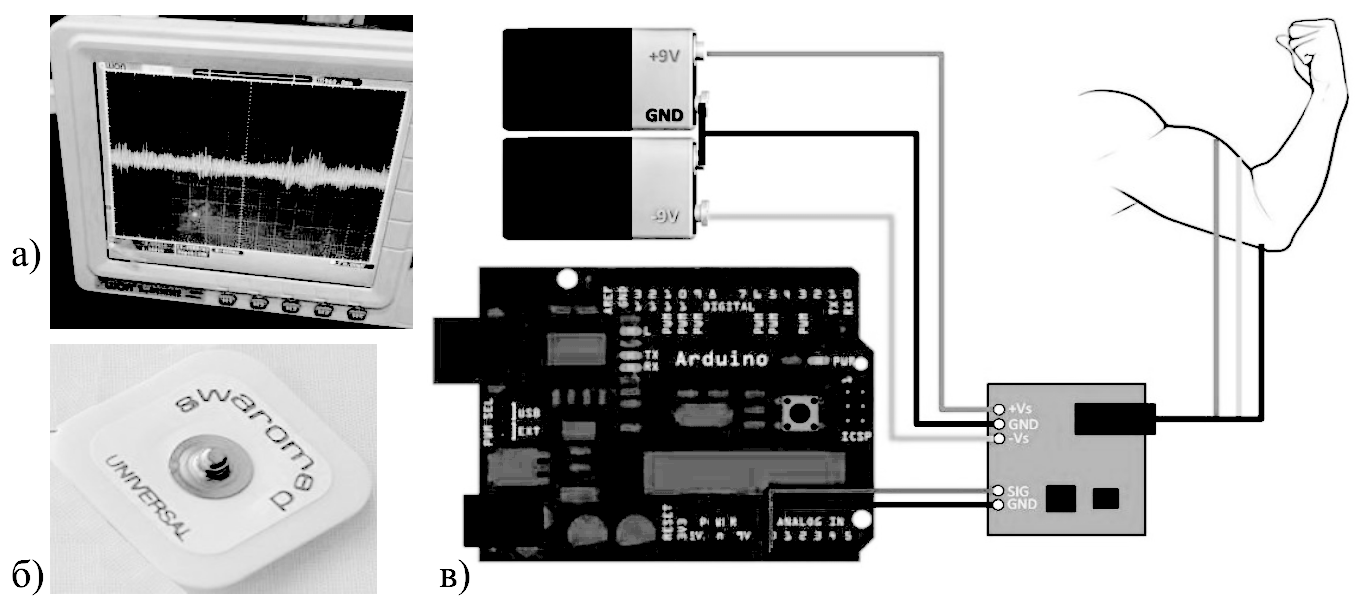
\includegraphics[width=9cm]{Shamonin1.PNG}
  \caption{Используемые накожные электроды Ag/AgCl (а), визуализация сигналов с них, снятых без усиления (б) и схема подключения усилителя (в)}
  \label{Shamonin1}

\end{figure}

\end{center}


\subsection*{Аппаратная платформа и особенности реализации}

Разработанное устройство построено на основе платформы Arduino. Проект разрабатывается как open hardware, наработки доступны по адресу \url{https://github.com/shadimx}.

При помощи неё данные обрабатываются при подключении к ПК. Электрическую активность мышц при помощи накожных Ag-электродов, широко используемых в медицинских целях при записи ЭКГ (рис. ~\ref{Shamonin1}). Для более точного выявления биопотенциалов используется специализированный OpenHardware-модуль цифрового усиления сигналов для Arduino — muscle sencor v3 от sparkfun (рис. ~\ref{Shamonin1}).

\subsection*{Особенности измерений}

Для решения задачи распознавания движений пальцами важную роль играет методика регистрации ЭМГ. В работе рассмотрены 2 методики регистрации сигналов при использовании неинвазивной ЭМГ.

В рамках 1-й методики положения №4 и №5, также как и №6 и №7 (рис. ~\ref{Shamonin2}) регистрировались одним электродом. Сигналы записывались относительно канала “Reference”, положение которого выбиралось на участке выше локтя, на котором отсутствуют сокращения мышц при движении пальцами. Электрод канала “Ground” располагался в районе плечевого сустава. В рамках 2-й методики те же положения регистрировались отдельными электродами, при положении электродов каналов “Reference” и “Ground” таком же, как в 1-й методике. Кроме того, снималось также 5 дифференциальных каналов между положениями 1 и 2; 3 и 4; 5 и 6; 7 и 8; 9 и 10. В результате методика с использованием дифференциальных каналов позволила улучшить отношение сингал/шум, что обеспечило существенно лучшее качество распознавания движений классификатором (рис. ~\ref{Shamonin2}). Отметим, что использование некоторых каналов не улучшает работу классификатора. Для 2-й методики достаточно использовать 5 дифференциальных и 2 отдельных канала.

\begin{center}
\begin{figure}[h!]
  \centering
  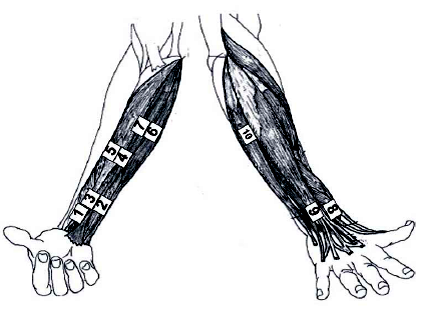
\includegraphics[width=6cm]{Shamonin2.png}
  \caption{Положение электродов при регистрации ЭМГ}
  \label{Shamonin2}

\end{figure}

\end{center}

Практическим методом была установлена взаимосвязь амплитуды получаемого сигнала на конкретном участке мышцы от степени сгибания пальцев руки.

В результате проверки выбранных методик измерения были получены 65\% и 95\% вероятности правильного определения сгибания пальца для 1-й и 2-й методик соответственно (рис. ~\ref{Shamonin3}). Время работы наиболее удовлетворительного алгоритма классификации составляет 0,5 мс, что позволяет применять его в режиме реального времени.
\begin{center}

\begin{figure}[h!]
  \centering
  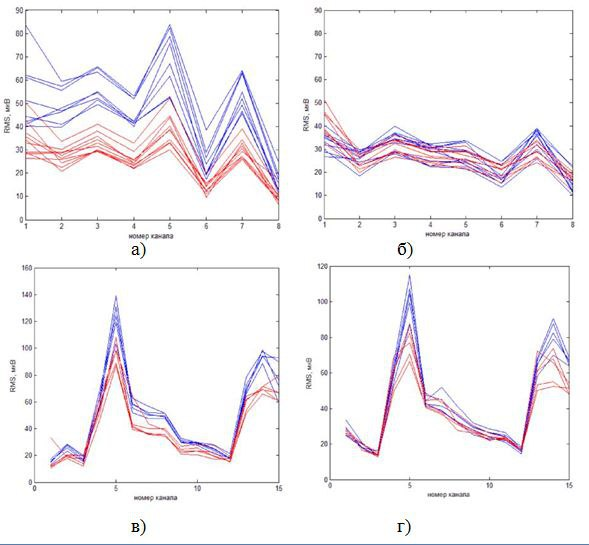
\includegraphics[width=8cm]{Shamonin3.jpg}
\caption{Примеры распознавания движений мизинца (а, в) и указательного пальца (б, г) в рамках 1-й (а, б) и 2-й (в, г) методик}
  
  \label{Shamonin3}

\end{figure}

\end{center}

\begin{thebibliography}{20}

\bibitem{shamonin-1} Muscle Sensor v3 Kit \url{https://www.sparkfun.com/products/retired/11776}

\end{thebibliography}

\end{document}

\documentclass[10pt, a5paper]{article}
\usepackage{pdfpages}
\usepackage{parallel}
\usepackage[T2A]{fontenc}
\usepackage{ucs}
\usepackage[utf8x]{inputenc}
\usepackage[polish,english,russian]{babel}
\usepackage{hyperref}
\usepackage{rotating}
\usepackage[inner=2cm,top=1.8cm,outer=2cm,bottom=2.3cm,nohead]{geometry}
\usepackage{listings}
\usepackage{graphicx}
\usepackage{wrapfig}
\usepackage{longtable}
\usepackage{indentfirst}
\usepackage{array}
\newcolumntype{P}[1]{>{\raggedright\arraybackslash}p{#1}}
\frenchspacing
\usepackage{fixltx2e} %text sub- and superscripts
\usepackage{icomma} % коскі ў матэматычным рэжыме
\PreloadUnicodePage{4}

\newcommand{\longpage}{\enlargethispage{\baselineskip}}
\newcommand{\shortpage}{\enlargethispage{-\baselineskip}}

\def\switchlang#1{\expandafter\csname switchlang#1\endcsname}
\def\switchlangbe{
\let\saverefname=\refname%
\def\refname{Літаратура}%
\def\figurename{Іл.}%
}
\def\switchlangen{
\let\saverefname=\refname%
\def\refname{References}%
\def\figurename{Fig.}%
}
\def\switchlangru{
\let\saverefname=\refname%
\let\savefigurename=\figurename%
\def\refname{Литература}%
\def\figurename{Рис.}%
}

\hyphenation{admi-ni-stra-tive}
\hyphenation{ex-pe-ri-ence}
\hyphenation{fle-xi-bi-li-ty}
\hyphenation{Py-thon}
\hyphenation{ma-the-ma-ti-cal}
\hyphenation{re-ported}
\hyphenation{imp-le-menta-tions}
\hyphenation{pro-vides}
\hyphenation{en-gi-neering}
\hyphenation{com-pa-ti-bi-li-ty}
\hyphenation{im-pos-sible}
\hyphenation{desk-top}
\hyphenation{elec-tro-nic}
\hyphenation{com-pa-ny}
\hyphenation{de-ve-lop-ment}
\hyphenation{de-ve-loping}
\hyphenation{de-ve-lop}
\hyphenation{da-ta-ba-se}
\hyphenation{plat-forms}
\hyphenation{or-ga-ni-za-tion}
\hyphenation{pro-gramming}
\hyphenation{in-stru-ments}
\hyphenation{Li-nux}
\hyphenation{sour-ce}
\hyphenation{en-vi-ron-ment}
\hyphenation{Te-le-pathy}
\hyphenation{Li-nux-ov-ka}
\hyphenation{Open-BSD}
\hyphenation{Free-BSD}
\hyphenation{men-ti-on-ed}
\hyphenation{app-li-ca-tion}

\def\progref!#1!{\texttt{#1}}
\renewcommand{\arraystretch}{2} %Іначай формулы ў матрыцы зліпаюцца з лініямі
\usepackage{array}

\def\interview #1 (#2), #3, #4, #5\par{

\section[#1, #3, #4]{#1 -- #3, #4}
\def\qname{LVEE}
\def\aname{#1}
\def\q ##1\par{{\noindent \bf \qname: ##1 }\par}
\def\a{{\noindent \bf \aname: } \def\qname{L}\def\aname{#2}}
}

\def\interview* #1 (#2), #3, #4, #5\par{

\section*{#1\\{\small\rm #3, #4. #5}}

\def\qname{LVEE}
\def\aname{#1}
\def\q ##1\par{{\noindent \bf \qname: ##1 }\par}
\def\a{{\noindent \bf \aname: } \def\qname{L}\def\aname{#2}}
}

\switchlang{ru}
\begin{document}
\title{Hubzilla --- введение, возможности, Hubzilla-сообщество \footnote{\url{tech@sprechrun.de} \url{http://lvee.org/ru/abstracts/244}}}
\author{Gustav Wall, Oldenburg(Oldb), Germany}
\maketitle
\begin{abstract}
Hubzilla is a free and open source platform running on a special kind of web server, called a <<hub>>, that can connect to other hubs in a decentralised network called <<the grid>>, providing sophisticated communications, identity, and access control services which work together seamlessly across domains and independent websites. It allows anybody to publicly or privately publish content via <<channels>>.
\end{abstract}
\subsection*{Что такое Хабзилла?}

%\begin{center}
%\begin{figure}[h!]
%  \centering
%  
\includegraphics[width=4cm]{Wall1.png}
  
%  \label{Wall_1}
%\end{figure}
%\end{center}

Hubzilla (Хабзилла, в дальнейшем Hbz) ~--- это платформа в форме децентральной сети, созданная с целью обеспечить возможность общения без цензуры и с соблюдением приватности. Сама структура Hubzilla сети и Hbz протокол Zot \footnote{\url{https://hub.libranet.de/help/developer/zot_protocol}} обеспечивают комфортное общение всех участников сети на равных. Hubzilla обладает многими полезными свойствами. Важность, значение каждого из этих свойств в каждом конкретном случае зависит от того, для каких целей вы используете это платформу.

\subsection*{Свойства, важные для всех ~--- вездесущность и доступность}

Два замечательных свойства Hbz понятны, важны и привлекательны для всех пользователей этой платформы ~--- вездесущность и доступность.

\textbf{вездесущность} в контексте Hbz это:

\begin{itemize}
  \item с одной стороны \emph{вездесущность в буквальном глобальном смысле}, т.е. способность и возможность для участников сети Hubzilla получить доступ и пользоваться сервисами этой сети везде, где участник или участница сети имеют возможность войти в свою учётную запись и контактировать своего виртуального \emph{кочующего двойника}. Неисправность одного из узлов не оказывает существенного влияния ни на работоспособность отдельных участников сети, ни на работоспособность сети в целом.
  \item вездесущность в смысле возможности \emph{с небольшими затратами времени обменивать сообщения с большим количеством контактов}. Эта вездесущность обеспечивается за счёт того, что при вводе сообщения участники Hbz-сети простым вводом символа \textbf{@(собака)} с последующим вводом какой-нибудь буквы или нескольких букв могут показать \textbf{все контакты}, содержащие введённую последовательность символов. Такой контакт может быть и рассылкой. Каждый подписчик рассылки может получить сообщение без того, что отправитель и получатель до этого общались.
\end{itemize}

Необычно \textbf{высокие значения доступности сервисов} в смысле ITIL \footnote{\url{https://itsm365.ru/blog/upravlenie-dostupnostyu-availability-management-po-itil/}} являются ещё одним уникальным свойством Hbz сети и достигается благодаря вездесущности его участников. Доступность самой сети и вездесущность её участников ~--- это две стороны одной медали. В сети Hbz доступность, стабильность сети растёт пропорционально с увеличением количества её участников.

\subsection*{Кочующий двойник и другие удобства}

\textbf{Кочующий двойник} является одним из центральных понятий в Hbz-сети, которое позволяет реализовать в сети эффект вездесущности. Уникальное свойство  вездесущности возможно благодаря тому, что участники могут на своё усмотрение с согласия оператора узла размещать свою учётную запись параллельно на разных узлах сети, удалять эту запись, что приводит к \textbf{повышению надёжности доступа к учётной записи практически до 100\%}. Если участник изменит данные на одном из узлов, обновляются данные и на узлах-двойниках. Непрерывно в режиме реального времени двойники обменивают данные, благодаря чему любой из двойников постоянно знает то, что знает и его протагонист.

\subsection*{Доступно по умолчанию}

Следующими возможностями могут пользоваться владельцы узла после установки Hbz \textbf{по умолчанию}:

\begin{itemize}
  \item адресная книга (контакты)
  \item сайт, веб-ресурс
  \item социальные сети
  \item форумы
  \item календарь мероприятий
  \item вики
  \item чат
  \item облачное хранилище файлов
  \item набор приложений (apps), который может расширяться в соответствии с потребностями владельца узла.
\end{itemize}

Обмен сообщениями в сети производится в соответствии с https-протоколом. Дополнительно имеется возможность закодировать часть или всё сообщение паролем.

\subsection*{Многосторонне одарённый двойник}

\textbf{Общительность} --- способность обменивать сообщения с другими сетями, например такими как Диаспора\footnote{\url{https://ru.wikipedia.org/wiki/Diaspora}} или Фриндика\footnote{\url{https://ru.wikipedia.org/wiki/Friendica}}.

\textbf{Всеядность} ~--- способность переваривать, интегрировать множество форматов ~--- \emph{HTML}, простой текст, \emph{bbcode, markdown, application/x-php}, благодаря чему пользователи могут в своих сообщениях комбинировать содержимое из разных источников с малыми затратами времени.

\textbf{Универсальность, неприхотливость} ~--- в зависимости от нагрузки на конкретном узле Hbz, зависящей от количества зарегистрированных пользователей, от активности, в том числе от количества контактов этих пользователей и от количества посетителей на узле можно установить этот узел на соответствующем железе ~--- Hbz работает на мини-компьютере Raspberry Pi \footnote{\url{https://www.raspberrypi.org/}} так же надёжно, как на сервере с мощнейшими AMD- или Intel-Xeon- мультипроцессорами.

\subsection*{Виртуальный кабинет ~--- рабочее место двойника}

Zot ~--- это \footnote{\url{https://hub.libranet.de/help/developer/zot_protocol}} специальный протокол, который обеспечивает обмен информацией, управление двойниками и управление доступом в децентральной сети, состоящей из независимых узлов (hubs). Эту сеть в Hbz-контексте часто называют грид (grid). Hbz-узлы выполняют различные функции, важнейшие из которых для владельца узла:

\begin{itemize}
  \item предоставление \textbf{виртуального кабинета} \emph{кочующему двойнику} владельца узла, который имеет в своём распоряжении:
  \begin{itemize}
	  \item контакты владельца узла
	  \item место встречи с другими двойниками
	  \item своего рода \textbf{передающую станцию} с одним или множеством каналов или \textbf{издательство} с одним или множеством изданий
	  \item систему для \textbf{прецизионного управления доступом} к каждому из объектов на узле
  \end{itemize}
  \item двойник в соответствии с доверенными ему полномочиями выполняет массу дел, связанных с общением с другими двойниками из сети Hbz или с гостями сети
  \item практически неограниченное количество принадлежащих владельцу узла \textbf{виртуальных кабинетов}, куда он может пустить как \emph{постояльцев} чужих двойников:
	\begin{itemize}
	  	\item каждый из чужих двойников имеет в своём распоряжении практически те же возможности, что двойник владельца узла, особенно если постоялец и владелец доверяют друг другу или они заключили соответствующий договор о найме виртуального кабинета.
	\end{itemize}
\end{itemize}

Таким образом сеть Hbz представляет собой пространство, среду обитания для двойников, объём полномочий которых предопределяется оригиналом.

\subsection*{Возможности применения}

Картинки отображают образно или схематично возможные сценарии применения Hbz. MicroSD отображает тот факт, что сервер Hubzilla можно установить на этой карте размером с ноготок.

\begin{center}
\begin{figure}[h!]
  \centering
  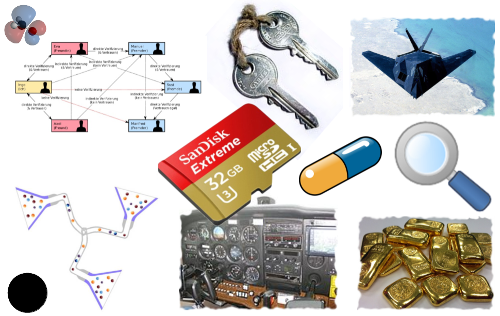
\includegraphics[width=4cm]{Wall2.png}
  
  \label{Wall2}
\end{figure}
\end{center} 

\begin{thebibliography}{20}
\bibitem{Wall-1} Hubzilla помощь ~--- \url{http://hub2.sprechrun.de/help/}
\bibitem{Wall-2} The history of Hubzilla ~--- \url{http://www.talkplus.org/blog/2016/the-history-of-hubzilla/}
\bibitem{Wall-3} Аккаунт, двойник автора (Gustav Wall) в сети Хабзилла ~--- \url{https://\%hub.libranet.de/channel/nmoplus}
\bibitem{Wall-4} Web of Trust Von \url{https://commons.wikimedia.org/wiki/User/Ogmios} ~--- \url{https://upload.wikimedia.org/wikipedia/commons} ~--- \url{https://upload.wikimedia.org/wikipedia/commons/4/4e/Web\_of\_Trust.svg, CC BY-SA 3.0}, \url{https://commons.wikimedia.org/w/index.php?curid=30127548}
\bibitem{Wall-5} Zwei gleiche Schlüssel Von Sebastian Hartlaub ~--- Eigenes Werk, CC BY-SA 3.0, \url{https://commons.wikimedia.org/w/index.php?curid=696513}
\end{thebibliography} 

\end{document}

\documentclass[10pt, a5paper]{article}
\usepackage{pdfpages}
\usepackage{parallel}
\usepackage[T2A]{fontenc}
\usepackage{ucs}
\usepackage[utf8x]{inputenc}
\usepackage[polish,english,russian]{babel}
\usepackage{hyperref}
\usepackage{rotating}
\usepackage[inner=2cm,top=1.8cm,outer=2cm,bottom=2.3cm,nohead]{geometry}
\usepackage{listings}
\usepackage{graphicx}
\usepackage{wrapfig}
\usepackage{longtable}
\usepackage{indentfirst}
\usepackage{array}
\newcolumntype{P}[1]{>{\raggedright\arraybackslash}p{#1}}
\frenchspacing
\usepackage{fixltx2e} %text sub- and superscripts
\usepackage{icomma} % коскі ў матэматычным рэжыме
\PreloadUnicodePage{4}

\newcommand{\longpage}{\enlargethispage{\baselineskip}}
\newcommand{\shortpage}{\enlargethispage{-\baselineskip}}

\def\switchlang#1{\expandafter\csname switchlang#1\endcsname}
\def\switchlangbe{
\let\saverefname=\refname%
\def\refname{Літаратура}%
\def\figurename{Іл.}%
}
\def\switchlangen{
\let\saverefname=\refname%
\def\refname{References}%
\def\figurename{Fig.}%
}
\def\switchlangru{
\let\saverefname=\refname%
\let\savefigurename=\figurename%
\def\refname{Литература}%
\def\figurename{Рис.}%
}

\hyphenation{admi-ni-stra-tive}
\hyphenation{ex-pe-ri-ence}
\hyphenation{fle-xi-bi-li-ty}
\hyphenation{Py-thon}
\hyphenation{ma-the-ma-ti-cal}
\hyphenation{re-ported}
\hyphenation{imp-le-menta-tions}
\hyphenation{pro-vides}
\hyphenation{en-gi-neering}
\hyphenation{com-pa-ti-bi-li-ty}
\hyphenation{im-pos-sible}
\hyphenation{desk-top}
\hyphenation{elec-tro-nic}
\hyphenation{com-pa-ny}
\hyphenation{de-ve-lop-ment}
\hyphenation{de-ve-loping}
\hyphenation{de-ve-lop}
\hyphenation{da-ta-ba-se}
\hyphenation{plat-forms}
\hyphenation{or-ga-ni-za-tion}
\hyphenation{pro-gramming}
\hyphenation{in-stru-ments}
\hyphenation{Li-nux}
\hyphenation{sour-ce}
\hyphenation{en-vi-ron-ment}
\hyphenation{Te-le-pathy}
\hyphenation{Li-nux-ov-ka}
\hyphenation{Open-BSD}
\hyphenation{Free-BSD}
\hyphenation{men-ti-on-ed}
\hyphenation{app-li-ca-tion}

\def\progref!#1!{\texttt{#1}}
\renewcommand{\arraystretch}{2} %Іначай формулы ў матрыцы зліпаюцца з лініямі
\usepackage{array}

\def\interview #1 (#2), #3, #4, #5\par{

\section[#1, #3, #4]{#1 -- #3, #4}
\def\qname{LVEE}
\def\aname{#1}
\def\q ##1\par{{\noindent \bf \qname: ##1 }\par}
\def\a{{\noindent \bf \aname: } \def\qname{L}\def\aname{#2}}
}

\def\interview* #1 (#2), #3, #4, #5\par{

\section*{#1\\{\small\rm #3, #4. #5}}

\def\qname{LVEE}
\def\aname{#1}
\def\q ##1\par{{\noindent \bf \qname: ##1 }\par}
\def\a{{\noindent \bf \aname: } \def\qname{L}\def\aname{#2}}
}

\switchlang{be}
\begin{document}
\title{Бізнэс-мадэлі для супольнай уласнасці або як прадаваць атамы і не біты.\footnote{\url{fannrm@gmail.com} \url{http://lvee.org/ru/abstracts/253}}}
\author{Mikhail Volchak, Minsk, Belarus}
\maketitle
\begin{abstract}
In the presentation different business models based on the digital commons were summarized. The first point is a consideration who controls a modern pool of resources and which characteristics are critical for the resource management. In the second point we discuss how the digital revolution change price-creation of a digital content. Further we elaborate how to make money and foster development based on Creative Commons principles. The last section describes how businesses can operate based on non-market premises and develop the third way in the content creation, distribution and consumption.
\end{abstract}
Бізнэс мадэлі для супольнай уласнасці або як прадаваць атамы і не біты.

<<Кожны збытак стварае новы дыфіцыт>> 
(Свабодны, Андэрсан)

Найбольш частае пытанне, якое задаюць слухачы падчас лекцый і выступаў па тэме распаўсюду ідэй Creative Commons: як творчы чалавек можа зарабіць у Беларусі сабе на жыццё або стаць багатым выкарыстощваючы Creative Commons ліцэнзіі?

Перад тым як пачаць пералічваць што значыць быць зробленым творчым агульным, звернемся да асноўваў сучаснай палітэканоміі. Тут будзе палягаць частка адказу мета ўзроўню, а менавіта хто кіруе рэсурсамі.

\subsubsection*{Агульнае супольнае}

Гістарычна склалася 3 асноўных падыхода у кіраванні рэсурамі:

\begin{enumerate}
  \item Дзяржаўная манаполія, значыць, што урад кантралюе вытворчасць, размеркаванне і спажыванне рэсурсаў,
  \item Падыход рынкавых адносінаў кантралюе рэсурсы інстытутам прыватнай ўласнасці.
  \item Супольныя рэсурсы ~--- гэта значыць, што рэсурсы кантралююцца калектыўна, грамадзянамі.
\end{enumerate}

Доўгі час у Беларусі мы мелі сітуацыю, калі рынкавыя і грамадскія механізмы былі ўлучаны ў адзін ~--- дзяржаўны, і кантраляваліся урадам (або партыяй).

Апошнія 25 год незалежнасці Беларусь абрала рынкавы \linebreak механізм. У разуменні шляхоў развіцця замацавалася два асноўных падыхода. Першы кажа, пра тое, што дзяржава павінна кантраляваць рэсурсы і эканоміку, а другі прасоўвае свабодны рынак, які павінен выканаць функцыю мадэрнізатара эканомікі і жыцця грамадзян.

Але ў гэтай схеме ёсць недаацэненая кампанента ~--- грамадства. Якое прапаноўвае іншыя варыянт кіравання рэсурсамі у адрозненні ад дзяржаўнага або неаліберальнага капіталізма. Гэты падыход базуецца на ~--- супольным, або супольнай уласнасці.

Эліанор Острам выдзяляе асноўныя 4 кампаненты ў кіраванні рэсурсамі:

\begin{itemize}
  \item Характарыстыка рэсурсаў. Яны натуральныя або створаны чалавекам, іх дэфіцыт, або лішак, маюць фізічную або лічбавую аснову?
  \item Нормы і правілы. Што кантралюе рэсурсы: нефармальныя нормы, або фармальныя правілы ~--- законы?
  \item Людзі і працэсы. Хто мае доступ і можа карыстацца імі, хто мае ўладу над рэсурсамі, прамую або ўскосную?
  \item Мэты. Як карыстаецца здабытае, рэсурс пастаянна дадаецца (як вікіпедыя) або выймаецца (як нафта)?
\end{itemize}

У 1980-90х адбылася лічбавая рэвалюцыя і Столман з паплечнікамі аб’явілі 4 свабоды для эканомікі супольнага (або грамадскага набытку на падставе праватных дамоваў):

\begin{itemize}
  \item карыстацца праграмай;
  \item змяняць і вывучаць праграму;
  \item распаўсюджваць яе;
  \item распаўсюджваць у тым ліку змененыя копіі.
\end{itemize}

Гэты рух надалей стварыў перадумавы для лічбавага супольнага, у які была уключаны не толькі код, але і кантэнт.

Інтэрнет даў тры асноўныя магчымасці:

\begin{itemize}
  \item Прыблізіць кошто копіі амаль да нуля, што дае магчымасць неабмежаванага тыражу.
  \item І аўтарства стала ўніверсальнай з’явай дзе амаль кожны можа быць аўтарам і распаўсбджваць свой кантэнт, у тым ліку бясплатна.
  \item Што ў сваю чаргу стварыла новыя ўмовы для кіравання рэсурсамі. Дзе стваральнікі кантэнту канкуруюць не толькі з тымі, хто прадае кантэнт, але з аўтарамі, які распаўсюджвае яго бясплатна.
\end{itemize}

Такім чынам, аўтараў, якія жадаюць прытрымлівацца супольнага падыходу да кіравання рэсурсамі стаіць няпростае пытанне: як захоўваючы каштоўнасць адкрытага доступа, да сваёй творчасці зарабіць грошы?

\subsubsection*{Што рабіць з нулявым коштам?}

Ніжэй прапанаваны падыходы сабраныя Пола Стэйсці і Сарай Персан з 24 пачынанняў які выкарысталі наступныя прынцыпы у сваіх бізнэс мадэлях:

\begin{itemize}
  \item Больш аўдыторыі. Creative Commons не ствараюць вірусны эффект, але яны ствараюць ўмовы для свабоднага распаўсюду. Тым самым правакуючы эффект далучэння да большасці.
  \item Прызнанне і рэпутацыя. Creative Commons механізмы патрабуюць пазначэнне аўтарства твораў, што з’яўляецца нормай для шматлікіх грамадстваў і супольнасцяў. Таким чынам \linebreak аўтарства як значны атрыбут для дадання вартасци творчаму прадукту.
  \item Раскрутка і прасоўванне. Электронная версія прадукт для прасоўвання, а фізічная як тавар, такім чынам эканомяцца грошы на рэкламу.
  \item Гуляць па сваіх правілах. Creative Commons дае магчымасць вызначаць свае правілы гульні і ўцягнення аўдыторыі, на рынку ў тым ліку.
  \item Сустварэнне. Creative Commons дае магчымасць перапрацоўваць творы і гэта ўключае спажыўцоў (напрыклад, мастакоў і музыкаў) у сумесную творчасць, тым самым павялічваючы сувязі з творамі.
\end{itemize}

\subsubsection*{Як зарабляць грошы?}

Галоўнае пытанне ў гэтай часцы, што ж cтварае дадатковую вартасць, за якую людзі гатовы плаціць?

Выкарыстоўваючы стандартныя рынкавыя мезанізмы:

Прадастаўленне кастамізаванага сэрвіса. Кантэнту бясплатнага шмат, але, каб атрымаць патрэбны толькі сабе кантэнт, неабходна заплаціць.
Прадастаўленне фізічнай копіі. Электроная копія бясплатна, але фізічная рэалізацыя за грошы. Напрыклад, дызайн мэблі або электронікі.

\begin{itemize}
  \item Аплата за персанізаваную версію. Персанальны досвед творчасці. Напрыклад, канцэрт, або лекцыя.
  \item Продаж свэга і мерчэндайза. Цішоткі і т.п.
  \item Сбор грошай з рэкламадаўца і спонсараў. Традыцыйны падыход.
  \item Стваральнікі кантэнта аплочваюць месца. Напрыклад, платформа навуковых артыкулаў.
  \item Аплата транзакцый. Напрыклад, платформа, на якой узаемадзенічаюць кліенты і творцы.
  \item Аплата прыладаў. Платформы збіраюць грошы за выкарыстанне прасунутых інструментаў.
  \item Выкарыстанне брэнда. Напрыклад, брэнда, які асацыюецца з пэўнай якасцю, накірункам, даверам.
\end{itemize}

Але ёсць накірунак, які больш факусуецца на не рынкавых механізмах, а на ўзаемнасці:

\begin{itemize}
  \item Сяброўскія ўнёскі або інтывідуальныя ахвяраванні. Чым \linebreak больш  тых, хто атрымлівае дадатковую вартасць, тым больш тых, хто верагодна можа падтрымаць праект.
  \item Свабодны кошт. Карыстальнікі плоцяць столькі колькі пажадаюць, як акт удзячнасці.
  \item Краўдфандынг. Вырошчванне супольнасці для таго, каб яна не толькі падтрымала, але і хацела поспеха праекту.
\end{itemize}

\subsubsection*{Злучаць людзей}

Акрамя выкарыстання Creative Commons, як прававога інструмента, з’яўляецца сродкам нагадвання, што за кожным творам стаіць чалавек, тым самым? ствараючы пачуццё абавязку. Далей пералічана шэраг ідэй, якія выкарыстоўваюцца ў новых бізнэс мадэлях:

\begin{itemize}
  \item Расказаваць гісторыі творчасці і не баяцца крытыкі, каманда не лашчоны брэнд.
  \item Адкрытасць да камунікацыі і адказнасць. Адказнасць ~--- не значыць канфармізм, а магчымасць аўдыторыі ведаць рашэнні і падставы.
  \item Далёка не ўсё людзі прымаюць рашэнне на падставе эканамічнай выгады і эгаізма. Напрыклад, шмат хто цэніць магчымасць папрацаваць разам або давер адзін да аднаго.
  \item Разглядаць людзей як індывідаў. Гэта значыць прамыя кантакты стваральніка і карыстальніка/фаната.
  \item Публічна заяўляўленне сваіх прынцыпаў. Выражэнне каштоўнасцяў павінна быць яўным, не хаваючы іх.
  \item Будаваць супольнасць. Ствараць практыку патрэбнасці і прыналежнасці да супольнай працы, і стварэння агульнага адзінадумцамі. Супольнасць забірае сілы, але аб’ядноўвае высілкі.
  \item Шэрынг ~--- значыць, даваць больш, чым браць. Адкрыты кантэнт ~--- гэта не поле халяўных рэсурсаў, і не проста постынг свайго кантэнта, але дадатковая вартасць.Напрыклад, пэўная культура зносінаў або падтрымкі ўдзельнікаў.
  \item Уключаць людзей у тое, што робіш. Малыя ўнёскі найбольш значныя.
\end{itemize}

Статыстыка паказвае, што ў свеце існуе больш за 1.4 міл’ярда твораў пад СС. Гэта насамрэч ураджваючая з’ява сведчыць пра наяўнасць сусветнай супольнасці, якая папаўняе менавіта “лічбавае супольнае”, як альтэрнатыўны шлях эканамічнага, культурнага і сацыяльнага развіцця двум крайнасцям: дзяржаўнай або рынкавай манаполіі ў кіраванні рэсурсамі.

\begin{thebibliography}{99}

\bibitem{Volchak1} Paul Stacey, The new world of digital commons, 2017 (Book. Made Wi creative Commons)
\bibitem{Volchak2} Sarah Pearson, How to be made with creative commons, 2017 (Book. Made Wh creative Commons)
 \bibitem{Volchak3} Report. State of the commons, 2016 ~--- \url{https://stateof.creativecommons.org/}
\end{thebibliography}

\end{document}

\documentclass[10pt, a5paper]{article}
\usepackage{pdfpages}
\usepackage{parallel}
\usepackage[T2A]{fontenc}
\usepackage{ucs}
\usepackage[utf8x]{inputenc}
\usepackage[polish,english,russian]{babel}
\usepackage{hyperref}
\usepackage{rotating}
\usepackage[inner=2cm,top=1.8cm,outer=2cm,bottom=2.3cm,nohead]{geometry}
\usepackage{listings}
\usepackage{graphicx}
\usepackage{wrapfig}
\usepackage{longtable}
\usepackage{indentfirst}
\usepackage{array}
\newcolumntype{P}[1]{>{\raggedright\arraybackslash}p{#1}}
\frenchspacing
\usepackage{fixltx2e} %text sub- and superscripts
\usepackage{icomma} % коскі ў матэматычным рэжыме
\PreloadUnicodePage{4}

\newcommand{\longpage}{\enlargethispage{\baselineskip}}
\newcommand{\shortpage}{\enlargethispage{-\baselineskip}}

\def\switchlang#1{\expandafter\csname switchlang#1\endcsname}
\def\switchlangbe{
\let\saverefname=\refname%
\def\refname{Літаратура}%
\def\figurename{Іл.}%
}
\def\switchlangen{
\let\saverefname=\refname%
\def\refname{References}%
\def\figurename{Fig.}%
}
\def\switchlangru{
\let\saverefname=\refname%
\let\savefigurename=\figurename%
\def\refname{Литература}%
\def\figurename{Рис.}%
}

\hyphenation{admi-ni-stra-tive}
\hyphenation{ex-pe-ri-ence}
\hyphenation{fle-xi-bi-li-ty}
\hyphenation{Py-thon}
\hyphenation{ma-the-ma-ti-cal}
\hyphenation{re-ported}
\hyphenation{imp-le-menta-tions}
\hyphenation{pro-vides}
\hyphenation{en-gi-neering}
\hyphenation{com-pa-ti-bi-li-ty}
\hyphenation{im-pos-sible}
\hyphenation{desk-top}
\hyphenation{elec-tro-nic}
\hyphenation{com-pa-ny}
\hyphenation{de-ve-lop-ment}
\hyphenation{de-ve-loping}
\hyphenation{de-ve-lop}
\hyphenation{da-ta-ba-se}
\hyphenation{plat-forms}
\hyphenation{or-ga-ni-za-tion}
\hyphenation{pro-gramming}
\hyphenation{in-stru-ments}
\hyphenation{Li-nux}
\hyphenation{sour-ce}
\hyphenation{en-vi-ron-ment}
\hyphenation{Te-le-pathy}
\hyphenation{Li-nux-ov-ka}
\hyphenation{Open-BSD}
\hyphenation{Free-BSD}
\hyphenation{men-ti-on-ed}
\hyphenation{app-li-ca-tion}

\def\progref!#1!{\texttt{#1}}
\renewcommand{\arraystretch}{2} %Іначай формулы ў матрыцы зліпаюцца з лініямі
\usepackage{array}

\def\interview #1 (#2), #3, #4, #5\par{

\section[#1, #3, #4]{#1 -- #3, #4}
\def\qname{LVEE}
\def\aname{#1}
\def\q ##1\par{{\noindent \bf \qname: ##1 }\par}
\def\a{{\noindent \bf \aname: } \def\qname{L}\def\aname{#2}}
}

\def\interview* #1 (#2), #3, #4, #5\par{

\section*{#1\\{\small\rm #3, #4. #5}}

\def\qname{LVEE}
\def\aname{#1}
\def\q ##1\par{{\noindent \bf \qname: ##1 }\par}
\def\a{{\noindent \bf \aname: } \def\qname{L}\def\aname{#2}}
}

\switchlang{be}
\begin{document}
\title{Адкрытыя графічныя прылады Gimp і InkScape. Плюсы і мінусы\footnote{\url{imfantina@gmail.com}, \url{http://lvee.org/ru/abstracts/239}}}
\author{Святлана Ермаковіч, Minsk, Belarus}
\maketitle
\begin{abstract}
Comparison of the basic functions and particular tasks is done for free/libre (Gimp, InkScape) and non-free (Photoshop, CorelDraw) graphic editors from the amateur designer point of view. Things which were successfully performed with use of FLOSS are listed as far as those which weren't. Also disadvantages are classified along their severity. 
\end{abstract}
Свабодныя графічныя прылады Gimp і InkScape адрозніваюцца ад сваіх прапрыетарных аналагаў (возмем, Photoshop і CorelDraw). Параўнаем асноўныя функцыі і частыя задачы свабодных і несвабодных прыладаў на ўзроўні аматару дызайну.

\subsection*{Графічныя заданні і асноўныя функцыі}

\subsubsection*{\textbf{Gimp vs Photoshop}}

\subsubsection*{Карэкцыя фотаздымкаў.}

Асноўныя функцыі карэкцыі: яркасць, кантраснасць, баланс колераў, адценне, насычанасць і іншыя есць у дзвюх прыладах.
Крыху адрозніваюцца алгарытмы гэтых функцый. І таму рэзультат прымянення адной і тойжа можа быць розны.

\subsubsection*{Калаж: праца са слаямі, выдаленне фону, змена памераў, абрэзка.}

\textbf{Абрэзка фону.} У Gimp ёсць функцыі як выдзялення аднаго і таго ж колеру ўсюды, так і <<магічная палачка>>, якая выдзяляе некае адценне ў інтэрвале колера. Інтэрвал можна задаваць. Зручна для апрацоўцы сфатаграфаваных або адсканаваных малюнкаў.
У Photoshop есць <<магічная палачка>> таксама.

\textbf{Змена памераў.} У Gimp існуе асобная кнопка на панэлі. У Photoshop ~--- гэта <<гарачая кнопка>> Ctrl+T, узгадаць дзе знаходзіцца аналагічная функцыя ў панэлях прыладаў пакуль неўдалося.

\textbf{Праца са слаямі.} У Gimp трэба крыху прызвычаецца да \linebreak ўстаўкі малюнка на новы слой, бо ен дадаецца не аўтаматычна (як пры выбары слою ў Photoshop), а на віртуальны слой, які неабходна зафіксаваць асобнай кнопкай на выбраны.
Функцыі бачнасці-нябачнасці, перасоўвання слаёў, склейкі, капіравання, рэгулявання празрыстасці таксама існуюць у Gimp. Аднак склейка адбываецца не паміж абранымі слаямі (як у Photoshop), апаміж суседнімі (верхні склеіваецца з ніжнім).

\textbf{Абрэзка.} У Gimp магчыма адразу змяняць памер поля абрэзкі пасля выдзялення. У Photoshop памер выдзялення можна змяняць праз меню правай кнопкі. У абедзвюх прыладах есць <<разумная абрэзка>>, калі малюнак абразаецца па контару.

\subsubsection*{Маляванне з нуля}

Тут па сутнасці часта выкарыстоўваюцца вышэй азначаныя \linebreak функцыі: праца са слаямі, праца з пэнзлікамі і колерамі. У дзвюх прыладах можна лёгка змяняць як колеры (асноўны і колер фона), памеры і віды пэнзлікаў, празрыстаць слаёў.
Таксама часта ўжываюцца кнопкі <<размыцця>>, <<асвятлення>> і <<зацямнення>>. Апошнія дзве прадстаўлены ў Gimp адной кнопкай з магчымасцю выбару дакладный функцыі, а ў Photoshop ~--- дзвюма асобнымі кнопкамі.

\subsubsection*{Праца з тэкстам.}

У Photoshop праца з тэкстам зручней: ён легка маштабіруецца (як малюнак), захоўваючы свойствы. У Gimp мяняць памер тэкста можна толькі змяняя яго ў адзінках шрыфта (напрыклад у пойнтах, і толькі ў адпаведным для гэтага полі). Маштабаваць тэкст як малюнак можна таксама, але пры гэтым тэкст пераўтвараецца ў малюнак.

Перасоўваць тэкст ў Photoshop можна абраўшы слой, на якім знаходзіцца тэкст.
Перасованне ў Gimp тэксту (і іншых малюнкаў, якія складаюцца з контураў) выконваецца толькі калі трапіць курсорам менавіта на патрэбны тэкст (не на прабелы і пустыя месцы), ці з дапамогай клавішы <<shift>>.

\subsubsection*{Экспарт}

У Photoshop  функцыя <<захаваць як>> прапаноўвае выбар фармату захоўвання.
У Gimp <<захаваць як>> ~--- гэта захоўванне толькі ў фармаце .xcf, а каб захаваць у іншых фарматах неабходна карыстацца функцыяй <<экспартаваць як>>.



\subsubsection*{\textbf{InkScape vs CorelDraw}}

\subsubsection*{Крывыя Без’е}

У дзвюх прыладах прадстаўлены як крывыя Без’е, так і іншыя крывыя. Намаляваныя контуры можна рэдагаваць змяняючы вузлавыя кропкі, з якіх складаецца малюнак.

\subsubsection*{Трасіроўка}

Алгарытмы трасіроўкі ў InkScape і CorelDraw па-змоўчанню розныя. У CorelDraw малюнак разбіваецца на кавалкі, адмалёваныя ў вектары (нібыта пазл).
У InkScape малюнак трасіруецца на колькасць слаёў, якую можна задаць. Калі слаеў больш за 5-7 малюнак ужо вельмі цяжка рэдагаваць. І бывае, што лягчэй адмаляваць яго наноў у вектары.

\subsubsection*{Функцыі логікі.}

Union, difference, intersection, exclusion, division ~--- ёсць у дзвюх прыладах. (У CorelDraw яны больш інтуітыўныя).
Функцыя абрэзкі сваеасабліва рэалізавана ў кожнай з іх. Пад абрэзкай я маю на ўвазе, што ў вас есць малюнак (вектарны, ці растравы) і вам трэба вырэзаць з яго адмысловую форму.
Калі гэта форма ~--- прамавугольнік, то ў CorelDraw такая абрэзка робіцца кнопкай з лязом. А калі форма праізвольная, то праз функцыю змяшчэння вашага малюнка у кантэйнер формы.
У InkScape не важна якую форму трэба вырэзаць ~--- выконваецца функцыя абрэзкі (з малюнка знізу выразаецца форма, што зверху).

\subsubsection*{Праца з тэкстам, вёрстка}

Праца з тэкстам у дзвюх прыладах даволі зручная. Галоўнае не забываць пераводзіць шрыфты ў крывыя пры экспарце і друку.

\subsubsection*{Градзіент.}

У CorelDraw праца з градзіентамі больш інтуітыўная, у InkScape трэба прызвычаецца да вакна працы з градзіентам і выбарам колераў для кропак пераходу і задання празрыстасці для іх.

\subsubsection*{Экспарт}

InkScape захоўвае ў папулярных фарматах .eps .svg, якія могуць быць адчыненыя і ў CorelDraw, ці іншых прыладах.
InkScape экспартуе толькі ў png, што бывае не зручна (часта png важаць болей за jpg).



\subsection*{Чаго не хапае свабодным прыладам?}

\begin{enumerate}
  \item У Gimp і InkScape адсутнічае пераўтварэнне і праца са CMYK гамай. Гэта не зручна для друку, бо скажаюцца некаторыя колеры.
  \item У InkScape адсутнічае праца з некалькімі старонкамі, што вельмі неабходна пры верстцы невялічкіх буклетаў і брашур.
  \item У Gimp адсутнічае задаванне сцэнароў (паслядоўнасці каманд, якія неабходна зрабіць з файлам).
  \item Імпарт з Photoshop у Gimp магчымы, але знікнуць некаторыя фільтры (функцыі), напрыклад, цень. Таксама пры імпарце губляецца дрэва тэчак для слаеў, слаі ўладкоўваюцца па парадку (Гэта не зручна пры стварэнні дызайна для сайта, дзе звычайна ствараецца дрэва тэчак для слаеў з рознымі элементамі).
Адваротны імпарт з Gimp у Photoshop немагчымы.
  \item Пры імпарце .svg з CorelDraw у InkScape, ці наадварот, вектарны малюнак можа скажацца. Бывае, што экспарт залежыць ад версіі як CorelDraw, так і InkScape.
\end{enumerate}

\end{document}

\documentclass[10pt, a5paper]{article}
\usepackage{pdfpages}
\usepackage{parallel}
\usepackage[T2A]{fontenc}
\usepackage{ucs}
\usepackage[utf8x]{inputenc}
\usepackage[polish,english,russian]{babel}
\usepackage{hyperref}
\usepackage{rotating}
\usepackage[inner=2cm,top=1.8cm,outer=2cm,bottom=2.3cm,nohead]{geometry}
\usepackage{listings}
\usepackage{graphicx}
\usepackage{wrapfig}
\usepackage{longtable}
\usepackage{indentfirst}
\usepackage{array}
\newcolumntype{P}[1]{>{\raggedright\arraybackslash}p{#1}}
\frenchspacing
\usepackage{fixltx2e} %text sub- and superscripts
\usepackage{icomma} % коскі ў матэматычным рэжыме
\PreloadUnicodePage{4}

\newcommand{\longpage}{\enlargethispage{\baselineskip}}
\newcommand{\shortpage}{\enlargethispage{-\baselineskip}}

\def\switchlang#1{\expandafter\csname switchlang#1\endcsname}
\def\switchlangbe{
\let\saverefname=\refname%
\def\refname{Літаратура}%
\def\figurename{Іл.}%
}
\def\switchlangen{
\let\saverefname=\refname%
\def\refname{References}%
\def\figurename{Fig.}%
}
\def\switchlangru{
\let\saverefname=\refname%
\let\savefigurename=\figurename%
\def\refname{Литература}%
\def\figurename{Рис.}%
}

\hyphenation{admi-ni-stra-tive}
\hyphenation{ex-pe-ri-ence}
\hyphenation{fle-xi-bi-li-ty}
\hyphenation{Py-thon}
\hyphenation{ma-the-ma-ti-cal}
\hyphenation{re-ported}
\hyphenation{imp-le-menta-tions}
\hyphenation{pro-vides}
\hyphenation{en-gi-neering}
\hyphenation{com-pa-ti-bi-li-ty}
\hyphenation{im-pos-sible}
\hyphenation{desk-top}
\hyphenation{elec-tro-nic}
\hyphenation{com-pa-ny}
\hyphenation{de-ve-lop-ment}
\hyphenation{de-ve-loping}
\hyphenation{de-ve-lop}
\hyphenation{da-ta-ba-se}
\hyphenation{plat-forms}
\hyphenation{or-ga-ni-za-tion}
\hyphenation{pro-gramming}
\hyphenation{in-stru-ments}
\hyphenation{Li-nux}
\hyphenation{sour-ce}
\hyphenation{en-vi-ron-ment}
\hyphenation{Te-le-pathy}
\hyphenation{Li-nux-ov-ka}
\hyphenation{Open-BSD}
\hyphenation{Free-BSD}
\hyphenation{men-ti-on-ed}
\hyphenation{app-li-ca-tion}

\def\progref!#1!{\texttt{#1}}
\renewcommand{\arraystretch}{2} %Іначай формулы ў матрыцы зліпаюцца з лініямі
\usepackage{array}

\def\interview #1 (#2), #3, #4, #5\par{

\section[#1, #3, #4]{#1 -- #3, #4}
\def\qname{LVEE}
\def\aname{#1}
\def\q ##1\par{{\noindent \bf \qname: ##1 }\par}
\def\a{{\noindent \bf \aname: } \def\qname{L}\def\aname{#2}}
}

\def\interview* #1 (#2), #3, #4, #5\par{

\section*{#1\\{\small\rm #3, #4. #5}}

\def\qname{LVEE}
\def\aname{#1}
\def\q ##1\par{{\noindent \bf \qname: ##1 }\par}
\def\a{{\noindent \bf \aname: } \def\qname{L}\def\aname{#2}}
}

\switchlang{ru}
\begin{document}
\title{Картографический сервис на OpenSource - доступная картография каждому}
\author{Дмитрий Степанов, Минск, Belarus}
\maketitle
\begin{abstract}
In the modern world, geoinformation technologies are widely represented in the life of both individuals and companies as a whole. These are navigation systems, transport monitoring systems and many-sided programs and applications that use spatial information mapping on a cartographic basis. Modernity as a period is an era of commercial development of GIS \linebreak(geoinformation systems), expansion of the field of their application through integration with DBMS, the emergence of network applications - all this has opened the way for systems that support corporate and distributed geodatabases. This pushed development of not only commercial geoinformation systems but also freely \linebreak distributed products (QGIS, NextGISWEB, MapServer and others).
\end{abstract}
— Где карта, Билли? Нам нужна карта… 
— Какая карта?! У меня нет никакой карты!
— Где карта?!
(мультфильм <<Остров сокровищ>>, 1988)

\subsection*{Введение.}

В современном мире геоинформационные технологии повседневно присутствуют в жизни как персонально каждого человека, так и компаний в целом. Это навигационные системы, системы мониторинга транспорта и многоликие программы и приложения, использующие отображение пространственной информации на картографической основе. 
Современность как период ~--- это эра коммерческого развития ГИС (геоинформационных систем), расширение области их применения за счет интеграции с СУБД, появление сетевых приложений ~--- и все это открыло путь системам, поддерживающим корпоративные и распределенные базы геоданных.  Это стало толчком к развитию не только комерческих геоинформационных систем, но и свободно распространяемых продуктов.

\subsection*{Постановка задачи.}

В одной «мифической» компании как-то заметили, что хотя в названии у них есть слово геоинформационные технологии, но услуг, да и собственно  геоинформационных технологий, нет. Руководители компании нашли на стороне инженеров и поставили задачу реализовать собственную геоинформационную систему (ГИС) на свободно-распространяемом программном обеспечении, не ввязываясь в дорогостоящий процесс собственно разработки продукта.

Функционал решения должен включать:

\begin{itemize}
  \item возможность развития системы как продукта
  \item возможность интеграции решения в существующие собственные программные комплексы организации
  \item возможность публиковать собственные карты и картографические основы
  \item возможность реализовывать слои на картографической основе
  \item система должна быть проста в эксплуатации, дабы не содержать дорогостоящий персонал, для использования функционала продукта и в случае продажи не услуги, а собственно программного решения, то есть ГИС.
\end{itemize}

\subsection*{Выбор решения.}

Проведя анализ предлагаемых ГИС-платформ на проприетарной основе и определившись с тем, что бы хотелось получить в итоге, мы принялись за работу.

\subsection*{Что понадобиться?}

Картографическая основа. По причине отсутствия финансирования, а также из-за запрета эксплуатировать покупные карты, мы остановились на использовании собственного тайлового сервера, на картографической основе OSM (openstreetmap) ~\cite{Stepanov-7}. Популярность данной картографической подложки обусловлена,  во-первых, политикой предоставления тайлов, позволяющей любому желающему свободно использовать тайлы OpenStreetMap или иных картографических основ, разработанных на базе OSM в своих приложениях, а во-вторых, простотой их подключения в современных веб-клиентах, таких как Leaflet и OpenLayers.

Использование собственного сервера карт было обусловлено \linebreak необходимостью наличия картографической подложки при отсутствии доступа в общедоступным картам OSM, Яндекс Народная и т.п. Это позволяет, в случае необходимости реализовать проект без привязки к стороннему сервису картографической основы. В отдельных случаях вместо картографической основы можно использовать shape-слой,  созданный на основе картографической основы.

В качестве решения для создания печатных карт, а так же слоев пространственных данных, был выбран программный продукт QGIS ~\cite{Stepanov-1} (распространяемый по лицензии GNU General Public \linebreak License) ~--- как унифицированное решение с большим сообществом и соответственно поддержкой разносторонних модулей и мультиплатформенной архитектурой.

Серверов публикации данных было проанализировано несколько:

\begin{itemize}
  \item MapServer (на данный момент наверное самый популярный вариант сервера для публикации пространственных данных ~--- карт).
  \item QGIS Web Server (рассматривался исключительно из за высокого уровня совместимости с продуктом QGIS)
  \item NEXTGIS Web Server (Данное решение, было найдено случайно и как результат позволило получить максимальный результат)
\end{itemize}

По результатам изучения данного направления, был сделан выбор в пользу продукта от российской компании NEXTGIS: это обусловлено как распространением их решения по лицензии GNU GPL, так и тем, что они (собрав все описанные выше продукты) реализовали довольно интересный и функциональный продукт в <<коробочном>> исполнении, доступный для освоения обычным пользователям ~\cite{Stepanov-4}. Также подкупило наличие мобильных приложений (клиентов) для редактирования существующих слоев на веб-сервере и управления сервером с находясь <<в поле>>.

Что же касается QGIS Web Server ~\cite{Stepanov-5}, данное программное решение довольно простое в эксплуатации, но позволяет публиковать данные как демонстрацию слоя и карты, без конечного взаимодействия с объектами нанесенными на картографическую основу, что само по себе конечно уже много, но недостаточно для реализации поставленной задачи.

Отдельно хочется отметить продукт MapServer, так как он оказался структурообразующим продуктом и по сути присутствует в каждом из описанных выше решений. Это более чем гибкое решение для публикации пространственных данных на картографической основе, но реализация на нем слоев требует дополнительных знаний от конечного пользователя.

Пример создания mapfile для MapServer и слоя.

\begin{verbatim}
MAP
    NAME "sample"
    STATUS ON
    SIZE 600 400
    SYMBOLSET "../etc/symbols.txt"
    EXTENT -180 -90 180 90
    UNITS DD
    SHAPEPATH "../data"
    IMAGECOLOR 255 255 255
    FONTSET "../etc/fonts.txt"

    #
    # Start of web interface definition
    #
    WEB
        IMAGEPATH "/ms4w/tmp/ms_tmp/"
        IMAGEURL "/ms_tmp/"
    END # WEB

    #
    # Start of layer definitions
    #
    LAYER
        NAME 'global-raster
        TYPE RASTER
        STATUS DEFAULT
        DATA bluemarble.gif
    END # LAYER
 END # MAP
\end{verbatim}

\begin{center}

\begin{figure}[h!]
  \centering
  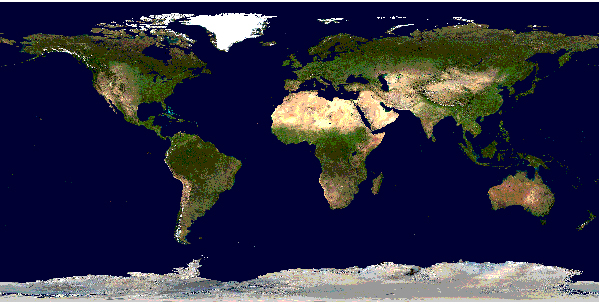
\includegraphics[width=10cm]{stepanov1.jpg}
  
  \label{Stepanov1}
\end{figure}

\end{center}


Для хранения пространственных данных большинство рассматриваемых свободно распространяемых продуктов использует СУБД PostgreSQL ~\cite{Stepanov-8}, а точнее, надстройку над СУБД ~--- PostGIS ~\cite{Stepanov-9}, позволяющую хранить в себе пространственные данные (точки, полигоны, линии и некоторые графические объекты).

\subsection*{Опыт использования в реальном проекте.}

\begin{itemize}
  \item Реализации проекта по созданию онлайн-ГИС для размещения культурных и туристических объектов Беларуси на картографической основе, доступной всем.
\begin{center}

\begin{figure}[h!]
  \centering
  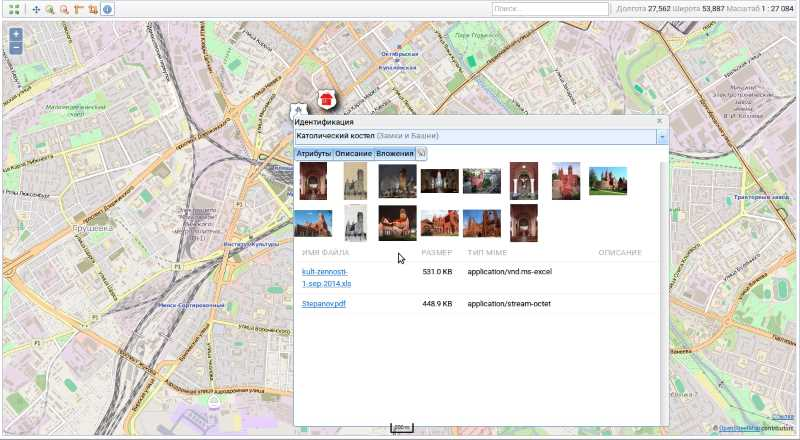
\includegraphics[width=10cm]{stepanov2.jpg}
  
  \label{Stepanov2}
\end{figure}
\begin{center}

\begin{figure}[h!]
  \centering
  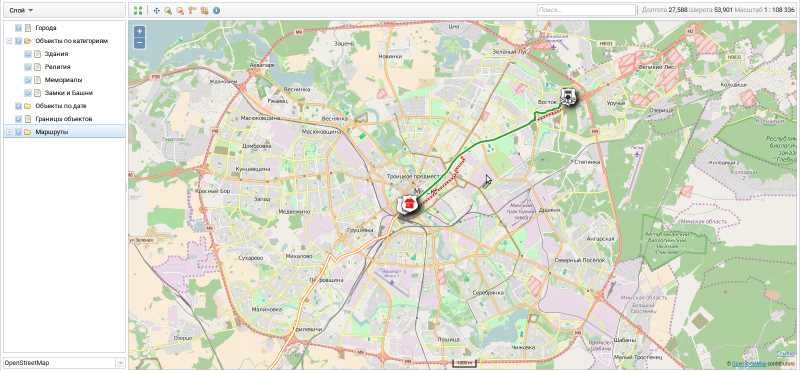
\includegraphics[width=10cm]{stepanov3.jpg}
  
  \label{Stepanov3}
\end{figure}

\end{center}

\end{center}


\end{itemize}

\begin{itemize}
  \item Отображение на картографической основе информации о работе светофоров с динамическим изменением стилистики отображаемого слоя.
  \item Отображение на картографической основе зон отношения к определенному гос. учреждению (милиция, поликлиника, \linebreak ЖЭС и т.д.v1)

\begin{center}

\begin{figure}[h!]
  \centering
  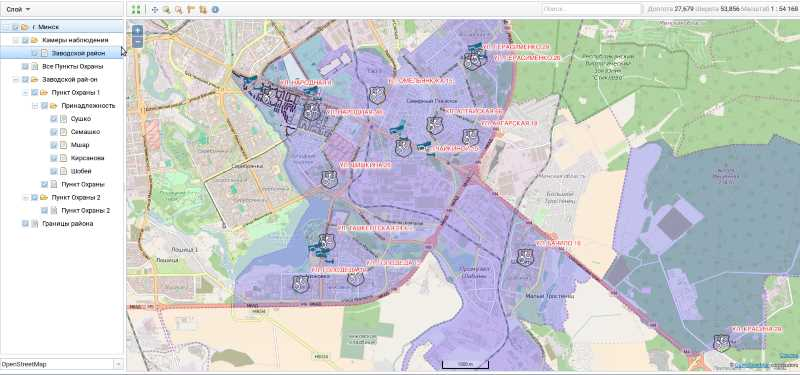
\includegraphics[width=10cm]{stepanov4.jpg}
  
  \label{Stepanov4}
\end{figure}

\end{center}

\end{itemize}

Подытожив, хочется воспользоваться цитатой из киносерии про пирата Джека Воробья:
 ~--- Да, раньше этот мир был куда больше\ldots{}
 ~--- Нет, мир остался прежним. Стало меньше содержимого.

\begin{thebibliography}{99}

\bibitem{Stepanov-1}Официальный портал продукта QGIS ~---  \url{http://qgis.org}{qgis.org}
\bibitem{Stepanov-2}Проект QGIS на гитхабе ~--- \url{https://github.com/qgis/QGIS}
\bibitem{Stepanov-3}Веб-клиент для работы с QGIS ~--- \url{https://github.com/qgis/QGIS-Web-Client}
\bibitem{Stepanov-4}Сайт продукта NEXTGISQGIS ~--- \url{http://nextgis.ru/nextgis-qgis/}
\bibitem{Stepanov-5}Реализация QGIS WEB Server ~--- \url{https://live.osgeo.org/ru/quickstart/qgis_mapserver_quickstart.html}
\bibitem{Stepanov-6}GIS-Lab ~--- неформальное сообщество специалистов в области ГИС и ДЗЗ ~--- \url{http://gis-lab.info/}
\bibitem{Stepanov-7}Ресурс картографической основы ~--- \url{http://www.openstreetmap.org}
\bibitem{Stepanov-8}СУБД ~--- \url{https://www.postgresql.org/}
\bibitem{Stepanov-9}Расширение для базы данных PostgreSQL ~---  \url{http://www.postgis.net/}
\bibitem{Stepanov-10}Проект NEXTGIS на гитхабе ~--- \url{https://github.com/nextgis}
\bibitem{Stepanov-11}Сайт продукта NEXTGIS ~--- \url{http://nextgis.ru/}
\bibitem{Stepanov-12}Проект NEXTGISWEB на гитхабе ~--- \url{https://github.com/nextgis/nextgisweb}
\bibitem{Stepanov-13}Интеграция публикации стилей слоев QGIS на NEXTGISWEB ~--- \url{https://github.com/nextgis/nextgisweb_qgis}
\end{thebibliography}

\end{document}

\documentclass[10pt, a5paper]{article}
\usepackage{pdfpages}
\usepackage{parallel}
\usepackage[T2A]{fontenc}
\usepackage{ucs}
\usepackage[utf8x]{inputenc}
\usepackage[polish,english,russian]{babel}
\usepackage{hyperref}
\usepackage{rotating}
\usepackage[inner=2cm,top=1.8cm,outer=2cm,bottom=2.3cm,nohead]{geometry}
\usepackage{listings}
\usepackage{graphicx}
\usepackage{wrapfig}
\usepackage{longtable}
\usepackage{indentfirst}
\usepackage{array}
\newcolumntype{P}[1]{>{\raggedright\arraybackslash}p{#1}}
\frenchspacing
\usepackage{fixltx2e} %text sub- and superscripts
\usepackage{icomma} % коскі ў матэматычным рэжыме
\PreloadUnicodePage{4}

\newcommand{\longpage}{\enlargethispage{\baselineskip}}
\newcommand{\shortpage}{\enlargethispage{-\baselineskip}}

\def\switchlang#1{\expandafter\csname switchlang#1\endcsname}
\def\switchlangbe{
\let\saverefname=\refname%
\def\refname{Літаратура}%
\def\figurename{Іл.}%
}
\def\switchlangen{
\let\saverefname=\refname%
\def\refname{References}%
\def\figurename{Fig.}%
}
\def\switchlangru{
\let\saverefname=\refname%
\let\savefigurename=\figurename%
\def\refname{Литература}%
\def\figurename{Рис.}%
}

\hyphenation{admi-ni-stra-tive}
\hyphenation{ex-pe-ri-ence}
\hyphenation{fle-xi-bi-li-ty}
\hyphenation{Py-thon}
\hyphenation{ma-the-ma-ti-cal}
\hyphenation{re-ported}
\hyphenation{imp-le-menta-tions}
\hyphenation{pro-vides}
\hyphenation{en-gi-neering}
\hyphenation{com-pa-ti-bi-li-ty}
\hyphenation{im-pos-sible}
\hyphenation{desk-top}
\hyphenation{elec-tro-nic}
\hyphenation{com-pa-ny}
\hyphenation{de-ve-lop-ment}
\hyphenation{de-ve-loping}
\hyphenation{de-ve-lop}
\hyphenation{da-ta-ba-se}
\hyphenation{plat-forms}
\hyphenation{or-ga-ni-za-tion}
\hyphenation{pro-gramming}
\hyphenation{in-stru-ments}
\hyphenation{Li-nux}
\hyphenation{sour-ce}
\hyphenation{en-vi-ron-ment}
\hyphenation{Te-le-pathy}
\hyphenation{Li-nux-ov-ka}
\hyphenation{Open-BSD}
\hyphenation{Free-BSD}
\hyphenation{men-ti-on-ed}
\hyphenation{app-li-ca-tion}

\def\progref!#1!{\texttt{#1}}
\renewcommand{\arraystretch}{2} %Іначай формулы ў матрыцы зліпаюцца з лініямі
\usepackage{array}

\def\interview #1 (#2), #3, #4, #5\par{

\section[#1, #3, #4]{#1 -- #3, #4}
\def\qname{LVEE}
\def\aname{#1}
\def\q ##1\par{{\noindent \bf \qname: ##1 }\par}
\def\a{{\noindent \bf \aname: } \def\qname{L}\def\aname{#2}}
}

\def\interview* #1 (#2), #3, #4, #5\par{

\section*{#1\\{\small\rm #3, #4. #5}}

\def\qname{LVEE}
\def\aname{#1}
\def\q ##1\par{{\noindent \bf \qname: ##1 }\par}
\def\a{{\noindent \bf \aname: } \def\qname{L}\def\aname{#2}}
}

\switchlang{en}
\begin{document}
\title{USB attacks explained \footnote{\url{kopasiak90@gmail.com}, \url{http://lvee.org/ru/abstracts/243}}}
\author{Krzysztof Opasiak, Warsaw, Poland}
\maketitle
\begin{abstract}
USB is the most common external interface in the world. Even machines which, for security reasons, are disconnected from the Internet often offer USB connectivity. This creates a new attacks surface for skilled hackers.

USB implementation may be exploited on various levels. To effectively protect against such attack, knowledge about already exploited vulnerabilities is required. This paper is a survey of state-of-the-art USB-related attacks.

\end{abstract}
\subsection*{Introduction}
On a very high level, USB is a communication protocol which allows to provide and use some abstract services (functionalities). Machine which provides some additional functionality is called a USB device and machine which uses this functionality is called a USB host. Typically USB host is a computer, DVD player etc. and USB device is a pendrive, web camera or sound card but it can also be a mobile phone or tablet!
One of very famous USB features is Plug\&Play. It means that USB host is able to automatically detect new USB devices and discover functionalities offered by them. Together with automatic support \linebreak provided by most of host operating systems it makes USB very user-friendly and easy to use. Unfortunately, the same automation may lead to new security threats \ldots{}
\subsection*{USB attacks}
Popularity and blind trust in USB security seem to be one of the major reasons why malware started spreading also using this attack vector. From the security perspective we can distinguish three types of attacks toward USB based on their main target:
\begin{itemize}
 \item USB host focused attacks,
 \item USB traffic analysis, modification and injection attacks,
 \item USB device focused attacks.
\end{itemize}

\subsection*{USB host focused attacks}
This type of attacks aims at taking over the control of the USB host machine.
We can distinguish three subgroups of such attacks.
The first group of such attacks uses vulnerabilities in the high level system infrastructure related to support of given USB function. Very good examples of such attacks are Conficker  ~\cite{Opasiak-1} and Stuxnet ~\cite{Opasiak-2}, which used the vulnerabilities in external storage support.
The second group of USB host focused attacks tries to exploit vulnerabilities in USB stack and drivers implementation. This is mainly done by creating malicious devices which sends specially prepared payload to exploit some buffer overflow or other vulnerability. Very good repentant of such attacks is Plug \& Root device presented during BlackHat Conference in Las Vegas back in 2005  ~\cite{Opasiak-3}.
Thanks to dedicated fuzzers like facedancer  ~\cite{Opasiak-4} and umap  ~\cite{Opasiak-5} and increasing developers’ awareness USB stacks (esp. Linux stack) are getting more and more resistant to this group of attacks.
Finally, the third group of attacks abuses Plug \& Play philosophy and blind user trust in harmlessness of USB devices. This group of attacks became famous in 2014 thanks to BlackHat USA presentation – BadUSB  ~\cite{Opasiak-6}. This attack simply tries to trick user to connect device which offers different functionality than user may assume based on its physical outfit.

\subsection*{USB traffic analysis, modification \\ and injection attacks}
This type of attacks usually aims at discovering some secret \linebreak information like passwords or at modification of USB traffic to abuse functionality expected by user.
First group of those attacks are passive listeners usually recording HID protocol which is used by for example keyboards. Those devices are relatively cheap and are being found from time to time in public places like libraries  ~\cite{Opasiak-7} or schools  ~\cite{Opasiak-8}.
Second group involves not only listening but also modification of USB traffic and injection of additional messages. Recent example of such attacks may be BadUSB 2.0 introduced by David Kierznowski and described in  ~\cite{Opasiak-9}.

\subsection*{USB device focused attacks}
Third type of attacks is targeted at USB devices. Usually not those simple tiny device lie pendrive because people try to keep them safe but rather those more complicated like mobile phones and tablets. All those devices carry a lot of sensitive user data which can be accessed via USB. It’s worth to mention that the same USB port is often used for both data transfer and battery charging. Short battery life encourages user to connect mobile device to publicly available charging stations.
This leads to hazard of unauthorized access to private data like photos or contacts. More advanced attackers may event try to take over the control of device using for example ADB resource exhaustion attack  ~\cite{Opasiak-10}.

\subsection*{Summary}
USB is a extremely popular external interface. It has been adopted to various use case and incorporated by most devices on the market. Through being extremely usefully, USB should be also considered as a real security thread especially in high security environments.
\begin{thebibliography}{99}
\bibitem{Opasiak-1} M.Hypponen, <<The conficker mystery,>> in Black Hat, Las Vegas, NV, USA, July 2009. Online. Available:\url{ http://www.blackhat.com/presentations/bh-usa-09/HYPPONEN/BHUSA09-Hypponen-ConfickerMystery-PAPER.pdf}

\bibitem{Opasiak-2} L. O. M. Nicolas Falliere and E. Chien, <<W32.stuxnet dossier,>> Feb. 2011. Online. Available:\url{ http://www.symantec.com/content/en/us/enterprise/media/security response/whitepapers/w32 stuxnet dossier.pdf}

\bibitem{Opasiak-3} D. Barral and D. Dewey, <<>>plug and root,>> the usb key to the kingdom,>> in Black Hat, Las Vegas, NV, USA, July 2005. Online. Available:\url{ http://www.blackhat.com/presentations/bh-usa-05/BH US 05-Barrall-Dewey.pdf}

\bibitem{Opasiak-4} <<Facedancer21 (usb emulator/usb fuzzer).>> Online. Available:\url{ http://int3.cc/products/facedancer21}

\bibitem{Opasiak-5} <<umap: The usb host security assessment tool.>> Online. Available:\url{https://github.com/nccgroup/umap}

\bibitem{Opasiak-6} S. K. Karsten Nohl and J. Lell, <<Badusb – on accessories that turn evil,>> in Black Hat, Las Vegas, NV, USA, July 2014. Online. Available:\url{ http://srlabs.de/wp-content/uploads/2014/07/SRLabs-BadUSB-BlackHat-v1.pdf}

\bibitem{Opasiak-7} <<Hardware keyloggers discovered at public libraries.>> Online.
Available:\url{ http://nakedsecurity.sophos.com/2011/02/14/hardware-keyloggers-discovered-public-libraries/}

\bibitem{Opasiak-8} <<Us school expels pupils for using hardware keyloggers to change grades,>>
Feb. 2004. Online. Available:\url{ http://www.techworld.com/news/security/us-school-expels-pupils-for-using-hardware-keyloggers-} \linebreak \url{change-grades-3500558/}

\bibitem{Opasiak-9} D. Kierznowski, <<BadUSB 2.0: USB man in the middle attacks,>> Royal
Holloway University of London, Tech. Rep., 04 2016.

\bibitem{Opasiak-10} T. Vidas, D. Votipka, and N. Christin, <<All your droid are belong to us: A survey of current android attacks,>> in Proceedings of the 5th USENIX Conference on Offensive Technologies. Berkeley, CA, USA: USENIX Association, 2011, pp. 10–10. Online. Available:
\url{http://dl.acm.org/citation.cfm?id=2028052.2028062}

\end{thebibliography}
\end{document}

\documentclass[10pt, a5paper]{article}
\usepackage{pdfpages}
\usepackage{parallel}
\usepackage[T2A]{fontenc}
\usepackage{ucs}
\usepackage[utf8x]{inputenc}
\usepackage[polish,english,russian]{babel}
\usepackage{hyperref}
\usepackage{rotating}
\usepackage[inner=2cm,top=1.8cm,outer=2cm,bottom=2.3cm,nohead]{geometry}
\usepackage{listings}
\usepackage{graphicx}
\usepackage{wrapfig}
\usepackage{longtable}
\usepackage{indentfirst}
\usepackage{array}
\newcolumntype{P}[1]{>{\raggedright\arraybackslash}p{#1}}
\frenchspacing
\usepackage{fixltx2e} %text sub- and superscripts
\usepackage{icomma} % коскі ў матэматычным рэжыме
\PreloadUnicodePage{4}

\newcommand{\longpage}{\enlargethispage{\baselineskip}}
\newcommand{\shortpage}{\enlargethispage{-\baselineskip}}

\def\switchlang#1{\expandafter\csname switchlang#1\endcsname}
\def\switchlangbe{
\let\saverefname=\refname%
\def\refname{Літаратура}%
\def\figurename{Іл.}%
}
\def\switchlangen{
\let\saverefname=\refname%
\def\refname{References}%
\def\figurename{Fig.}%
}
\def\switchlangru{
\let\saverefname=\refname%
\let\savefigurename=\figurename%
\def\refname{Литература}%
\def\figurename{Рис.}%
}

\hyphenation{admi-ni-stra-tive}
\hyphenation{ex-pe-ri-ence}
\hyphenation{fle-xi-bi-li-ty}
\hyphenation{Py-thon}
\hyphenation{ma-the-ma-ti-cal}
\hyphenation{re-ported}
\hyphenation{imp-le-menta-tions}
\hyphenation{pro-vides}
\hyphenation{en-gi-neering}
\hyphenation{com-pa-ti-bi-li-ty}
\hyphenation{im-pos-sible}
\hyphenation{desk-top}
\hyphenation{elec-tro-nic}
\hyphenation{com-pa-ny}
\hyphenation{de-ve-lop-ment}
\hyphenation{de-ve-loping}
\hyphenation{de-ve-lop}
\hyphenation{da-ta-ba-se}
\hyphenation{plat-forms}
\hyphenation{or-ga-ni-za-tion}
\hyphenation{pro-gramming}
\hyphenation{in-stru-ments}
\hyphenation{Li-nux}
\hyphenation{sour-ce}
\hyphenation{en-vi-ron-ment}
\hyphenation{Te-le-pathy}
\hyphenation{Li-nux-ov-ka}
\hyphenation{Open-BSD}
\hyphenation{Free-BSD}
\hyphenation{men-ti-on-ed}
\hyphenation{app-li-ca-tion}

\def\progref!#1!{\texttt{#1}}
\renewcommand{\arraystretch}{2} %Іначай формулы ў матрыцы зліпаюцца з лініямі
\usepackage{array}

\def\interview #1 (#2), #3, #4, #5\par{

\section[#1, #3, #4]{#1 -- #3, #4}
\def\qname{LVEE}
\def\aname{#1}
\def\q ##1\par{{\noindent \bf \qname: ##1 }\par}
\def\a{{\noindent \bf \aname: } \def\qname{L}\def\aname{#2}}
}

\def\interview* #1 (#2), #3, #4, #5\par{

\section*{#1\\{\small\rm #3, #4. #5}}

\def\qname{LVEE}
\def\aname{#1}
\def\q ##1\par{{\noindent \bf \qname: ##1 }\par}
\def\a{{\noindent \bf \aname: } \def\qname{L}\def\aname{#2}}
}

\switchlang{ru}
\begin{document}
\title{Безопасноcть в браузерах: Альтернативы SSL\footnote{\url{alexei.khlebnikov@gmail.com} \url{http://lvee.org/ru/abstracts/249}}}
\author{Алексей Хлебников, Oslo, Norway}
\maketitle
\begin{abstract}
Browser makers spend a lot of effort for making SSL right and make PKI
harder then ever, but pay too little attention to alternative methods
of estimating the web site security. In this talk I will tell about
such alternative methods and a little bit about using risk management
for security level estimation.
\end{abstract}
\subsection*{Ожидания и реальность}

На первых этапах внедрения SSL в Web, на SSL возлагались большие
надежды. Предполагалось, что будет примерно так:

\begin{center}

\begin{figure}[h!]
  \centering
  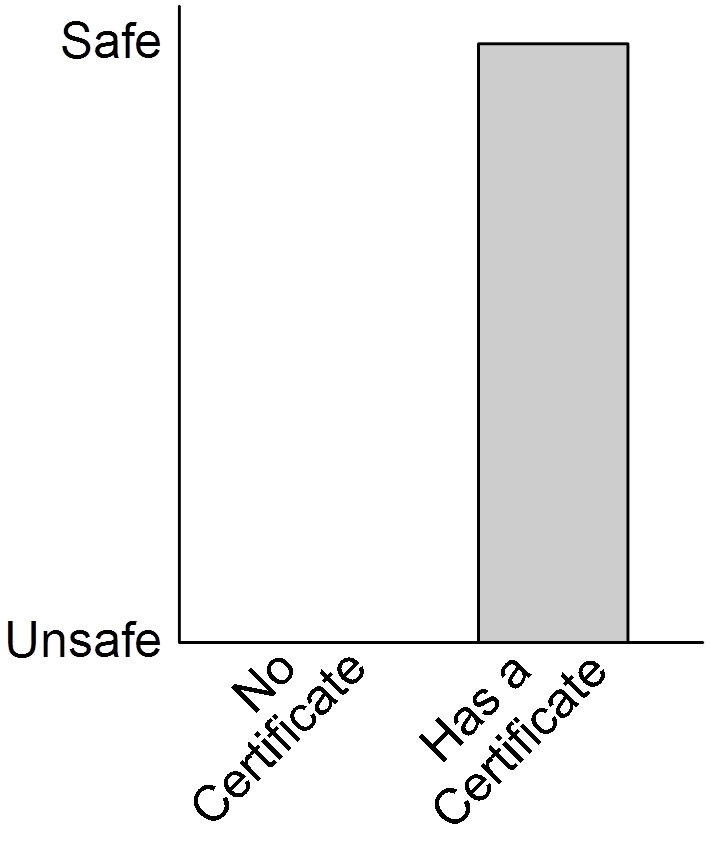
\includegraphics[width=4cm]{Hlebnikov1.png}
  \caption{SSL-безопасность в Web: что предполагалось}
  \label{Hlebnikov1}
\end{figure}

\end{center}

Однако, реальность оказалась сложнее. Например, пользоваться SSL стали
и компьютерные преступники.

Cкриншот с форума, где DDOS-еры предлагают свои услуги: 

\begin{center}

\begin{figure}[!h]
  \centering
  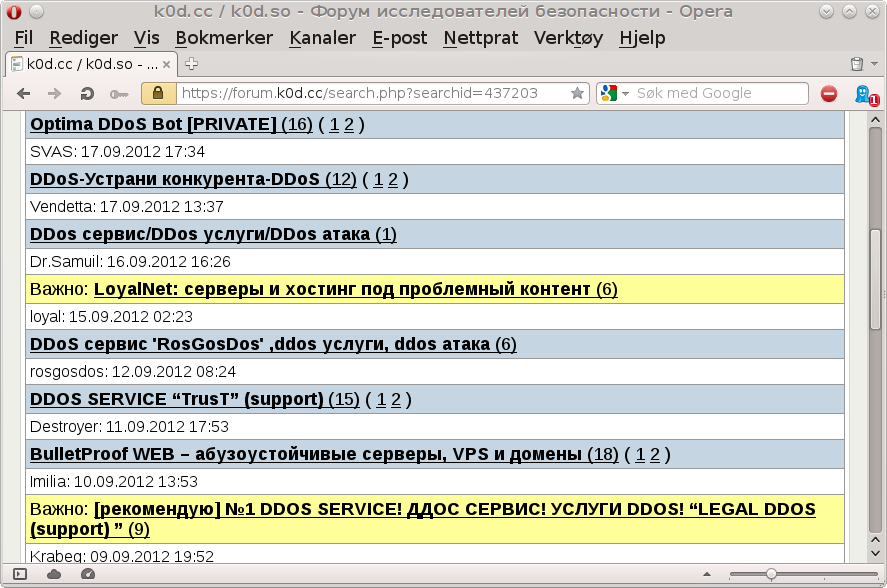
\includegraphics[width=10cm]{Hlebnikov2.png}
 \caption{Форум киберпреступников, на котором предлагаются услуги DDOS. SSL-сертификат успешно прошёл проверку}

  \label{Hlebnikov2}
\end{figure}

\end{center}

Как видно, SSL-сертификат успешно проверен, замочек показан.
Пользователь может быть уверен, с сайтом <<всё в порядке>>.

%А вот скриншот с сайта visa.com:

\begin{center}
\begin{figure}[!h]
  \centering
  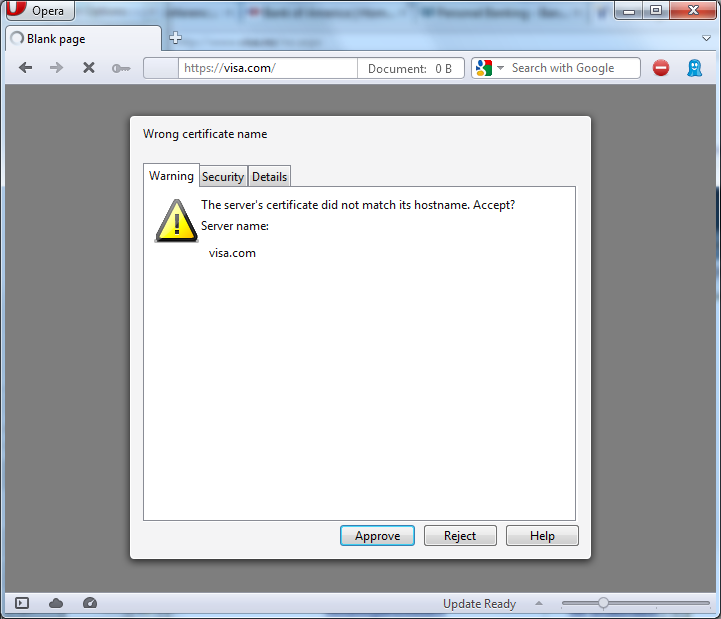
\includegraphics[width=10cm]{Hlebnikov3.png}
  \caption{Сайт платёжной системы Visa. SSL-сертификат не прошёл проверку}
  \label{Hlebnikov3}
\end{figure}
\end{center}

Видим, что сертификат браузеру определённо не нравится ~\ref{Hlebnikov3}. Внимательный
читатель наверное уже догадался, что сертификат выписан на имя
<<www.visa.com>>, а введённый адрес ~--- просто <<visa.com>>, без префикса
<<www>>. Но обычный пользователь вряд ли это поймёт, а вполне может
подумать, что его атакуют.

Совсем плохо приходится некоммерческим CA. Их сертификаты будут
признаны недействительными без ручной установки в браузер, а значит
у большинства пользователей. Браузер отвергает даже сам сайт такого
CA ~\ref{Hlebnikov4}:

\begin{center}
\begin{figure}[h!]
  \centering
  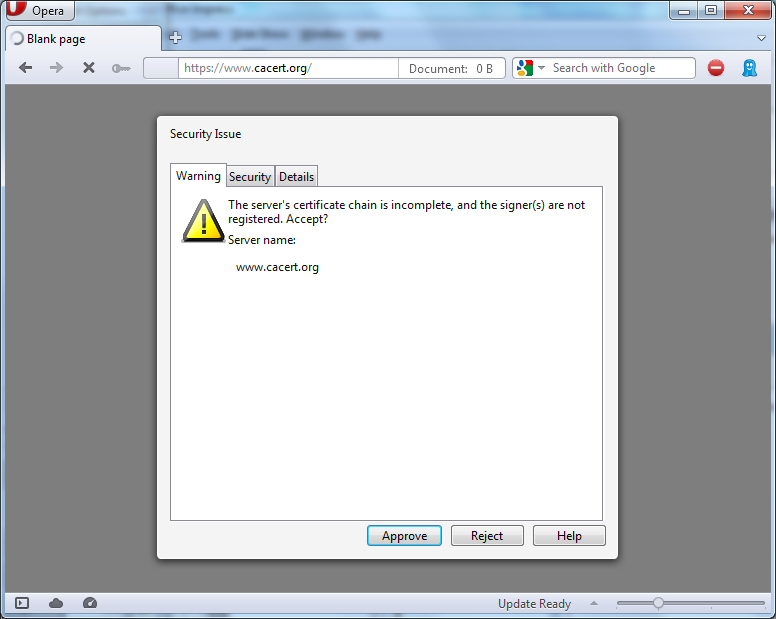
\includegraphics[width=10cm]{Hlebnikov4.png}
  \caption{Сайт некоммерчесского CA. SSL-сертификат не прошёл проверку}
  \label{Hlebnikov4}
\end{figure}
\end{center}
Заметим, что браузеры совсем не выдают таких предупреждений для
сайтов, которые предоставляются не по HTTPS, а по HTTP, то есть
вообще без сертификата. Таким образом, упрощённая модель
SSL-безопасности в Web выглядит скорее ~\ref{Hlebnikov5}, что не очень логично, так как <<плохой>> сертификат всё-таки лучше его
отсутствия.

\begin{center}
\begin{figure}[h!]
  \centering
  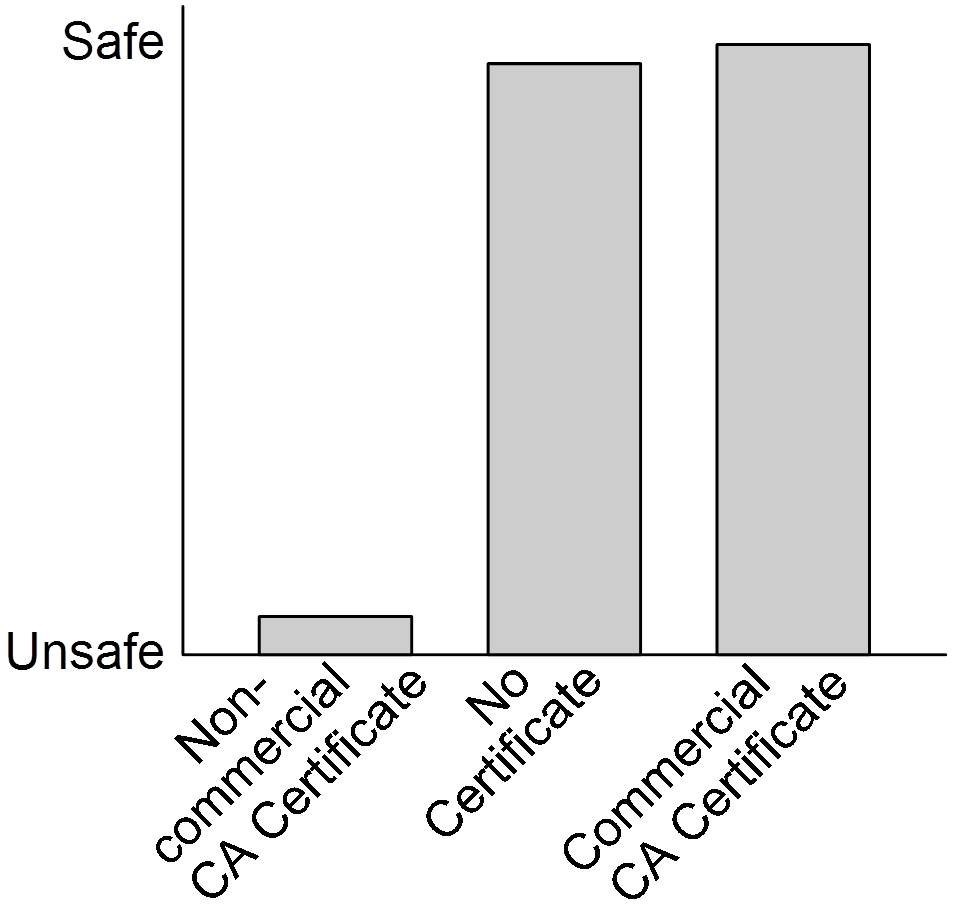
\includegraphics[width=6cm]{Hlebnikov5.png}
  \caption{SSL-безопасность в Web: что получилось}
  \label{Hlebnikov5}
\end{figure}
\end{center}

Логичнее было бы ~\ref{Hlebnikov6}.
\begin{center}
\begin{figure}[h!]
  \centering
  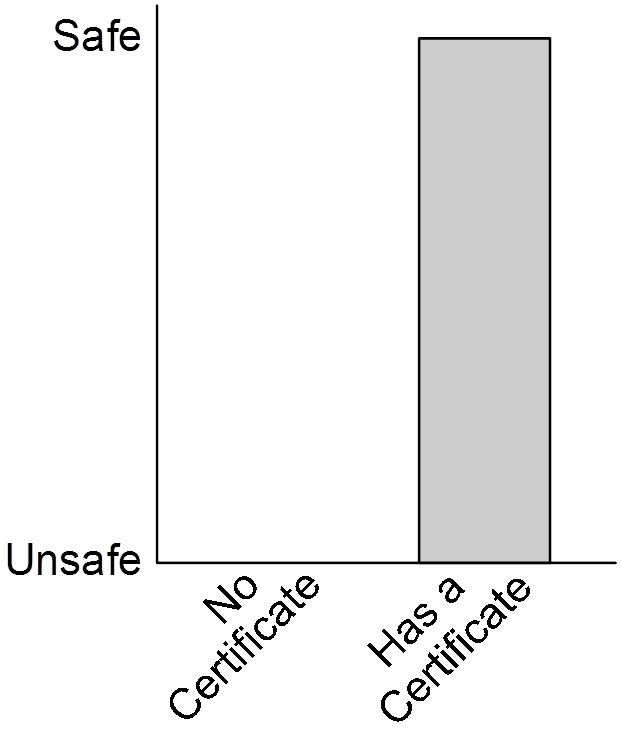
\includegraphics[width=6cm]{Hlebnikov6.png}
  \caption{SSL-безопасность в Web: что было бы логичнее}
  \label{Hlebnikov6}
\end{figure}
\end{center}
\subsection*{Взломы SSL}

На этом проблемы SSL не заканчиваются. За прошедшие годы случались
инциденты и взломы CA-инфраструктуры. Вот их неполный список:

\begin{itemize}
  \item 2001 ~--- Атакующий прикинулся сотрудником Microsoft и получил у
  Verisign сертификат для Microsoft.
  \item 2008 ~--- На сервисе live.com зарегистрирован бесплатный e-mail
  sslcertificates@live.com, затем у Thawte получен сертификат для
  login.live.com.
  \item 2008 ~--- Взломы StartCom и Comodo, у Comodo получен сертификат для
  www.mozilla.com.
  \item 2009 ~--- Взлом ipsCA через NULL prefix attack, получен сертификат для
  www.paypal.com.
  \item 2011 ~--- Взломы Comodo, Diginotar и TurkTrust. Получены сертификаты
  для \url{www.google.com}, \url{mail.google.com}, \linebreak \url{addons.mozilla.org},
  \url{login.live.com}, \url{login.yahoo.com}, \linebreak \url{login.skype.com}. Шуточная атака
  <<Honest Achmed>> на Mozilla.
  \item 2014 ~--- Взлом NICCA, получены сертификаты для доменов Google и Yahoo.
  \item 2015 ~--- Взломы CNNIC, WoSign, Let's Encrypt и Symantec. Получены
  сертификаты для доменов Google, GitHub и других.
  \item 2016 ~--- Найдены уязвимости в инфрастркутурах выдачи сертификатов у
  StartCom и Comodo. Были ли эти уязвимости использованы и как ~--- пока
  неизвестно.
\end{itemize}

А также взломы разной степени эффективности самого протокола SSL/TLS:

\begin{itemize}
  \item 2009 ~--- Renegotiation attack, SSL stripping.
  \item 2011 ~--- BEAST, StartTLS injection.
  \item 2012 ~--- CRIME.
  \item 2013 ~--- BREACH, TIME, Lucky13.
  \item 2014 ~--- FREAK, POODLE, Triple Handshake.
  \item 2016 ~--- DROWN.
\end{itemize}

А также не будем забывать о периодически находимых уязвимостях в
реализациях SSL, например Heartbleed в OpenSSL.

\subsection*{Система CA недостаточно надёжна}

До сих пор никто так и смог дать убедительного ответа, почему сайты и
пользователи должны доверять тем самым CA, которых большинство
пользователей в глаза не видело. Ответ <<по умолчанию>> на этот вопрос -
потому что CA берут деньги за выдачу сертификата, и если они вдруг
выдадут неправильный сертификат или будут взломаны ~--- сразу потеряют
доверие, клиентов и разорятся. Мне в этот аргумент почему-то не
очень-то верится. Особенно в свете известных вышеперечисленных
взломов. Кто из CA понёс серьёзное наказание в результате взлома и
прекратил выдачу сертификатов? Почти никто. Только маленький
Diginotar. А взлом Comodo в том же году, наделавший немало шума -
спустили на тормозах. Потому что Comodo ~--- <<too big to fail>>. Работает
дальше и продолжает <<радовать>> нас периодическими уязвимости своей
инфраструктуры выдачи сертификатов. А сколько взломов не стало
достоянием общественности? А ведь CA довольно неохотно раскрывают
факты взломов своей инфраструктуры, и бывали уличены в сокрытии такой
информации.

А можем ли мы быть уверены, что если в офис CA придут
сотрудники местных спецслужб и попросят выдать им сертификат на не
принадлежащий им домен, то СА откажет им? Скорее, мы можем быть
уверены в обратном. А знает ли уважаемый читатель, что в США полицией
и спецслужбами уже несколько лет используются так называемые MITM
boxes? Это устройство, которое в реальном времени осуществляет
MITM-атаку и расшифровывает весь SSL-траффик, проходящий через
устройство. Причём, пользователь, которого прослушивают, не получает
никаких предупреждений от своего браузера, потому что MITM-box на лету
выдаёт <<правильные>> сертификаты для всех серверов, посещаемых
пользователем. Как устройчтво это делает? Очень просто ~--- устройство
обладает intermediate-CA сертификатом, который любезно выдан крупным
американским CA, которому, конечно, доверяют все браузеры.

Большая проблема здесь ~--- то что абсолютно любой CA может выдать
сертификат абсолютно любому сайту. Это ещё хуже, чем единая точка
отказа. Доверие CA-центрам ~--- абсолютно, а они его, прямо скажем,
не заслужили.

А ещё некоторые CA доверяют выдачу своих сертификатов другим фирмам,
эдаким дилерам. Прямо как подключение телефона в салоне связи. А ещё
многие CA вполне официально выдают некоторым крупным бизнес-клиентам
сертификаты, позволяющие выдавать другие сертификаты, то есть частично
делегируют полномочия CA. Всё это увеличивает прибыль CA, но,
к сожалению, уменьшает безопасность сайтов и пользователей.

\subsection*{Чем отвечает индустрия}

Как видно, в проблем в концепции SSL и CA хватает. Чем же отвечает
индустрия? Правильно, индустрия отвечает закручиванием гаек. <<PKI them
harder>>. В частности, предлагались или предлагаются следующие решения:

\begin{itemize}
  \item Короткоживущие сертификаты
  \item Публичные списки выдаваемых сертификатов
  \item Обязательное OCSP
  \item HTTP Strict Transport Security (HSTS)
  \item HTTP Public Key Pinning (HPKP) и TACK
  \item Convergence и Mutually Endorsing CA Infrastructure
  \item The Monkeysphere Project и Web of Trust
\end{itemize}

Некоторые из этих предложений хороши, некоторые сомнительны, некоторые
уже не выдержали испытание временем, но большинство из них пытаются
<<наложить заплатки>> на существующую систему SSL и CA, вместо того,
чтобы взглянуть на проблему шире. Ведь наша цель ~--- повысить безопасность
пользователя, и закручивание гаек в PKI ~--- далеко не единственный
способ.

\subsection*{Диверсификация защиты  и управление рисками}

PKI ~--- не серебрянная пуля. И не священная корова. Нужна диверсификация
средств безопасности. Не стоит складывать все яйца в одну корзину,
полагаясь лишь на PKI.

Диверсификация защиты применяется в реальном мире с начала времён. Её
преимущество очевидны ~--- нет единой точки отказа. Если механизм защиты
вдруг отказал, то

\begin{itemize}
  \item без диверсификации ~--- отказала вся система,
  \item с диверсификацией ~--- возрос риск, но не отказала вся система.
\end{itemize}

Безопасность с помощью диверсифицированной защиты и управления рисками:

\begin{itemize}
  \item Применяется комплекс защитных мер.
  \item Ни одна из мер сама по себе не даёт сильной защиты.
  \item Комбинация защитных мер даёт сильную защиту.
  \item Возможна детальная оценка безопасности и <<обратная связь>>.
\end{itemize}

\subsection*{Оценка уровня безопасности сайта}

Браузер должен оценивать уровень безопасности сайта исходя из многих
критериев, чтобы предоставлять комплексную диверсифицированную
защиту. Что же можно использовать в качестве таких критериев?

Прежде всего, несколько предложений относительно самого SSL.

Так повелось, что SSL применяют как абсолютно <<беcпамятную>>
технологию. В отличие от, например, SSH. Каждое общение с сайтом ~--- как
в первый раз. Сменился сертификат у сервера ~--- никакой реакции у
браузера на это. Сменился CA ~--- тоже никакой реакции.

Следующие факторы должны понижать оценку безопасности сайта:

\begin{itemize}
  \item У сайта другой сертификат\begin{itemize}
  \item И срок действия предыдущего не вышел
\end{itemize}


  \item У сертификата другой ключ\begin{itemize}
  \item И предыдущий сертификат не отозван
\end{itemize}


  \item Внезапная смена CA\begin{itemize}
  \item Французский CA, бразильский сайт?
\end{itemize}


  \item Смена EV на DV
\end{itemize}

<<Память>> неплохо бы использовать не только для SSL, но и для IP:

\begin{itemize}
  \item Кардинально сменился IP\begin{itemize}
  \item Совсем другая подсеть?
  \item Совсем другая страна?
\end{itemize}


  \item Traceroute стал гораздо короче (MITM?)
\end{itemize}

Браузер должен помнить о ранее посещённых сайтах, когда сайт просит
пароль:

\begin{itemize}
  \item Сайт посещался много раз, и много раз пароль здесь уже вводился -
  риск меньше.
  \item Сайт посещается в первый раз и уже просит пароль ~--- риск больше.
\end{itemize}

Хостинг. Стоит проверить whois и AS (autonomous system) info.

Пример: банк Societe Generale.

\begin{itemize}
  \item Хостится на AS.
  \item Имя AS: SOCIETE-GENERALE.
  \item Подключена к французскому бэкбону.
  \item Работает с 1995 года.
\end{itemize}

Такой хостинг заслуживает доверия.

По части DNS можно проверить следующее:

\begin{itemize}
  \item Reverse lookup: \url{client321.adsl-pool.isp.com}
  \item Маленький TTL
  \item Комбинация записей A, MX, NS
  \item Регистратор DNS и IP:\begin{itemize}
  \item RIPE: риск меньше
  \item GoDaddy: риск больше
\end{itemize}


\end{itemize}

Можно проверить и TCP/IP stack fingerprint сервера:

\begin{itemize}
  \item E-commerce сайт хостится на Windows Home Premium?
  \item Открыт порт, по которому слушает <<популярный>> троян?
\end{itemize}

Проверка URL:

\begin{itemize}
  \item Смешанный алфавит в именах популярных сайтов.
  \item Spell-check: \url{panascanic.com}, \url{bankoffireland.ie}.
  \item Подстроки: <<members>>, <<adsl-pool>>, etc.
\end{itemize}

Мы видим ту же веб-страницу, что и остальные Интернет-\linebreak пользователи,
или нам её подменили?

\begin{itemize}
  \item Сравнение с веб-архивом.
  \item Сравнение с кэшем Google.
  \item Сравнение с User Agent = Googlebot.
\end{itemize}

Проверка содержания самой веб-страницы:

\begin{itemize}
  \item Страница пытается задействовать известные уязвимости?
  \item HTML тэги в <<неправильных>> местах?
  \item Несколько тэгов html, head, title, body?
  \item Много объектов подгружается из других доменов?
\end{itemize}

Проверка Javascript на странице:

\begin{itemize}
  \item Длинные строки и их энтропия.
  \item Вызовы eval(), большое количество substring(), concat(), \linebreak fromCharCode().
\end{itemize}

Для оценки безопасности страницы наверняка можно использовать и
байесовский фильтр, широко применяемый для оценки безопасности e-mail
и борьбы со спамом.

Злоумышленники могут препятствовать анализу страницы с помощью
обфускации, но обфускация сама по себе вызывает подозрение, а значит
снижает оценку безопасности.

После всех проверок, оценка безопасности сайта может выглядеть,
например, ~\ref{Hlebnikov7}.

\begin{center}
\begin{figure}[h!]
  \centering
  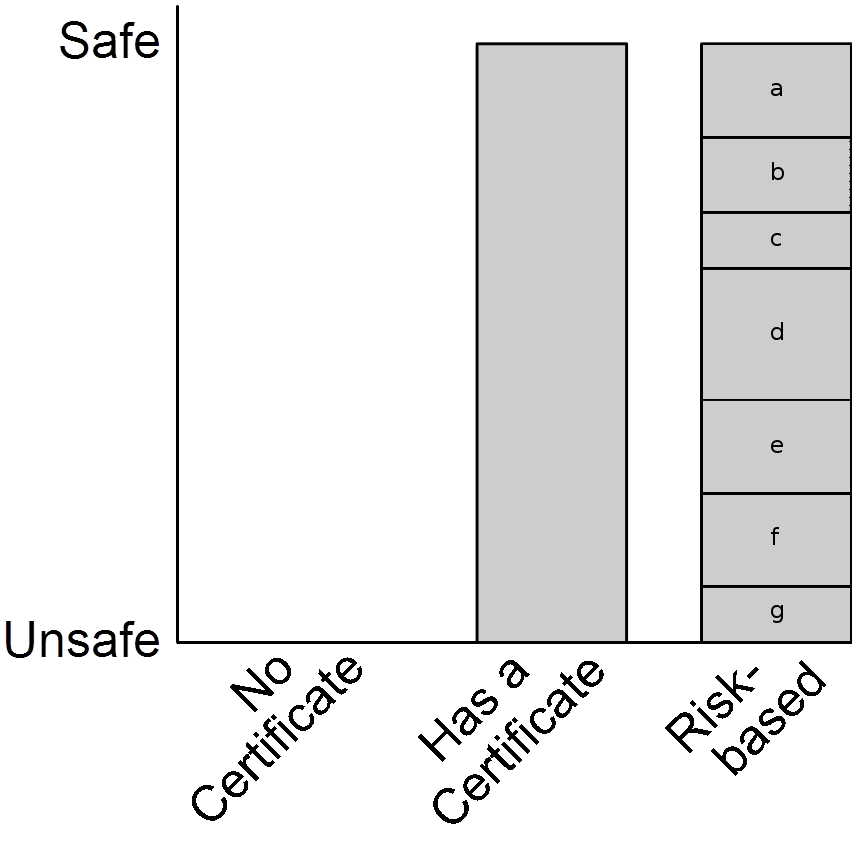
\includegraphics[width=8cm]{Hlebnikov7.png}
  \caption{Пример оценки безопасности Web-сайта при использовании управления рисками}
  \label{Hlebnikov7}
\end{figure}
\end{center}

\end{document}

\documentclass[10pt, a5paper]{article}
\usepackage{pdfpages}
\usepackage{parallel}
\usepackage[T2A]{fontenc}
\usepackage{ucs}
\usepackage[utf8x]{inputenc}
\usepackage[polish,english,russian]{babel}
\usepackage{hyperref}
\usepackage{rotating}
\usepackage[inner=2cm,top=1.8cm,outer=2cm,bottom=2.3cm,nohead]{geometry}
\usepackage{listings}
\usepackage{graphicx}
\usepackage{wrapfig}
\usepackage{longtable}
\usepackage{indentfirst}
\usepackage{array}
\newcolumntype{P}[1]{>{\raggedright\arraybackslash}p{#1}}
\frenchspacing
\usepackage{fixltx2e} %text sub- and superscripts
\usepackage{icomma} % коскі ў матэматычным рэжыме
\PreloadUnicodePage{4}

\newcommand{\longpage}{\enlargethispage{\baselineskip}}
\newcommand{\shortpage}{\enlargethispage{-\baselineskip}}

\def\switchlang#1{\expandafter\csname switchlang#1\endcsname}
\def\switchlangbe{
\let\saverefname=\refname%
\def\refname{Літаратура}%
\def\figurename{Іл.}%
}
\def\switchlangen{
\let\saverefname=\refname%
\def\refname{References}%
\def\figurename{Fig.}%
}
\def\switchlangru{
\let\saverefname=\refname%
\let\savefigurename=\figurename%
\def\refname{Литература}%
\def\figurename{Рис.}%
}

\hyphenation{admi-ni-stra-tive}
\hyphenation{ex-pe-ri-ence}
\hyphenation{fle-xi-bi-li-ty}
\hyphenation{Py-thon}
\hyphenation{ma-the-ma-ti-cal}
\hyphenation{re-ported}
\hyphenation{imp-le-menta-tions}
\hyphenation{pro-vides}
\hyphenation{en-gi-neering}
\hyphenation{com-pa-ti-bi-li-ty}
\hyphenation{im-pos-sible}
\hyphenation{desk-top}
\hyphenation{elec-tro-nic}
\hyphenation{com-pa-ny}
\hyphenation{de-ve-lop-ment}
\hyphenation{de-ve-loping}
\hyphenation{de-ve-lop}
\hyphenation{da-ta-ba-se}
\hyphenation{plat-forms}
\hyphenation{or-ga-ni-za-tion}
\hyphenation{pro-gramming}
\hyphenation{in-stru-ments}
\hyphenation{Li-nux}
\hyphenation{sour-ce}
\hyphenation{en-vi-ron-ment}
\hyphenation{Te-le-pathy}
\hyphenation{Li-nux-ov-ka}
\hyphenation{Open-BSD}
\hyphenation{Free-BSD}
\hyphenation{men-ti-on-ed}
\hyphenation{app-li-ca-tion}

\def\progref!#1!{\texttt{#1}}
\renewcommand{\arraystretch}{2} %Іначай формулы ў матрыцы зліпаюцца з лініямі
\usepackage{array}

\def\interview #1 (#2), #3, #4, #5\par{

\section[#1, #3, #4]{#1 -- #3, #4}
\def\qname{LVEE}
\def\aname{#1}
\def\q ##1\par{{\noindent \bf \qname: ##1 }\par}
\def\a{{\noindent \bf \aname: } \def\qname{L}\def\aname{#2}}
}

\def\interview* #1 (#2), #3, #4, #5\par{

\section*{#1\\{\small\rm #3, #4. #5}}

\def\qname{LVEE}
\def\aname{#1}
\def\q ##1\par{{\noindent \bf \qname: ##1 }\par}
\def\a{{\noindent \bf \aname: } \def\qname{L}\def\aname{#2}}
}

\switchlang{ru}
\begin{document}
\title{Превращение Android-устройств в мобильные серверы при помощи FOSS\footnote{\url{vitalyok@tut.by} \url{http://lvee.org/ru/abstracts/252}}}
\author{Виталий Сороко, Minsk, Belarus}
\maketitle
\begin{abstract}
Modern mobile devices such as smartphones and tablets now have powerful processors and sometime large amount of memory inside.  So these devices can be suitable for standard server tasks, for example data warehousing and HTTP request handling. However, since the architecture of mobiles is different from standard PCs and servers, it is necessary to recompile open source server software  for further usage. This is not very simple process and here is the description of key points and main ways of that.
\end{abstract}
Современные мобильные устройства, такие как смартфоны, планшеты и даже «умные» часы, с каждым годом становятся всё мощнее и мощнее. Благодаря увеличивающемуся объему памяти, многоядерным процессорам и наличию встроенной батареи они вполне могут работать в качестве маленького переносного сервера, ведь у них внутри есть все что для этого нужно – вычислительные мощности и резервный источник питания на случай сбоя в энергосети. Однако, процесс превращения мобильного устройства в маленький переносной сервер не так прост как может показаться на первый взгляд.  Для того чтобы сделать это, вам придётся пройти через следующие основные шаги:

\begin{enumerate}
  \item Покупка и подготовка оборудования.
  \item Выбор набора необходимого серверного ПО
  \item Компиляция, установка и настройка серверного ПО
  \item Проверка работоспособности системы
  \item Оптимизация
\end{enumerate}

Итак первым этапом является покупка и подготовка оборудования. Как известно, для работы серверного ПО вам понадобиться сам сервер и сетевое соединения, а также оборудование для обеспечения работы сетевого соединения. В качестве сервера мы будем использовать мобильное устройство. Поэтому, вам понадобиться смартфон, планшет или какой либо другой гаджет на базе Android. Кроме этого, необходимо также определиться будет ли вам достаточно только соединения по WiFi или 3G/4G/LTE. Для того чтобы это сделать, нужно чётко понимать в каких целях будет использоваться ваш сервер. Если это будет простой веб-сервер, предназначенный для выполнения задач, которым не требуется постоянное, надёжное и безопасное соединение, то  вполне будет достаточно 3G/4G/LTE соединения со статическим IP-адресом или обмена данными через WiFi-маршрутизатор. Совсем другое дело если вы захотите сделать максимально приближённый аналог обычного сервера, работающий по проводному соединению. Для этого вам понадобится либо устройство изначально оборудованное Ethernet-портом (а таких сейчас продаётся не очень много), либо переходник OTG и USB-сетевой адаптер (перед покупкой вам необходимо проверить поддерживает ли ваше устройство работу в качестве USB-хоста при подключении данного переходника). Кроме этого, в случае OTG-переходника и внешней USB сетевой карты вам необходимо будет также настроить проводную сеть, а это в зависимости от устройства может представлять собой не очень простой процесс.

На втором этапе вам необходимо определиться с серверным программным обеспечением, то есть выбрать подходящий веб-сервер, СУБД, а также другие вспомогательные компоненты. После этого, вам нужно будет загрузить их на ваше устройство. Тут к слову, как и в обычных Linux системах  способы могут быть разные. Самый легкий способ это конечно поиск и установка готового набора через Google Play. Главный недостаток данного способа – это зависимость от поставщика набора серверных компонентов, а именно вы будет пользоваться серверными компонентами только тех версий, которые доступны  в данном наборе, а обновления будут приходит только вместе с обновлением Android приложения, содержащего данный набор. К слову, из личного опыта, могу с уверенностью сказать что многие приложения содержащие такие наборы очень часто не обновляются. Кроме этого, за Android приложения содержащие внутри себя набор серверных компонентов вам скорее всего придётся заплатить тем или иным образом (либо путём покупки приложения, либо путём просмотра содержащейся в нём рекламы). Поэтому, этим способом я рекомендую пользоваться только если вы совсем не понимаете что такое Linux и как на нём можно устанавливать приложения из исходных кодов. Кроме первого способа на просторах интернета вы можете найти статьи про то, что установить серверные компоненты на Android вам поможет приложение BotBrew (или аналогичное). В целом могу сказать, что данный способ вполне работоспособен, но есть несколько «но». Во первых эта  BotBrew совместим далеко не со всеми устройствами. Во вторых он сильно грузит мобильное устройство. И в третьих эта штука по сути представляет собой что-то среднее, а именно после её установки вы получите некое подобие Debian репозитория из которого можно устанавливать приложения  таким же способом как и в Debian. С одной стороны это хорошо, а с другой проблемы не самых свежих версий серверных компонентов никуда не исчезнут. В общем это способ могу рекомендовать только в тех случаях когда вам лень возиться с компиляцией из исходных кодов, вы хорошо знаете что такое Debian и на сто процентов уверены что на вашем устройстве это будет работать,  а также если снижение производительности устройства вас не сильно беспокоит. И на всякий случай поделюсь своим опытом использования данной программы: после её установки планшет на базе Android 4 стал медленно работать и регулярно делать оптимизацию установленных приложений. После того как я понял в чём дело, удалить BotBrew позволил только сброс устройства на заводские настройки (Hard reset). Итого, если после прочитанного вы поняли что первых два способа вам не подойдут, то скорее всего мне удалось вас убедить что наиболее правильный и хороший способ установки серверных компонентов – это их сборка, компиляция и установка из исходных кодов. Ведь только так вы получите у себя на устройстве самые свежие версии  компонентов, которые к тому же будут относительно быстро работать и безо всякой рекламы.

Итак, теперь чуть больше конкретики про процесс сборки, компиляции и установки приложений из исходных кодов под Android. В целом он полностью аналогичен таковому в обычном линуксе. Вам нужно будет скачать исходные коды с официальных сайтов (репозиториев) выбранных компонентов и приступить к компиляции и установке. Для этого , как и в Linux, вам надо будет использовать команду ./configure  и make. Тем не менее есть и отличия. Так, например, в общем случае вам необходимо будет скачать и установить на ваш компьютер Eclipse с CDT, Android SDK, NDK и прочие необходимые компоненты и библиотеки. Сама сборка и компиляция для Android устройства будет осуществляться на вашем персональном компьютере. Далее после сборки и компиляции вам необходимо будет поместить полученный результат на Android устройство и немного «поколдовать» для его настройки и запуска. Для этого нужно будет проверить сетевые настройки, конфигурационные файла каждого из серверных компонентов, ну и конечно проверить работает всё это или нет при помощи браузера (в случае веб сервера) или клиента (в случае СУБД и других сервисов). По сути это и есть этап проверки работоспособности. После завершения данного этапа можно будет смело попробовать сделать своё собственное приложение с набором серверных компонентов, но это не очень простой процесс, который имеет свои особенности и поэтому выходит за рамки данной темы, так как заслуживает отдельного рассмотрения.

Ну и в завершении, хочу сказать пару слов про оптимизацию. Если честно то без неё можно обойтись, но всё-таки лучше этим заняться. На мой взгляд оптимизировать надо всё, но в меру. Начинать оптимизацию я рекомендую с измерения производительности выбранных вами серверных компонентов и их влияния на систему в целом. Сейчас существует огромное множество различных программ-мониторов на любой вкус и цвет, поэтому мне даже сложно порекомендовать что-то конкретное. Ваша главная задача – это проверить при помощи таких программ не появилось ли у вас на мобильном устройстве какого либо серверного компонента который перегружает ваше устройство. Если случилось именно так, то вам необходимо либо произвести оптимизацию серверного компонента за счёт изменения настроек в конфигурационном файле или файлах данного компонента, либо, если первое не помогло, самое время задуматься о выборе другого компонента выполняющего данные функции. Как известно в мире Opensource обычно существует немалое число различных веб-сереверов, СУБД и прочих серверных приложений с отрытыми исходными кодами и вы всегда можете выбрать какую либо более легковесную замену с аналогичным функционалом. Кроме такого рода оптимизаций, в некоторых случаях могут быть также полезны архитектурные и аппаратные оптимизации. Например если мобильное устройство не тянет нужный вам набор серверных компонентов, то можно либо купить более мощное устройство взамен прежнего, либо разнести серверные компоненты на несколько устройств, тем самым поменяв архитектуру.

И последнее: в качестве подведения итогов я решил написать пару слов про то, зачем это всё нужно и почему вообще я решил этим заняться. Превращение мобильного устройства в сервер даёт целый ряд преимуществ: меньшее энергопотребление по сравнению со стандартными серверами, высокая мобильность (вы можете всегда взять сервер с собой куда угодно), ну и конечно мобильные устройства занимают гораздо меньше физического пространства чем, например, их братья в модульном исполнении (серверы типоразмера 1U). У мобильных устройств, превращенных в серверы, есть конечно и недостатки, один из которых производительность, но тут всё зависит от того что и с чем сравнивать.

\end{document}

\documentclass[10pt, a5paper]{article}
\usepackage{pdfpages}
\usepackage{parallel}
\usepackage[T2A]{fontenc}
\usepackage{ucs}
\usepackage[utf8x]{inputenc}
\usepackage[polish,english,russian]{babel}
\usepackage{hyperref}
\usepackage{rotating}
\usepackage[inner=2cm,top=1.8cm,outer=2cm,bottom=2.3cm,nohead]{geometry}
\usepackage{listings}
\usepackage{graphicx}
\usepackage{wrapfig}
\usepackage{longtable}
\usepackage{indentfirst}
\usepackage{array}
\newcolumntype{P}[1]{>{\raggedright\arraybackslash}p{#1}}
\frenchspacing
\usepackage{fixltx2e} %text sub- and superscripts
\usepackage{icomma} % коскі ў матэматычным рэжыме
\PreloadUnicodePage{4}

\newcommand{\longpage}{\enlargethispage{\baselineskip}}
\newcommand{\shortpage}{\enlargethispage{-\baselineskip}}

\def\switchlang#1{\expandafter\csname switchlang#1\endcsname}
\def\switchlangbe{
\let\saverefname=\refname%
\def\refname{Літаратура}%
\def\figurename{Іл.}%
}
\def\switchlangen{
\let\saverefname=\refname%
\def\refname{References}%
\def\figurename{Fig.}%
}
\def\switchlangru{
\let\saverefname=\refname%
\let\savefigurename=\figurename%
\def\refname{Литература}%
\def\figurename{Рис.}%
}

\hyphenation{admi-ni-stra-tive}
\hyphenation{ex-pe-ri-ence}
\hyphenation{fle-xi-bi-li-ty}
\hyphenation{Py-thon}
\hyphenation{ma-the-ma-ti-cal}
\hyphenation{re-ported}
\hyphenation{imp-le-menta-tions}
\hyphenation{pro-vides}
\hyphenation{en-gi-neering}
\hyphenation{com-pa-ti-bi-li-ty}
\hyphenation{im-pos-sible}
\hyphenation{desk-top}
\hyphenation{elec-tro-nic}
\hyphenation{com-pa-ny}
\hyphenation{de-ve-lop-ment}
\hyphenation{de-ve-loping}
\hyphenation{de-ve-lop}
\hyphenation{da-ta-ba-se}
\hyphenation{plat-forms}
\hyphenation{or-ga-ni-za-tion}
\hyphenation{pro-gramming}
\hyphenation{in-stru-ments}
\hyphenation{Li-nux}
\hyphenation{sour-ce}
\hyphenation{en-vi-ron-ment}
\hyphenation{Te-le-pathy}
\hyphenation{Li-nux-ov-ka}
\hyphenation{Open-BSD}
\hyphenation{Free-BSD}
\hyphenation{men-ti-on-ed}
\hyphenation{app-li-ca-tion}

\def\progref!#1!{\texttt{#1}}
\renewcommand{\arraystretch}{2} %Іначай формулы ў матрыцы зліпаюцца з лініямі
\usepackage{array}

\def\interview #1 (#2), #3, #4, #5\par{

\section[#1, #3, #4]{#1 -- #3, #4}
\def\qname{LVEE}
\def\aname{#1}
\def\q ##1\par{{\noindent \bf \qname: ##1 }\par}
\def\a{{\noindent \bf \aname: } \def\qname{L}\def\aname{#2}}
}

\def\interview* #1 (#2), #3, #4, #5\par{

\section*{#1\\{\small\rm #3, #4. #5}}

\def\qname{LVEE}
\def\aname{#1}
\def\q ##1\par{{\noindent \bf \qname: ##1 }\par}
\def\a{{\noindent \bf \aname: } \def\qname{L}\def\aname{#2}}
}

\switchlang{ru}
\begin{document}
\title{Практическое использование сервисов контейнеризации в облаке Амазон}
\author{Andrew Rewoonenco, Minsk, Belarus\footnote{\url{arewoonenco@gmail.com} \url{https://lvee.org/ru/abstracts/255}}}
\maketitle
\begin{abstract}
Amazon cloud service (AWS) provides several container-based services (EC2 CS, Lambda, CodeBuild). These services are quite special to Amazon and differ a lot from Open Source analogs however based on them. The goal of this report is to review common problems based on real experience and to show solutions author had find out.
\end{abstract}

\subsection*{Введение}
Современные технологии часто ориентируются на облачные сервисы из-за их
высокой надёжности и простой расширяемости. Один из старейших облачных
провайдеров это Амазон (обычно сокоащаемый до AWS). Он предоставляет
огромный набор различных сервисов, очень хорошо связанных в единое целое.

Здесь мы затронем сервисы, связаные с контейнеризацией.
Доклад основан исключительно на эмпирических выводах (реальном
использовании), и иногда достаточно сильно расходится с декларируемыми или
ожидаемыми особенностями сервисов и их использования.

Из большого набора сервисов Амазона с контейнеризацией мы рассмотрим
несколько сервисов, по которым есть достаточно достоверная выборка:

\begin{itemize}
\item сервис контейнеризации Амазона (EC2 CS);
\item сервис краткосрочных операций (Lambda);
\item сервис компиляции/тестирования (CodeBuild).
\end{itemize}

Общее у них следующее:

\begin{enumerate}
\item Все эти сервисы запускаются на виртуальных машинах (инстансах), работающих под управлением Amazon Linux.
\item Они построены на сервисе контейнеризации docker.
\item Возможно контролировать практически все параметры контейнера.
\end{enumerate}

Рассмотрим декларируемое назначение, недостатки и способы их исправления
для каждого из сервисов.

\subsection*{Сервис контейнеризации Амазона (EC2 CS)}

Декларируемое назначение данного сервиса это разнообразные
высокодоступные сервисы, обслуживающие входящий трафик, преимущественно
веб-сервисы.

Обычный сценарий работы: создаётся кластер контейнеров из нескольких ВМ
(инстансов), и сервис запускается на них. Для высокодоступности
используется ещё один сервис Амазона --- Балансировщик (ELB),
перенаправляющий запросы по необходимости в несколько контейнеров и даже
умеющий расширять их число при повышении нагрузки.

Но в реальных сценариях использования он имеет ряд недостатков:

\begin{enumerate}
\item Фиксированное ограничение CPU/Memory.
\item При размещении нескольких контейнеров на 1 ВМ это не работает, если
  котнейнеры используют одни и те же порты.
\item Не умеет распределять контейнеры правильно по датацентрам Амазона
  (Availability Zone), и из-за этого нестабильно работает балансировщик
  нагрузки.
\item Псегда надо иметь резерв по ВМ, иначе при перезапуске сервиса можно
  попасть в Deadlock.
\end{enumerate}


\subsection*{Сервис краткосрочных операций (Lambda)}

Декларируемое назначение данного сервиса это разнообразные
высокодоступные краткосрочные клиент-сервисы, например, системы
мониторинга, контроля, сообщений. Имеют жёткий лимит на время действия
--- не более 5 минут, используют только скрипт для работы (python, java
jar, javascript nodejs). Не имеют входящих портов принципиально, но умеют
обрабатывать сообщения из очередей Амазона (например SNS).

Сервис очень удобен для крошечных простейших операций (например,
проверить веб-сервера и отослать СМС в случае недоступности) но при
более-менее серьёзном использовании очень ограничен. В реальных
сценариях использования имеет ряд недостатков:

\begin{enumerate}
\item Из-за времени использования многие возможности принципиально
  недоступны.
\item Нет входящих портов или протокола UDP за редкими исключениями.
\item Отладка просто чудовищно сложна из-за использования \linebreak CloudWatch для
  хранения логов.
\item Работа с бинарными приложениями страшно неудобна и сложна.
\item Доступ к сервису SSH весьма нетривиален.
\end{enumerate}

\subsection*{Сервис компиляции/тестирования (CodeBuild)}

Декларируемое назначение данного сервиса это
компиляция/сборка/тестирование разнообразного кода. В идеале позволяет
заменить комбайн типа Jenkins на контейнеризованные решения. Стандартное
использование --- исходный код забирается с хранилища S3 (веб-хранилище
Амазона), строится в контейнере, записывается снова на S3.

Сервис очень удобен для стандартный простейших операций (скомпилировать),
но для более-менее сложных проектов ограничен. В реальных сценариях
использования имеет ряд недостатков:

\begin{enumerate}
\item Для сервиса надо вначале подготовить базовый контейнер с системой
  сборки.
\item Отладка построения очень сложна из-за использования \linebreak CloudWatch для
  хранения логов.
\item Сама постройка требует очень много времени из-за частей: развернуть
  контейнер, забрать файлы, положить файлы.
\item При постройке есть фиксированный набор этапов, он выполняется весь,
  даже если этап вернул ошибку, и только в конце сообщается о неудаче.
\item Интеграция «из коробки» через CodePipeline с git (например с гитхабом)
  очень ограничена.
\end{enumerate}

\subsection*{Заключение}

Как мы видим, декларируемые и реальные сценарии использования сервисов
Амазона весьма отличаются. Несмотря на то, что все сервисы базируются
на хорошо известных открытых решениях, стандартные сценарии их
использования внутри системы Амазон не подходят. Да и рекомендованные
самим Амазоном не особо хороши при использовании, чуть отклоняющемся от стандартного.

\end{document}

%\documentclass[10pt, a5paper]{article}
\usepackage{pdfpages}
\usepackage{parallel}
\usepackage[T2A]{fontenc}
\usepackage{ucs}
\usepackage[utf8x]{inputenc}
\usepackage[polish,english,russian]{babel}
\usepackage{hyperref}
\usepackage{rotating}
\usepackage[inner=2cm,top=1.8cm,outer=2cm,bottom=2.3cm,nohead]{geometry}
\usepackage{listings}
\usepackage{graphicx}
\usepackage{wrapfig}
\usepackage{longtable}
\usepackage{indentfirst}
\usepackage{array}
\newcolumntype{P}[1]{>{\raggedright\arraybackslash}p{#1}}
\frenchspacing
\usepackage{fixltx2e} %text sub- and superscripts
\usepackage{icomma} % коскі ў матэматычным рэжыме
\PreloadUnicodePage{4}

\newcommand{\longpage}{\enlargethispage{\baselineskip}}
\newcommand{\shortpage}{\enlargethispage{-\baselineskip}}

\def\switchlang#1{\expandafter\csname switchlang#1\endcsname}
\def\switchlangbe{
\let\saverefname=\refname%
\def\refname{Літаратура}%
\def\figurename{Іл.}%
}
\def\switchlangen{
\let\saverefname=\refname%
\def\refname{References}%
\def\figurename{Fig.}%
}
\def\switchlangru{
\let\saverefname=\refname%
\let\savefigurename=\figurename%
\def\refname{Литература}%
\def\figurename{Рис.}%
}

\hyphenation{admi-ni-stra-tive}
\hyphenation{ex-pe-ri-ence}
\hyphenation{fle-xi-bi-li-ty}
\hyphenation{Py-thon}
\hyphenation{ma-the-ma-ti-cal}
\hyphenation{re-ported}
\hyphenation{imp-le-menta-tions}
\hyphenation{pro-vides}
\hyphenation{en-gi-neering}
\hyphenation{com-pa-ti-bi-li-ty}
\hyphenation{im-pos-sible}
\hyphenation{desk-top}
\hyphenation{elec-tro-nic}
\hyphenation{com-pa-ny}
\hyphenation{de-ve-lop-ment}
\hyphenation{de-ve-loping}
\hyphenation{de-ve-lop}
\hyphenation{da-ta-ba-se}
\hyphenation{plat-forms}
\hyphenation{or-ga-ni-za-tion}
\hyphenation{pro-gramming}
\hyphenation{in-stru-ments}
\hyphenation{Li-nux}
\hyphenation{sour-ce}
\hyphenation{en-vi-ron-ment}
\hyphenation{Te-le-pathy}
\hyphenation{Li-nux-ov-ka}
\hyphenation{Open-BSD}
\hyphenation{Free-BSD}
\hyphenation{men-ti-on-ed}
\hyphenation{app-li-ca-tion}

\def\progref!#1!{\texttt{#1}}
\renewcommand{\arraystretch}{2} %Іначай формулы ў матрыцы зліпаюцца з лініямі
\usepackage{array}

\def\interview #1 (#2), #3, #4, #5\par{

\section[#1, #3, #4]{#1 -- #3, #4}
\def\qname{LVEE}
\def\aname{#1}
\def\q ##1\par{{\noindent \bf \qname: ##1 }\par}
\def\a{{\noindent \bf \aname: } \def\qname{L}\def\aname{#2}}
}

\def\interview* #1 (#2), #3, #4, #5\par{

\section*{#1\\{\small\rm #3, #4. #5}}

\def\qname{LVEE}
\def\aname{#1}
\def\q ##1\par{{\noindent \bf \qname: ##1 }\par}
\def\a{{\noindent \bf \aname: } \def\qname{L}\def\aname{#2}}
}

%\frenchspacing
\begin{document}
\title{Голос спонсора: ITS Partner}
%\author{}
\date{}
\maketitle%

~

\end{document}



%\documentclass[10pt, a5paper]{article}
\usepackage{pdfpages}
\usepackage{parallel}
\usepackage[T2A]{fontenc}
\usepackage{ucs}
\usepackage[utf8x]{inputenc}
\usepackage[polish,english,russian]{babel}
\usepackage{hyperref}
\usepackage{rotating}
\usepackage[inner=2cm,top=1.8cm,outer=2cm,bottom=2.3cm,nohead]{geometry}
\usepackage{listings}
\usepackage{graphicx}
\usepackage{wrapfig}
\usepackage{longtable}
\usepackage{indentfirst}
\usepackage{array}
\newcolumntype{P}[1]{>{\raggedright\arraybackslash}p{#1}}
\frenchspacing
\usepackage{fixltx2e} %text sub- and superscripts
\usepackage{icomma} % коскі ў матэматычным рэжыме
\PreloadUnicodePage{4}

\newcommand{\longpage}{\enlargethispage{\baselineskip}}
\newcommand{\shortpage}{\enlargethispage{-\baselineskip}}

\def\switchlang#1{\expandafter\csname switchlang#1\endcsname}
\def\switchlangbe{
\let\saverefname=\refname%
\def\refname{Літаратура}%
\def\figurename{Іл.}%
}
\def\switchlangen{
\let\saverefname=\refname%
\def\refname{References}%
\def\figurename{Fig.}%
}
\def\switchlangru{
\let\saverefname=\refname%
\let\savefigurename=\figurename%
\def\refname{Литература}%
\def\figurename{Рис.}%
}

\hyphenation{admi-ni-stra-tive}
\hyphenation{ex-pe-ri-ence}
\hyphenation{fle-xi-bi-li-ty}
\hyphenation{Py-thon}
\hyphenation{ma-the-ma-ti-cal}
\hyphenation{re-ported}
\hyphenation{imp-le-menta-tions}
\hyphenation{pro-vides}
\hyphenation{en-gi-neering}
\hyphenation{com-pa-ti-bi-li-ty}
\hyphenation{im-pos-sible}
\hyphenation{desk-top}
\hyphenation{elec-tro-nic}
\hyphenation{com-pa-ny}
\hyphenation{de-ve-lop-ment}
\hyphenation{de-ve-loping}
\hyphenation{de-ve-lop}
\hyphenation{da-ta-ba-se}
\hyphenation{plat-forms}
\hyphenation{or-ga-ni-za-tion}
\hyphenation{pro-gramming}
\hyphenation{in-stru-ments}
\hyphenation{Li-nux}
\hyphenation{sour-ce}
\hyphenation{en-vi-ron-ment}
\hyphenation{Te-le-pathy}
\hyphenation{Li-nux-ov-ka}
\hyphenation{Open-BSD}
\hyphenation{Free-BSD}
\hyphenation{men-ti-on-ed}
\hyphenation{app-li-ca-tion}

\def\progref!#1!{\texttt{#1}}
\renewcommand{\arraystretch}{2} %Іначай формулы ў матрыцы зліпаюцца з лініямі
\usepackage{array}

\def\interview #1 (#2), #3, #4, #5\par{

\section[#1, #3, #4]{#1 -- #3, #4}
\def\qname{LVEE}
\def\aname{#1}
\def\q ##1\par{{\noindent \bf \qname: ##1 }\par}
\def\a{{\noindent \bf \aname: } \def\qname{L}\def\aname{#2}}
}

\def\interview* #1 (#2), #3, #4, #5\par{

\section*{#1\\{\small\rm #3, #4. #5}}

\def\qname{LVEE}
\def\aname{#1}
\def\q ##1\par{{\noindent \bf \qname: ##1 }\par}
\def\a{{\noindent \bf \aname: } \def\qname{L}\def\aname{#2}}
}

\begin{document}
\title{Голос спонсора: EPAM Systems}
%\author{}
\date{}
\maketitle

Компания EPAM Systems не первый год является спонсором международной конференции разработчиков и пользователей свободного программного обеспечения LVEE (Linux Vacation / Eastern Europe). Этот год также не стал исключением. Пожалуй, LVEE является самым значимым событием для русскоязычных разработчиков и тестировщиков Open Source. Каждое лето здесь встречаются начинающие специалисты и «ветераны»"=разработчики из десятка стран для обмена опытом и общения на профессиональные темы. Наши специалисты также активно участвуют в данной конференции: в качестве докладчиков и организаторов/волонтёров. Это уникальная в своём роде конференция, и именно поэтому EPAM Systems очередной раз принимает участие в LVEE в качестве спонсора.


EPAM Systems "--- одна из крупнейших компаний"=поставщиков\linebreak услуг в области разработки программного обеспечения и решений на территории СНГ и Центральной и Восточной Европы. Созданная в 1993 году, сегодня она имеет представительства в 12 странах мира, в штате работают более 9 тыс. сотрудников, из которых более 3 тыс. "--- в Беларуси. Рост компании обеспечивается за счет собственных обучающих программ и передаче опыта от больших специалистов до начинающих разработчиков. Компания EPAM Systems выполняет проекты более чем в 30 странах мира. Основные направления деятельности: разработка, тестирование, сопровождение и поддержка заказного программного обеспечения и бизнес"=приложений, а также ИТ"=консалтинг с учетом отраслевой специфики бизнеса.

Наша компания участвует в проектах с такими крупными, хорошо известными заказчиками как Google, Novell, Infoblox, Parallels, 10Gen и др., так и с небольшими, в том числе и с начинающими свой путь в софтверном бизнесе.


К примеру, для Infoblox была реализована связка между WebUI с BIND и DHCP. Для этого был разработан комплекс решений под управлением Shell и Python скриптов, а также механизм позволяющий вносить правки в BIND и DHCP на языке C. Также был разработан развернутый функционал, автоматизирующий инсталляцию новых устройств и их эксплуатацию, что позволяет значительно упростить управление данными. Встроенный Web"=интерфейс позволяет разворачивать, управлять сервисами DNS, DNSSEC, DHCP, IPAM, устанавливать новые версии ПО, архивировать и восстанавливать из архивов необходимые данные, восстанавливать их после аварии, проводить мониторинг сети и создавать отчеты без необходимости обращения к командной строке.


Еще одним решением, реализованным для компании Infoblox, являлся программный продукт, позволяющий контролировать сетевые изменения, таким образом, облегчая идентификацию трудноуловимых проблем конфигурации и соответствие требованиям. Вместо того чтобы просто регистрировать изменения, система использует внесенную информацию для проверки, анализа и автоматической обработки сетевых изменений. Благодаря инновационной, квалифицированной, глубокой технике логического анализа, программа изолирует проблемы исправности и конфигурации до того, как они могут вызвать более серьезные сбои.


Разработанная для анализа сложных сетей система изучает сеть, собирает ключевую информацию, применяет встроенную технику логического анализа и создает оценку исправности сети и список проблем, требующих принятие мер для улучшения качества работы сети.


Правильное использование свободного ПО в разработках сокращает и расходы на покупку лицензионных программ, и трудозатраты при создании коммерческого ПО. Немалую роль для достижения превосходного результата играет привлечение к разработке опытных специалистов. LVEE способствует появлению таких специалистов, развитию их навыков и расширению кругозора. Хотелось бы пожелать участникам конференции интересных проектов и максимум пользы от участия в LVEE.


\end{document}



%\documentclass[10pt, a5paper]{article}
\usepackage{pdfpages}
\usepackage{parallel}
\usepackage[T2A]{fontenc}
\usepackage{ucs}
\usepackage[utf8x]{inputenc}
\usepackage[polish,english,russian]{babel}
\usepackage{hyperref}
\usepackage{rotating}
\usepackage[inner=2cm,top=1.8cm,outer=2cm,bottom=2.3cm,nohead]{geometry}
\usepackage{listings}
\usepackage{graphicx}
\usepackage{wrapfig}
\usepackage{longtable}
\usepackage{indentfirst}
\usepackage{array}
\newcolumntype{P}[1]{>{\raggedright\arraybackslash}p{#1}}
\frenchspacing
\usepackage{fixltx2e} %text sub- and superscripts
\usepackage{icomma} % коскі ў матэматычным рэжыме
\PreloadUnicodePage{4}

\newcommand{\longpage}{\enlargethispage{\baselineskip}}
\newcommand{\shortpage}{\enlargethispage{-\baselineskip}}

\def\switchlang#1{\expandafter\csname switchlang#1\endcsname}
\def\switchlangbe{
\let\saverefname=\refname%
\def\refname{Літаратура}%
\def\figurename{Іл.}%
}
\def\switchlangen{
\let\saverefname=\refname%
\def\refname{References}%
\def\figurename{Fig.}%
}
\def\switchlangru{
\let\saverefname=\refname%
\let\savefigurename=\figurename%
\def\refname{Литература}%
\def\figurename{Рис.}%
}

\hyphenation{admi-ni-stra-tive}
\hyphenation{ex-pe-ri-ence}
\hyphenation{fle-xi-bi-li-ty}
\hyphenation{Py-thon}
\hyphenation{ma-the-ma-ti-cal}
\hyphenation{re-ported}
\hyphenation{imp-le-menta-tions}
\hyphenation{pro-vides}
\hyphenation{en-gi-neering}
\hyphenation{com-pa-ti-bi-li-ty}
\hyphenation{im-pos-sible}
\hyphenation{desk-top}
\hyphenation{elec-tro-nic}
\hyphenation{com-pa-ny}
\hyphenation{de-ve-lop-ment}
\hyphenation{de-ve-loping}
\hyphenation{de-ve-lop}
\hyphenation{da-ta-ba-se}
\hyphenation{plat-forms}
\hyphenation{or-ga-ni-za-tion}
\hyphenation{pro-gramming}
\hyphenation{in-stru-ments}
\hyphenation{Li-nux}
\hyphenation{sour-ce}
\hyphenation{en-vi-ron-ment}
\hyphenation{Te-le-pathy}
\hyphenation{Li-nux-ov-ka}
\hyphenation{Open-BSD}
\hyphenation{Free-BSD}
\hyphenation{men-ti-on-ed}
\hyphenation{app-li-ca-tion}

\def\progref!#1!{\texttt{#1}}
\renewcommand{\arraystretch}{2} %Іначай формулы ў матрыцы зліпаюцца з лініямі
\usepackage{array}

\def\interview #1 (#2), #3, #4, #5\par{

\section[#1, #3, #4]{#1 -- #3, #4}
\def\qname{LVEE}
\def\aname{#1}
\def\q ##1\par{{\noindent \bf \qname: ##1 }\par}
\def\a{{\noindent \bf \aname: } \def\qname{L}\def\aname{#2}}
}

\def\interview* #1 (#2), #3, #4, #5\par{

\section*{#1\\{\small\rm #3, #4. #5}}

\def\qname{LVEE}
\def\aname{#1}
\def\q ##1\par{{\noindent \bf \qname: ##1 }\par}
\def\a{{\noindent \bf \aname: } \def\qname{L}\def\aname{#2}}
}

\begin{document}
\title{Голос спонсора: SaM Solutions}
%\author{}
\date{}
\maketitle

Компания SaM Solutions выступает в роли системо-образующего спонсора конференции Linux Vacation Eastern Europe с момента рождения LVEE в 2005 году и на протяжении всех лет её проведения. 

Сложившаяся корпоративная практика не случайна. Продукты и решения, задействующие Linux и другие Free/Open Source Software проекты, составляют заметную часть пакета разработок SaM Solutions. Кадровая политика компании направлена на поощрение профессионального развития своих сотрудников, организацию их эффективного отдыха и привлечение хорошо мотивированных кандидатов к работе на компанию. Формат конференции LVEE успешно позволяет решать все три задачи. 

Одним из подразделений компании является отдел Linux и \linebreak Embbeded. Специалисты компании на протяжении десятилетий работают с СПО. Компанией реализован ряд проектов по адаптации ОС GNU/Linux для работы в различных устройствах, построенных на таких платформах как ARM, PowerPC, x86, MIPS. В последние годы "--- на ведущие позиции выходит разработка управляющего ПО для серверов Enterprise-класса, от низкоуровнего BMC Firmware на основе Linux до высокоуровневых систем контроля виртуализации и графических интерфейсов управления, от прошивок устройств хранения данных до BSP интегрированных плат для разработчика. Надёжность, качество и широкая функциональность множества свободных проектов позволяет строить нам системы любого уровня и сложности, опираясь на высококачественные готовые компоненты.

В рамках направления Linux и Embedded успешно выполнены проекты для таких знаковых заказчиков, как  Novell/SUSE, Fujitsu Technology Solutions  и осуществляется партнёрство с компаниями IBM и Oracle/Sun в области Open Source решений.

Мы разрабатываем, модифицируем и адаптируем различное свободное программное обеспечение для наших заказчиков, но не забываем и о своих нуждах "--- наши сотрудники используют в своей работе существующие програмные продукты и вносят вклад в их развитие. Часть внутренней инфраструктуры, а именно интранет-сеть компании, тестовые стенды отдела контроля качества, рабочие места сотрудников профильных подразделений "--- также работает под управлением СПО (серверные и десктопные платформы GNU/Linux и FreeBSD). 

В минувшем году, в рамках реорганизации, был разработан долгосрочный план развития направления Linux и Embedded в SaM Solutions. В нём впервые были кодифицированы уже имеющиеся внутренние неофициальные практики по взаимодействию с commu"=nity-based проектами. В частности разработаны меры и правила по
\begin{itemize}
  \item возврата изменений в родительские проекты (upstreaming);
  \item вхождения в состав постоянных разработчиков активно используемых нами FOSS-компонентов;
  \item публикации сообщений об ошибках (bug reporting);
  \item участия и помощи в организации community events;
  \item стимуляции докладов и участия в технических конференциях.
\end{itemize}
И план немедленно начал претворяться в жизнь.

Силами отдела организовано внутреннее обучение сотрудников на регулярной
основе. Был прочтен и опубликован курс по TDD. По согласованию с автором
опубликован курс Debian/Ubuntu Packaging (видео, презентация и исходные
тексты презентации в \LaTeX).  Были организованы и проведены курсы по
обучению QA специалистов для направления Embeded Linux. Проведено
практическое занятие по основам виртуализации и эмуляции, организована
лекция по вопросу профилирования и оптимизации Ruby-кода, лекция о
High-availability кластерах и направлении развития технологии. Кроме того,
проводился семинар по Video4Linux2. Для создания и обучения кадрового
резерва на ближайшее будущее запланированы постоянно действующие внутренние
проекты в области Embedded Linux, результаты которых также запланированы к
публикации.

Визиты представительных делегаций на Embedded World 2012 и Linux Con Europe/Embedded LinuxCon Europe 2011 обогатили нас новыми идеями, куда можно
двигаться дальше и что сейчас актуально. А выступления на Software
Engineering Forum for Students, круглом столе по СПО в рамках TIBO-2012
и LVEE Winter 2012 позволили поделиться опытом с
заинтересованными сторонами.

В апреле состоялась Ганноверская промышленная ярмарка \linebreak (Hannover Messe
2013). Компания SaM Solutions была представлена отдельным стендом, на
котором демонстрировались наработки в области встроенного и системного ПО
на базе OS Linux. Идея «умного» дома вызвала неподдельный интерес у
посетителей стенда.

При поддержке SaM Solutions, с декабря 2011 года возобновились регулярные встречи Minsk Linux Users Groups, под названием <<Линуксовка в SaM Solutions>>. Техническое оснащение линуксовок и открытый формат встреч позволил им практически мгновенно стать заметным дискуссионным клубом по широкому спектру вопросов, прямо или косвенно связанных с СПО. Свободная картография (OpenStreetMap), технологии виртуализации, минский \linebreak hackerspace, Linux Mobile, бойкот Голливудской продукции, systemd, загрузчик u-boot, белорусская локализация GNOME --- это только часть тем, поднятых за последние линуксовки.

Быстрые и положительные изменения, как внутри компании SaM Solutions, так и в экосфере СПО (и Linux в частности) наполняют нас уверенностью, что направление движения выбрано верно.

\begin{figure}[h!]
\centering
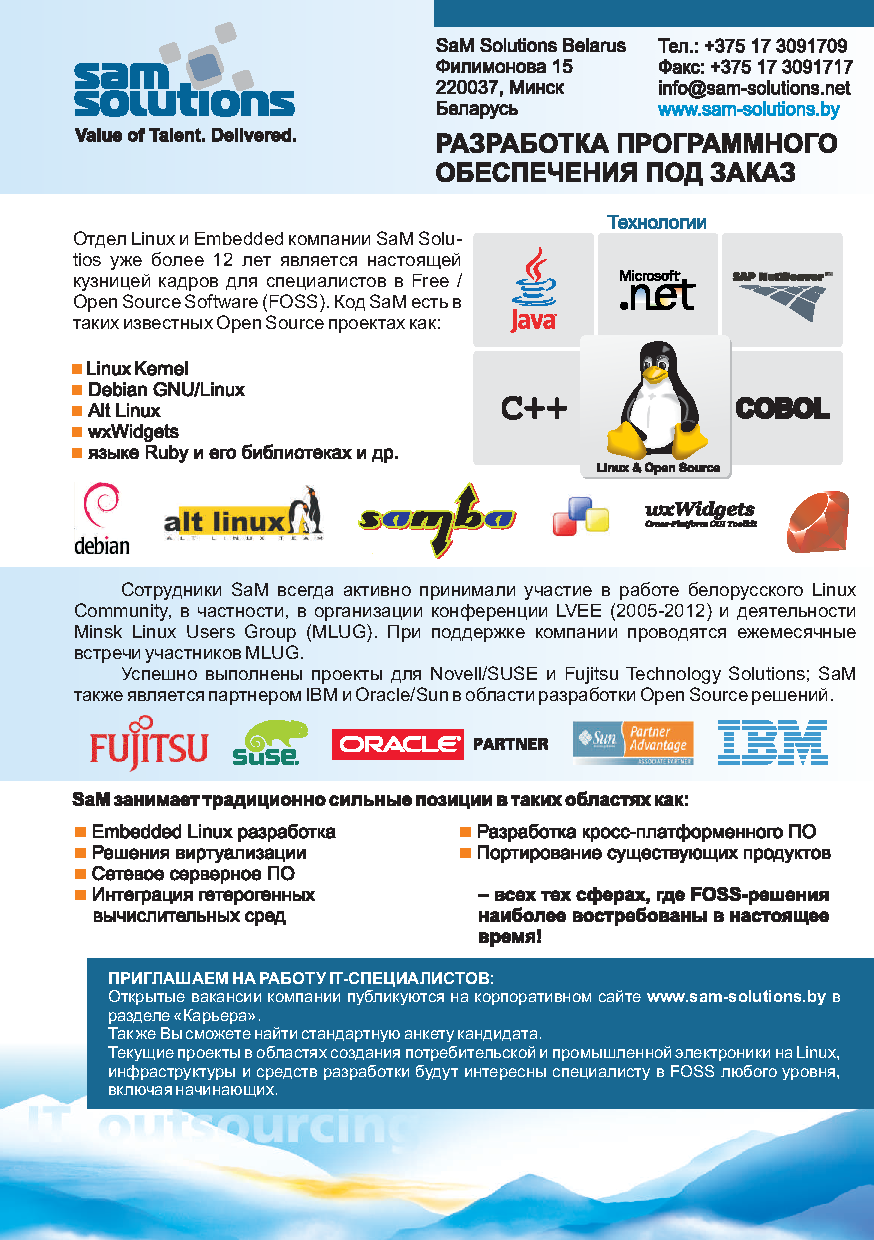
\includegraphics[height=11.8cm]{48_spons_sams.pdf}
\end{figure}
\end{document}



%\documentclass[10pt, a5paper]{article}
\usepackage{pdfpages}
\usepackage{parallel}
\usepackage[T2A]{fontenc}
\usepackage{ucs}
\usepackage[utf8x]{inputenc}
\usepackage[polish,english,russian]{babel}
\usepackage{hyperref}
\usepackage{rotating}
\usepackage[inner=2cm,top=1.8cm,outer=2cm,bottom=2.3cm,nohead]{geometry}
\usepackage{listings}
\usepackage{graphicx}
\usepackage{wrapfig}
\usepackage{longtable}
\usepackage{indentfirst}
\usepackage{array}
\newcolumntype{P}[1]{>{\raggedright\arraybackslash}p{#1}}
\frenchspacing
\usepackage{fixltx2e} %text sub- and superscripts
\usepackage{icomma} % коскі ў матэматычным рэжыме
\PreloadUnicodePage{4}

\newcommand{\longpage}{\enlargethispage{\baselineskip}}
\newcommand{\shortpage}{\enlargethispage{-\baselineskip}}

\def\switchlang#1{\expandafter\csname switchlang#1\endcsname}
\def\switchlangbe{
\let\saverefname=\refname%
\def\refname{Літаратура}%
\def\figurename{Іл.}%
}
\def\switchlangen{
\let\saverefname=\refname%
\def\refname{References}%
\def\figurename{Fig.}%
}
\def\switchlangru{
\let\saverefname=\refname%
\let\savefigurename=\figurename%
\def\refname{Литература}%
\def\figurename{Рис.}%
}

\hyphenation{admi-ni-stra-tive}
\hyphenation{ex-pe-ri-ence}
\hyphenation{fle-xi-bi-li-ty}
\hyphenation{Py-thon}
\hyphenation{ma-the-ma-ti-cal}
\hyphenation{re-ported}
\hyphenation{imp-le-menta-tions}
\hyphenation{pro-vides}
\hyphenation{en-gi-neering}
\hyphenation{com-pa-ti-bi-li-ty}
\hyphenation{im-pos-sible}
\hyphenation{desk-top}
\hyphenation{elec-tro-nic}
\hyphenation{com-pa-ny}
\hyphenation{de-ve-lop-ment}
\hyphenation{de-ve-loping}
\hyphenation{de-ve-lop}
\hyphenation{da-ta-ba-se}
\hyphenation{plat-forms}
\hyphenation{or-ga-ni-za-tion}
\hyphenation{pro-gramming}
\hyphenation{in-stru-ments}
\hyphenation{Li-nux}
\hyphenation{sour-ce}
\hyphenation{en-vi-ron-ment}
\hyphenation{Te-le-pathy}
\hyphenation{Li-nux-ov-ka}
\hyphenation{Open-BSD}
\hyphenation{Free-BSD}
\hyphenation{men-ti-on-ed}
\hyphenation{app-li-ca-tion}

\def\progref!#1!{\texttt{#1}}
\renewcommand{\arraystretch}{2} %Іначай формулы ў матрыцы зліпаюцца з лініямі
\usepackage{array}

\def\interview #1 (#2), #3, #4, #5\par{

\section[#1, #3, #4]{#1 -- #3, #4}
\def\qname{LVEE}
\def\aname{#1}
\def\q ##1\par{{\noindent \bf \qname: ##1 }\par}
\def\a{{\noindent \bf \aname: } \def\qname{L}\def\aname{#2}}
}

\def\interview* #1 (#2), #3, #4, #5\par{

\section*{#1\\{\small\rm #3, #4. #5}}

\def\qname{LVEE}
\def\aname{#1}
\def\q ##1\par{{\noindent \bf \qname: ##1 }\par}
\def\a{{\noindent \bf \aname: } \def\qname{L}\def\aname{#2}}
}

%\frenchspacing
\begin{document}
\title{Голос спонсора: ITS Partner}
%\author{}
\date{}
\maketitle

~

\newpage

~

\end{document}

%\documentclass[10pt, a5paper]{article}
\usepackage{pdfpages}
\usepackage{parallel}
\usepackage[T2A]{fontenc}
\usepackage{ucs}
\usepackage[utf8x]{inputenc}
\usepackage[polish,english,russian]{babel}
\usepackage{hyperref}
\usepackage{rotating}
\usepackage[inner=2cm,top=1.8cm,outer=2cm,bottom=2.3cm,nohead]{geometry}
\usepackage{listings}
\usepackage{graphicx}
\usepackage{wrapfig}
\usepackage{longtable}
\usepackage{indentfirst}
\usepackage{array}
\newcolumntype{P}[1]{>{\raggedright\arraybackslash}p{#1}}
\frenchspacing
\usepackage{fixltx2e} %text sub- and superscripts
\usepackage{icomma} % коскі ў матэматычным рэжыме
\PreloadUnicodePage{4}

\newcommand{\longpage}{\enlargethispage{\baselineskip}}
\newcommand{\shortpage}{\enlargethispage{-\baselineskip}}

\def\switchlang#1{\expandafter\csname switchlang#1\endcsname}
\def\switchlangbe{
\let\saverefname=\refname%
\def\refname{Літаратура}%
\def\figurename{Іл.}%
}
\def\switchlangen{
\let\saverefname=\refname%
\def\refname{References}%
\def\figurename{Fig.}%
}
\def\switchlangru{
\let\saverefname=\refname%
\let\savefigurename=\figurename%
\def\refname{Литература}%
\def\figurename{Рис.}%
}

\hyphenation{admi-ni-stra-tive}
\hyphenation{ex-pe-ri-ence}
\hyphenation{fle-xi-bi-li-ty}
\hyphenation{Py-thon}
\hyphenation{ma-the-ma-ti-cal}
\hyphenation{re-ported}
\hyphenation{imp-le-menta-tions}
\hyphenation{pro-vides}
\hyphenation{en-gi-neering}
\hyphenation{com-pa-ti-bi-li-ty}
\hyphenation{im-pos-sible}
\hyphenation{desk-top}
\hyphenation{elec-tro-nic}
\hyphenation{com-pa-ny}
\hyphenation{de-ve-lop-ment}
\hyphenation{de-ve-loping}
\hyphenation{de-ve-lop}
\hyphenation{da-ta-ba-se}
\hyphenation{plat-forms}
\hyphenation{or-ga-ni-za-tion}
\hyphenation{pro-gramming}
\hyphenation{in-stru-ments}
\hyphenation{Li-nux}
\hyphenation{sour-ce}
\hyphenation{en-vi-ron-ment}
\hyphenation{Te-le-pathy}
\hyphenation{Li-nux-ov-ka}
\hyphenation{Open-BSD}
\hyphenation{Free-BSD}
\hyphenation{men-ti-on-ed}
\hyphenation{app-li-ca-tion}

\def\progref!#1!{\texttt{#1}}
\renewcommand{\arraystretch}{2} %Іначай формулы ў матрыцы зліпаюцца з лініямі
\usepackage{array}

\def\interview #1 (#2), #3, #4, #5\par{

\section[#1, #3, #4]{#1 -- #3, #4}
\def\qname{LVEE}
\def\aname{#1}
\def\q ##1\par{{\noindent \bf \qname: ##1 }\par}
\def\a{{\noindent \bf \aname: } \def\qname{L}\def\aname{#2}}
}

\def\interview* #1 (#2), #3, #4, #5\par{

\section*{#1\\{\small\rm #3, #4. #5}}

\def\qname{LVEE}
\def\aname{#1}
\def\q ##1\par{{\noindent \bf \qname: ##1 }\par}
\def\a{{\noindent \bf \aname: } \def\qname{L}\def\aname{#2}}
}

%\frenchspacing
\begin{document}
\title{Голос спонсора: mycloud.by}
%\author{}
\date{}
\maketitle

~


\end{document}

\documentclass[10pt, a5paper]{article}
\usepackage{pdfpages}
\usepackage{parallel}
\usepackage[T2A]{fontenc}
\usepackage{ucs}
\usepackage[utf8x]{inputenc}
\usepackage[polish,english,russian]{babel}
\usepackage{hyperref}
\usepackage{rotating}
\usepackage[inner=2cm,top=1.8cm,outer=2cm,bottom=2.3cm,nohead]{geometry}
\usepackage{listings}
\usepackage{graphicx}
\usepackage{wrapfig}
\usepackage{longtable}
\usepackage{indentfirst}
\usepackage{array}
\newcolumntype{P}[1]{>{\raggedright\arraybackslash}p{#1}}
\frenchspacing
\usepackage{fixltx2e} %text sub- and superscripts
\usepackage{icomma} % коскі ў матэматычным рэжыме
\PreloadUnicodePage{4}

\newcommand{\longpage}{\enlargethispage{\baselineskip}}
\newcommand{\shortpage}{\enlargethispage{-\baselineskip}}

\def\switchlang#1{\expandafter\csname switchlang#1\endcsname}
\def\switchlangbe{
\let\saverefname=\refname%
\def\refname{Літаратура}%
\def\figurename{Іл.}%
}
\def\switchlangen{
\let\saverefname=\refname%
\def\refname{References}%
\def\figurename{Fig.}%
}
\def\switchlangru{
\let\saverefname=\refname%
\let\savefigurename=\figurename%
\def\refname{Литература}%
\def\figurename{Рис.}%
}

\hyphenation{admi-ni-stra-tive}
\hyphenation{ex-pe-ri-ence}
\hyphenation{fle-xi-bi-li-ty}
\hyphenation{Py-thon}
\hyphenation{ma-the-ma-ti-cal}
\hyphenation{re-ported}
\hyphenation{imp-le-menta-tions}
\hyphenation{pro-vides}
\hyphenation{en-gi-neering}
\hyphenation{com-pa-ti-bi-li-ty}
\hyphenation{im-pos-sible}
\hyphenation{desk-top}
\hyphenation{elec-tro-nic}
\hyphenation{com-pa-ny}
\hyphenation{de-ve-lop-ment}
\hyphenation{de-ve-loping}
\hyphenation{de-ve-lop}
\hyphenation{da-ta-ba-se}
\hyphenation{plat-forms}
\hyphenation{or-ga-ni-za-tion}
\hyphenation{pro-gramming}
\hyphenation{in-stru-ments}
\hyphenation{Li-nux}
\hyphenation{sour-ce}
\hyphenation{en-vi-ron-ment}
\hyphenation{Te-le-pathy}
\hyphenation{Li-nux-ov-ka}
\hyphenation{Open-BSD}
\hyphenation{Free-BSD}
\hyphenation{men-ti-on-ed}
\hyphenation{app-li-ca-tion}

\def\progref!#1!{\texttt{#1}}
\renewcommand{\arraystretch}{2} %Іначай формулы ў матрыцы зліпаюцца з лініямі
\usepackage{array}

\def\interview #1 (#2), #3, #4, #5\par{

\section[#1, #3, #4]{#1 -- #3, #4}
\def\qname{LVEE}
\def\aname{#1}
\def\q ##1\par{{\noindent \bf \qname: ##1 }\par}
\def\a{{\noindent \bf \aname: } \def\qname{L}\def\aname{#2}}
}

\def\interview* #1 (#2), #3, #4, #5\par{

\section*{#1\\{\small\rm #3, #4. #5}}

\def\qname{LVEE}
\def\aname{#1}
\def\q ##1\par{{\noindent \bf \qname: ##1 }\par}
\def\a{{\noindent \bf \aname: } \def\qname{L}\def\aname{#2}}
}

%\switchlang{be}
%\usepackage{color}
\begin{document}
\title{Интервью с участниками}
%\author{}
\date{}
\maketitle

По традиции в сборник материалов входят интервью, в которых активные участники
сообщества open source делятся своим мнением о свободном ПО, открытых
технологиях, роли и месте свободных лицензий, рассказывают, как видят проблематику
свободных проектов. В этот раз, из-за англоязычности всех интервьюируемых, интервью приводятся на двух языках - английском и русском.

\section{Pawel Chojnacki "---  Варшава, Польша}
%\begin{figure}[ht]
%\centering{\includegraphics[width=4cm]{49_spons_altoros.jpg}}
%\end{figure}
\begin{Parallel}[p]{}{}
     \ParallelLText{%
      \selectlanguage{english}
{\noindent \bf LVEE: Can you briefly introduce yourself?}

{\noindent \bf Pawel Chojnacki:} My name is Pawel, I live in Warsaw. I used to be a part of Warsaw hackerspace; right now I'm not engaged in any organizational activity, may be beside the Global Innovation Gathering (\url{http://www.globalinnovationgathering.com}), a community which also involves hackering. I’m a web developer, a freelancer, a frontend professional doing some Open Access Science in the meantime. I deal a lot with open source in my professional activity. And in addition to that I’m giving cybersecurity lectures, an introduction to cybersecurity: what to store, why should you use Firefox and Chrome but not Internet Explorer and Safari.  And I work with open source every day.

{\noindent \bf L: How did you get acquainted with open source software? Do you remember?} 

{\noindent \bf P:}  I’ve started using Firefox very early in my life. It was the first year of Firefox existence, I don’t remember exactly which year it was. But I didn't consider it open source, I knew nothing about it. So my first conscious meeting with open source was related to GIMP graphic editor. I just wanted some program which had more options than Paint, and I didn’t want payed Photoshop version. That’s why I learned GIMP. I looked through one tutorial, and the second, and started learning to work with GIMP. Than I met some people speaking Polish who were interested in GIMP and helped them to found Polish Gimp Users' Forum (messaging board for Polish-speaking GIMP users). And from that I started reading and got very interested in Linux and the open source philosophy, and that was, I think, in mid school and high school. 

{\noindent \bf L: By the way, did you have some previous experience with Photoshop, before starting GIMP, or not?}

{\noindent \bf P:}  I didn't have any previous experience. Nothing with Photoshop, or Corel, or anything else.

{\noindent \bf L: It's an interesting question, because we know a lot of examples, when different previous experience had complicated people using GIMP more or less. And you have also mentioned Hackerspace. It’s a hackerspace in Warsaw?}

{\noindent \bf P:} Yeah. Warsaw hackerspace. 

{\noindent \bf L: The topic of hackerspace itself is rather interesting, because we have finally officially registered Hackerspace in Minsk some time ago. How long does it work in Warsaw?}

{\noindent \bf P:} Four or five years. I was in the board of hackerspace, and was basically driving it full time as a community manager, or whatever you want to call it, for several months. It was founded basically by some enthusiasts but got wheel speed when Warsaw University of Technology decided to shut down their experimental technology division and all people who wanted to experiment went to the hackerspace. And right now Warsaw hackerspace is a club. It’s typical members are people who have quite similar background from the Internet, who chat there… Even with a similar sense of humor. Those who like specific areas of IT, the security, administration, and who want to contribute to some projects or just to use technology for fun.

{\noindent \bf L: Usually hackerspace communities have strong connections with some open hardware projects: they are either developing their own or using some devices previously developed under such open hardware licenses. Perhaps there is the same situation in Warsaw, isn’t it?}

{\noindent \bf P:} We don’t have any projects that the hackerspace is creating as a hackerspace, but several members have created several hacks, for example way to install OpenWrt on specific devices which where unknown to be able of doing this.

Also there is some tool for gathering money from the members, just to send e-mails with reminders, and show current status. So hackerspace has some infrastructure. It is open but not necessary all of it is open source. 
 
A lot of things are based on Arduino, but I wouldn’t call it open hardware with us, as not all this things are documented and shared. But at least few things are.

{\noindent \bf L: At the very beginning open hardware was exotic, it was even supposed that open source licenses are good for software but not for hardware and other areas, like art. But well, later several really popular projects have appeared published under such licenses. How do you think, what's the reason of their success?}

{\noindent \bf P:} I think it is because they bring right now technology to the people who have open hardware which is also standartized.

Because right now you can take Arduino, take Raspberry Pi, and you can be sure that the most of software written for the one piece will work on any similar kind of chip, anywhere in the world. 

For example we have OpenBCI brain amplifier created by a small startup in US, which is becoming a new Arduino for brain amplifying, for just brain signal analysis which is also a very important for the community. There are a lot of other projects...

So they are bringing the costs down, as you don't have any kind of overprotection from company that puts control and keeps the prices  so that they are profitable. 

This hardware projects are just tools for sharing knowledge and for sharing technical experience using them as building blocks in practice.

{\noindent \bf L: Thank you. 
I think that open source is the most powerful in software areas nowadays, but with open hardware and open media like Wikipedia for example, or creative Commons materials online – perhaps together they are three most widely used open directions.}

{\noindent \bf P:} I think you forgot about one thing. You’ve mentioned the media as Creative Commons and Wikipedia, but there's also open access and open notebook at science. 

Right now I’m working on the scientific project of my own, creating it with the totally open notebook access, so that I’m commenting every step of my experiment, with use of open source tools. This approach allows people to replicate the experiment in same environment. If I actually had the equipment which would be open hardware, it could be much easier to actually replicate the data gathering.

{\noindent \bf L: It’s really interesting, as it’s not very easy to reproduce results of other researchers sometimes.
And open source software has some powerful positions in scientific research because it allows to see sources and control how where all the calculations really done. }

{\noindent \bf P:} Yes especially, but there also may be problems. I don't know if you have heard, recently we have lost about 40,000 articles regarding neurology and fMRI, because someone put the wrong code into scientific tools used to monitor them. 

The package itself was open source, but nobody was actively testing it, nobody was actively looking. So it's not only about saying “Hey this is open”, as universities are saying - “This piece of software is open, but please don't look at it because only we understand how it works”. 

Yes, you have to document it. You have to put it to open environment and encourage people to test it, to modify, to understand how it works.

If you are the the owner and the creator, and also the only person who understands how it works, it's not really the open source. Somebody has to look at it, somebody has to analyze it. If that would happened to the FMRI tools that where used around the world for the last 15 years, we could have all the knowledge gathered with this tools intact. But now we have to scrape basically the 15 years of neurology, because the software was faulty. It contains different statistical methods than it was supposed to...

{\noindent \bf L: And what is the role of community in supporting such projects? For example there is the known problem of open source projects with only one person who really knows their internals. If such person goes away for some reasons and abandons the development process, the project is in real trouble. So what about the problem of the community involvement in the development?}

{\noindent \bf P:}I believe that in case of some projects community has to be more involved, test something, develop harder. Even if sometimes there is no need in development… For example we have that issue with the set of statistical tests that nobody else is going to implement because they are working, they are fast, they are okay. But we still need someone who actually got stuck in the code. Those who got check it from time to time and notice if anything does go wrong. 

Basically university workers can be maintainers in some cases. I think that if there's nobody from the community to volunteer, nobody able to make some package of software – then we should start looking at the university's officials, asking universities to maintain that. Actually start paying the university researchers to maintain some software and respond to all the people who requires something or would like to ask some questions. 

I am speaking about employees, who would do it instead of working on some of their own projects. Because I know how this is in computational neuroscience in Warsaw, and in Poland. More than 60\% of people aren’t contributing to science. They are mostly just read that old papers and do not creating anything but useless pieces of software that only they can use, but no one else. It is waste of money that are going to the universities. If they are to be useful, they should become maintainers of the scientific packages, they should start analyzing them, they should start being responsible for how they work.

I believe that would be one of the best uses of university money. Universities have actually started networking, because with several neurological projects around Europe you are just creating the same feature over and over again in several different universities: the French are doing the same as Germans, the same as Italians, the same as Polish and the same as Russians.
 
What's the point of replicating involved in it - they fit the same problems and they hope for each other to solve that. 

     }
     \ParallelRText{%
       \selectlanguage{russian}
{\noindent \bf LVEE: Для начала, несколько слов о себе.}

{\noindent \bf Pawel Chojnacki:} Меня зовут Павел, я живу в Варшаве. Раньше активно участвовал в Варшавском Хакерспейсе; в настоящий момент организационной активностью не занимаюсь, ну может быть кроме Global Innovation Gathering (\url{http://www.globalinnovationgathering.com}), сообщество, связанное в том числе с хакерством. Я веб-разработчик, фрилансер, специалист по разработке фронтэнда, а кроме того занимаюсь наукой и открытым доступом (Open Access). Мне много приходится работать со свободным ПО в профессиональной деятельности. А еще я читаю лекции по компьютерной безопасности, такое введение в информационную безопасность: что хранить, почему использовать Firefox и Chrome, а не Internet Explorer или Safari. Ну и каждый день имею дело со свободным ПО.

{\noindent \bf L: Не вспомнишь, как ты вообще познакомился со свободным ПО?} 

{\noindent \bf P:}  Я начал пользоваться Firefox в очень раннем возрасте. Это был первый год существования Firefox как такового, сейчас не вспомню, в каком именно году. Но я не воспринимал его как свободное ПО, просто ничего об этом не знал. Так что первая сознательная встреча со свободным ПО была связана с графическим редактором GIMP. Мне была нужна какая-нибудь программа с б\'{о}льшими чем у Paint возможностями, и мне не хотелось иметь дело с платной версией Photoshop. Поэтому я изучил GIMP. Заглянул в один туториал, потом в другой, и начал учиться с ним работать. Затем я познакомился с польскоговорящими людьми, которые интересовались GIMP, и помог им создать Polish Gimp Users' Forum (площадку для польскоговорящих пользователей GIMP). И начиная с этого момента я стал читать, заинтересовался Linux и философией свободного ПО, думаю, это было в средних или старших классах. 

{\noindent \bf L: А кстати, у тебя уже был какой-то опыт работы в Photoshop до GIMP или нет?}

{\noindent \bf P:}  Никакого прежнего опыта. Ни с Photoshop, ни с Corel, ни с чем-либо ещё.

{\noindent \bf L: Это интересный вопрос, потому что есть достаточно примеров, когда предыдущий опыт с чем-то другим в той или иной степени осложнял людям изучение GIMP. Итак, ты упоминал хакерспейс. Это хакерспейс в Варшаве?}

{\noindent \bf P:} Да. Варшавский хакерспейс. 

{\noindent \bf L: Тема хакерспейса сама по себе интересна, потому что не так давно мы наконец официально зарегистрировали хакерспейс в Минске. Как долго он существует в Варшаве?}

{\noindent \bf P:} Четыре или пять лет. Я был в совете хакерспейса, несколько  месяцев фактически тянул его на себе на штатной основе в качестве комьюнити-менеджера, или как ещё можно назвать эту должность. Он был сначала основан несколькими энтузиастами, а раскрутился, когда в Варшавском технологическом университете закрылось экспериментальное технологическое отделение, и тога все, кто хотел заниматься экспериментами, отправились в хакерспейс. А сейчас Варшавский хакреспейс --- это клуб. Его типичные члены --- это люди со схожим опытом в Интернет, которые в нём общаются… Вплоть до схожего чувства юмора. Те, кому нравятся определённые области IT, безопасность, администрирование, кто хотел бы вносить вклад в некоторые проекты или просто возиться с технологиями ради собственного удовольствия.

{\noindent \bf L: Обычно комьюнити хакерспейсов имеют сильные связи с проектами свободного аппаратного обеспечния: разрабатывают что-то своё, или используют устройства, созданные ранее под свободными лицензиями. В Варшаве наверное такая же ситуация?}

{\noindent \bf P:} У нас нет проектов, создаваемых в хакерспейсе именно от имени хакерспейса, но некоторые члены были инициаторами некоторых хаков --- например, способ установить прошивку OpenWrt на некоторые устройства, для которых прежде ничего не было известно о такой возможности.

Ещё есть инструмент для сбора денег с участников: напоминания по e-mails и т.~д., отображение текущего статуса. Понятно, у хакерспейса есть определенная инфраструктура. Она открыта, но не обязательно является свободной вся целиком. 
 
Многие вещи построены на Arduino, но в нашем случае я не назвал бы это свободным аппаратным обеспечением, потому что не все проекты задокументированы и выложены в общий доступ. Но несколько --- да.

{\noindent \bf L: В самом начале свободное аппаратное обеспечение считалось экзотикой, считалось даже, что свободные лицензии хороши для программ, но не для аппаратуры и некоторых других областей, как например искусство. Но однако, позже появилось несколько действительно популярных проектов именно под такими лицензиями. Как ты думаешь, в чём причина их успеха?}

{\noindent \bf P:} Думаю, в том, что они прямо сейчас несут технологию людям, в распоряжении которых есть аппаратура, свободная и при этом стандартизованная.

Прямо сейчас можно взять Arduino или Raspberry Pi и быть уверенным, что б\'{о}льшая часть ПО, написанного для одного устройства, будет работать на таком же чипе в любой точке планеты. 

Например, существует усилитель электрической активности мозга OpenBCI, созданный небольшим стартапом в США, который становится новым Arduino эля энцефалографии, для анализа сигналов мозга, и это тоже очень важно для комьюнити. Есть много других проектов...

Они снижают затраты, потому что нет никакой избыточной защиты от компаний которые всё контролируют и должны поддерживать цены на таком уровне, чтобы сохранить прибыльность. 

Эти аппаратные проекты --- просто инструменты, которые позволяют делиться знаниями и техническим опытом, используя их на практике в качестве готовых блоков.

{\noindent \bf L: Спасибо. 
Думаю, на текущий момент свободные технологии наиболее сильны в области ПО, аппаратного обеспечения и свободных медиа, таких как Википедия, например, или Creative Commons --- пожалуй, вместе это три наиболее сильные направления.}

{\noindent \bf P:} Я думаю, ты забыл одну важную вещь. Ты упомянул свободные медиа, такие как Creative Commons и Википедия, Но есть ведь еще в сфере науки и материалы с открытым доступом, и открытые лабораторные журналы (open notebook). 

Прямо сейчас я работаю над собственным научным проектом, создаю его в режиме открытого журнала, комментирую с помощью свободных инструментов каждый шаг эксперимента. Такой подход позволяет людям воспроизвести эксперимент в аналогичных условиях. И будь у меня оборудование, распространяемое на условиях свободных лицензий, было бы намного легче воспроизвести сбор данных.

{\noindent \bf L: Это очень интересная тема, результаты других исследователей вообще бывает не так уж легко воспроизвести.
And open source software has some powerful positions in scientific research because it allows to see sources and control how where all the calculations really done. }

{\noindent \bf P:} Yes especially, but there also may be problems. I don't know if you have heard, recently we have lost about 40,000 articles regarding neurology and fMRI, because someone put the wrong code into scientific tools used to monitor them. 

The package itself was open source, but nobody was actively testing it, nobody was actively looking. So it's not only about saying “Hey this is open”, as universities are saying - “This piece of software is open, but please don't look at it because only we understand how it works”. 

Yes, you have to document it. You have to put it to open environment and encourage people to test it, to modify, to understand how it works.

If you are the the owner and the creator, and also the only person who understands how it works, it's not really the open source. Somebody has to look at it, somebody has to analyze it. If that would happened to the FMRI tools that where used around the world for the last 15 years, we could have all the knowledge gathered with this tools intact. But now we have to scrape basically the 15 years of neurology, because the software was faulty. It contains different statistical methods than it was supposed to...

{\noindent \bf L: And what is the role of community in supporting such projects? For example there is the known problem of open source projects with only one person who really knows their internals. If such person goes away for some reasons and abandons the development process, the project is in real trouble. So what about the problem of the community involvement in the development?}

{\noindent \bf P:}I believe that in case of some projects community has to be more involved, test something, develop harder. Even if sometimes there is no need in development… For example we have that issue with the set of statistical tests that nobody else is going to implement because they are working, they are fast, they are okay. But we still need someone who actually got stuck in the code. Those who got check it from time to time and notice if anything does go wrong. 

Basically university workers can be maintainers in some cases. I think that if there's nobody from the community to volunteer, nobody able to make some package of software – then we should start looking at the university's officials, asking universities to maintain that. Actually start paying the university researchers to maintain some software and respond to all the people who requires something or would like to ask some questions. 

I am speaking about employees, who would do it instead of working on some of their own projects. Because I know how this is in computational neuroscience in Warsaw, and in Poland. More than 60\% of people aren’t contributing to science. They are mostly just read that old papers and do not creating anything but useless pieces of software that only they can use, but no one else. It is waste of money that are going to the universities. If they are to be useful, they should become maintainers of the scientific packages, they should start analyzing them, they should start being responsible for how they work.

I believe that would be one of the best uses of university money. Universities have actually started networking, because with several neurological projects around Europe you are just creating the same feature over and over again in several different universities: the French are doing the same as Germans, the same as Italians, the same as Polish and the same as Russians.
 
What's the point of replicating involved in it - they fit the same problems and they hope for each other to solve that. 


     }
   \end{Parallel}







\section{Мiхаiл Волчак "---  Мiнск, Беларусь}
%\begin{figure}[ht]
%\centering{\includegraphics[width=4cm]{49_spons_altoros.jpg}}
%\end{figure}

{\noindent \bf LVEE: Ты прымаў удзел у некалькіх папярэдніх LVEE ў досыць розных амплуа: ад прэзентацыі беларускай партыі піратаў да воркшопа па меш-сетках. Як бы ты ідэнтыфікаваў сябе ў першую чаргу?
}

{\noindent \bf Мiхаiл Волчак:} Перш за ўсё для мне цікавыя такія праекты, у якіх удзельнічае супольнасць, таму што, супольнасць дае разнастайнасць, а я лічу што разнастайнасць "--- гэта такая базавая ўмова для развіцця. Гэта датычыцца розных праектаў, у тым ліку і развіцця размеркаваных меш-сетак. Але вядома я "--- пірат.

{\noindent \bf L: Які менавіта тэрмін ты ўкладаеш у слова «пірат»?}

{\noindent \bf М:} Піраты для мяне "--- гэта пэўная ідэалогія, калі Інтэрнэт на сваю карысць выкарыстоўваюць людзі, а не «крывавы карпарэйшн», напрыклад\ldots Гэта пірацкая палітычная ідэалогія, якая зараз узнікае, яе тэзіс, калі лаканічна, дэмакратыя з выкарыстаннем лічбавых сродкаў, праграмных і апаратных.




{\noindent \bf L: І гэтая твая цікавасць неяк перасякаецца з вольнымі ліцэнзіямі і кантэнтам, да якіх ты маеш непасрэднае дачыненне?} 

{\noindent \bf М:}  Свабодны кантэнт у нашу эпоху ведаў, пост-інфармацыйную эпоху\ldots

{\noindent \bf L: А пост-інфармацыйная, гэта?..}

{\noindent \bf М:}  Усе кажуць што мы ў інфармацыйнай, а насамрэч зараз важна пост-інфармацыя, калі мы не толькі ўспрымаем дадзеныя, мы іх ўмеем пераўтвараць у веды. Для спажыўцоў "--- інфармацыйная. Але iнфармацыя гэта не мэта, а сродак або інструмент.

{\noindent \bf L: І як гэта і пірацтва звязана са свабодным кантэнтам?}

{\noindent \bf М:} А як пірацтва звязана с кантэнтам? Кантэнт можна не толькі спажываць, а яго можна яшчэ змяняць, i гэта асноўны падыход, які мне блізкі. Яго можа зменяць кожны, калі мы заходзім у сеціва і маем там вікі ў сваіх свабодных праектах, і такім часам мы не проста спажыўцы, а сустваральнікі. Сустварэнне "--- гэта такая важная штука для любога апенсорса і ўвогуле любой супольнасці, якая хоча развівацца. Ўключаць новае ў свой дыскурс.

Першы кампанент "--- гэта сумесны ўдзел і магчымасць змяняць кантэнт, і другі кампанент "--- абараніць гэты кантэнт у эпоху, калі яго могуць прыватызаваць. Першапачатковую маёмасць супольнасці часам могуць прыватызаваць праз такія інструменты, як інтэлектуальная ўласнасць, гэта цэлы набор законаў, які дазваляе эканамічным суб'ектам, фірмам там, вялікім, малым "--- прысвойваць. Другі бок "--- гэта юрыдычнае спараджэнне свабоднага кантэнта, так званыя свабодныя ліцэнзіі, якія мы маем. GNU, Creative Commons (Творчыя Суполкі), яшчэ шэраг. Пад свабодай кантэнту мы маем тое ж самае, што з сафтом, тыя знакамітыя рычардавскія свабоды: свабода вывучаць, змяняць і распаўсюджваць. Калі ў кантэнту адна свабода знікае "--- знікае і цэласнае разуменне гэтай свабоды. Палітычныя піраты на сёння гэта разумеюць. Напрыклад, з забаронай распаўсюджвання знікае магчымасць арганічнага развіцця супольнасці. Карпаратыўнае развіццё можа мець месца, але тады арганічнасць знікае\ldots


{\noindent \bf L: Аднак, твая цікавасць да свабодных ліцэнзіях з'явілася яшчэ раней? Як гэта было?}

{\noindent \bf М:} Упершыню я пачуў пра гэта дзесьці ў годзе 2009-2010. У той перыяд, калі я пачаў больш глыбока разумець вікі-тэнхалогію і пачаў працаваць. Гэта прыйшло ад сафта. Я доўга мучыўся ад дыхатаміі Wіndows-Lіnux, першы мой Lіnux быў у 1999 годзе, я яго роўна на паўгадзіны устанавіў\ldots

{\noindent \bf L: Які дыстрыбутыў?}

{\noindent \bf М:} Asp Lіnux, там было некалькі дыскаў, якія я засоўваў і высоўваў "--- проста набыў дыскі і пачаў з імі іграцца\ldots Але потым была Kubuntu дзесь у 2010 годзе, у мяне стабільна сталі дзве сістэмы. Другі крок гэта былi web-applіcatіon, Drupal. Я актыўна удзельнічаў у Drupal-супольнасці, актыўна вывучаў Drupal і пасля пачаў чытаць лiцэнзiйныя дамовы GNU GPL, разоў пяць пачынаў чытаць і не заканчваў, але мне спадабаўся канцэпт. Канцэпт не з узору легальнасцi насамрэч "--- тое, што ён выяўляўся не для вырашэння задач камерцыі, а для вырашэння задач супольнасці. Я ў Drupal-супольнасць пагрузіўся не як спажывец праграмы, ці там кода, а як удзельнік, ну і тады я пачаў вывучаць пакеты, з якімі яны працуюць, і тады пакацілася. 

Ліцэнзійныя прынцыпы рэфлексуюць прынцыпы супольнасці, і калі ты адымаеш ад супольнасці штосьці з гэтых прынцыпаў, атрымліваецца нейкая карпаратыўная культура, а калі ты працуеш з трыма свабодамі, атрымліваецца супольнасць. А потым з Creatіve Commons платнічок пайшоў ў 2012 годзе. Я чытаў шмат кніг пра капірайт, і так арганічна гэта пайшло туды\ldots
 

{\noindent \bf L: Лоўрэнс Лессіг распіярыў?}

{\noindent \bf М:} Ведаеш, магчыма ад яго пайшлі некаторыя словы. Яго «Свабодная культура» дала мне нейкі стартавы слоўнікавы запас, на які можна было абапірацца далей.

{\noindent \bf L: А раскажы трохі аб Вікіпедыі. Пра сваё знаёмства з самой тэхналогіяй, падыходам, калі кам'юніці рэгулюе артыкулы.}

{\noindent \bf М:} Знаёмства адбылося практычна. Напісаў артыкул, яго праз не\-калькі хвілін выдалілі, а я на яго патраціў тры дні. Тады я зрабіў паўзу, таму што не разумеў, як працуе гэта супольнасць\ldots Вядома, я выкарыстоўваў той жа падыход, які выкарыстоўваў у Drupal-супольнасці, але яно не спрацавала. І хутчэй па культурна-палі\-тычным плане\ldots

{\noindent \bf L: Як гэта?}

{\noindent \bf М:} Я напісаў артыкул, які не адпавядаў крытэрыям значнасці для рускай вікіпедыі\ldots Потым я зноў пачаў пісаць, напісаў артыкул у беларускай вікіпедыі, яго заапрувілі і жыццё пайшло\ldots І вось у гэты момант, калі заапрувілі (быў статус «на вычытку» і раптам змяніўся) "--- мне стала цікава, як адбываецца самарэгуляцыя, як кантэнт застаецца рэлевантным.

{\noindent \bf L: У нейкім сэнсе самарэгуляцыю ты адчуў на сабе, пры першай спробе\ldots}

{\noindent \bf М:} Не зусім так. Спачатку мне здавалася, што гэта самарэгуляцыя, але потым прыйшло разуменне. Моўныя раздзелы, якія маюць 100-200 тысяч артыкулаў, выкарыстоўваюць стратэгію «набраць колькасць», калі прымаюцца любыя артыкулы, якія маюць 2-3 крыніцы. Калі раздзел перасякае рысу 500-600 тысяч, яны трохі змяняюць стратэгію,але вось гэтая свабода дадавання колькасці існуе. А калі яны перасякаюць мільён, або 800-900 тысяч, яны кардынальна мяняюць стратэгію і павялічваюць крытэрый значнасці. Такую стратэгію спачатку выкарыстоўвала і руская вікіпедыя, але пасля гэтага парога яны пачалі касіць усё, што нязначна для Расіі і выкарыстоўваюць тую ж стратэгію для беларускіх артыкулаў. Іншымі словамі, для “свадобных” ведаў у рувікі выкарыстоўваюцца геаграфічныя і культурна-палітычныя межы.


{\noindent \bf L: Патлумач гэты момант.}

{\noindent \bf М:} Ну, мы ж з большасці рускамоўныя, таму і пішам там.

У вікі-супольнасці ёсць 5 прынцыпаў асноўных, адзін з іх "--- крытэрый значнасці, notable sources, і ў многіх вялікіх раздзелах яна дэфармавалася ў крытэрый мега-якасці, які стварае такі парог уваходу, што ў невялікіх супольнасцяў не знойдзецца столькі спецыялістаў, якія будуць пісаць на адмысловую тэму. Атрымліваецца што невялікая супольнасць, напрыклад беларуская, якая прымае такія ж стандарты, якія існуюць у польскай або ў рускай wіkі (у польскай мякчэй) "--- узнікае такі парог уваходу, што пачаткоўца, які захоча нешта напісаць, выкідваюць з удзелу.


{\noindent \bf L: А чаму такі падыход не назіраецца ў ангельскай?}

{\noindent \bf М:} Да, з ангельскай вікі такія праблемы не ўзнікалі, я публікаваў нават такі эксперыментальны матэрыял, які быў бы з рускай выключаны з тымі крытэрыямі. Кожная супольнасць, нават і анлайнавая, рэфлексуе, як бы ты не хацеў называць яе анлайнавай, пэўную мадэль лакацыі\ldots Ангельская "--- выключэнне, таму што гэта вельмі глабальная супольнасць, яна больш інтэрнацыянальная, там і Еўропа, і Амерыка, і Азія. Ўсюды англійскае камьюніці, і таму там культурнага рэлятывізму або нейкай палітычнай скіраванасці не існуе.
 
{\noindent \bf L: І напрыканцы, як ты ўяўляеш сабе перспектывы адкрытых ліцэнзій ў вобласці, не звязанай з софтам: у open media, open hardware?}

{\noindent \bf М:} Асноўная праблема кантэнтных і сафтовых ліцэнзій "--- тое, што яны не арыгінальныя для трох чвэрцей гэтай планеты. У іх вельмі класная задума, як хакнуць залішнія абмежаванні, напрыклад, капірайта, але яны вельмі арганічна глядзяцца ў краіне, дзе капірайт найбольш развіты і стаў часткай штодзеннага жыцця для многіх. Для Беларусі гэта нехарактэрна, Беларусь ніколі не была краінай, дзе капірайт вельмі прывіваўся\ldots Ад Францыска Скарыны, які быў піратам і правозіў кантрабанднае абсталяванне праз польскую мяжу для распаўсюду свабодных ведаў у Вялікім Княстве Літоўскім.


{\noindent \bf L: ?!}

{\noindent \bf М:} Так, яго двойчы затрымлівалі, і толькі на трэці раз яму ўдалося правезці гэта hardware, і толькі пасля гэтага ён змог заняцца тут кнігадрукаваннем\ldots Умоўна кажучы, гэтая ліцэнзійная фішка павінна перасэнсавацца нашым грамадствам, і ўсімі не Western Europe і амерыканскімі супольнасцямі. Заходняя Еўропа "--- гэта індывідуалістычны падыход да ўсяго, а open source "--- гэта communіty ownershіp, tradіtіonal knowledge, традыцыйныя веды, калі усё “племя” нешта ведае, і ніхто не робіць гэтыя веды прапрыятарнымі, каб нажыцца. Сеткавыя супольнасці зараз працуюць па гэтым жа прынцыпе як плямёны там\ldots з Лацінскай Амерыкі ці Аўстраліі, і таму тут пытанне з гэтымі ліцэнзіямі, якія індывідуальна накіраваныя.

{\noindent \bf L: Але яны досыць паспяхова прымяняюцца?}

{\noindent \bf М:} Не зусім так. Спачатку мне здавалася, што гэта самарэгуляцыя, але потым прыйшло разуменне. Моўныя раздзелы, якія маюць 100-200 тысяч артыкулаў, выкарыстоўваюць стратэгію «набраць колькасць», калі прымаюцца любыя артыкулы, якія маюць 2-3 крыніцы. Калі раздзел перасякае рысу 500-600 тысяч, яны трохі змяняюць стратэгію,але вось гэтая свабода дадавання колькасці існуе. А калі яны перасякаюць мільён, або 800-900 тысяч, яны кардынальна мяняюць стратэгію і павялічваюць крытэрый значнасці. Такую стратэгію спачатку выкарыстоўвала і руская вікіпедыя, але пасля гэтага парога яны пачалі касіць усё, што нязначна для Расіі і выкарыстоўваюць тую ж стратэгію для беларускіх артыкулаў. Іншымі словамі, для “свадобных” ведаў у рувікі выкарыстоўваюцца геаграфічныя і культурна-палітычныя межы.


{\noindent \bf L: Тут выразна чутны голас пірацкай партыі :-)}

{\noindent \bf М:} Я пакуль спрабую перасэнсаваць гэтае пытанне\ldots Я за тое, каб гэтыя ліцэнзіі прысутнічалі, я сам прасоўваю ліцензіі Creative Com\-mons ў Беларусі. Але калі займаешся іх прамоўшнам\ldots Так, пад вікіпедыяй ёсць Creatіve Commons, але 90\% вікіпедыстаў разумеюць гэтую ліцэнзію хутчэй праз паводзіны ў супольнасці, а не ў юрыдычным плане. Паовдзіны супольнасці фарміруюць правілы "--- змест гэтых ліцэнзій, а не наадварот. Гэта для мяне важный момант\ldots

А ліцэнзіі на жалеза "--- гэта больш накшталт патэнтаў. У патэнтаў ёсць адзін плюс\ldots У іх ёсць шмат мінусаў, але адзін плюс, якому пакуль не прыдумана альтэрнатыва. Яны ўсё ўключаюць у адну базу дадзеных, якую чалавек можа праглядаць. Вось калі open source community, якое працуе з hardware, выпрацуе нейкі падобны механізм з класіфікатарам, катэгарызацыяй "--- тады гэта можа быць годнай альтэрнатывай, але пакуль такога механізму няма. Гэта выклік "--- ці могуць актывісты open hardware такое зрабіць, але такое трэба. Першая ўмова росту папулярнасці вольных ліцэнзій для hardware "--- гэта стварыць сістэму, якая будзе больш эфектыўная, больш адкрытая, чым патэнтнае бюро, патэнтныя офісы па розных краінах.

\switchlang{ru}  

\section{Даниэль Надь "---  Будапешт, Венгрия}
%\begin{figure}[ht]
%\centering{\includegraphics[width=4cm]{49_spons_altoros.jpg}}
%\end{figure}

{\noindent \bf LVEE: Поскольку нынешние интервью связаны с комьюни\-ти-ориентированными и свободными технологиями за пределами непосредственно свободного программного обеспечения "--- поговорим о криптовалютах. Как возник твой интерес к этой сфере?}

{\noindent \bf Даниэль Надь:} Это уходит корнями в глубокое детство. В 1984 году была выпущена такая компьютерная игра, Elite...\ldots 

{\noindent \bf L: Ух ты! Всё началось с неё?}

{\noindent \bf Д:} Вот, ты её тоже помнишь. Я в неё вложил "--- т. е. закопал "--- многие тысячи часов, наверное. И когда уже появился Интернет, у меня была такая мечта "--- сделать что-то похожее, но для большого количества игроков. Сейчас уже такие игры существуют, а когда я занимался этим  своим юношеским проектом "--- тогда возникали две проблемы. Во-первых, достаточно быстро стало ясно, что на централизованном сервере хранить все это очень затратно. Хотелось использовать вычислительные мощности клиентов, сделать какую-то распределенную систему. А во-вторых, я заметил, что в Elite наступал такой момент, когда у игрока становилось очень много денег, и игра из-за этого делалась несколько скучной. Я задумался, почему так не случается в жизни, начал читать про денежную систему "--- как это работает, что такое деньги вообще, почему, например, в игре никогда не случается так, что у меня есть какой-то товар, а у покупателей на космической станции нет денег\ldots

{\noindent \bf L: Действительно :)} 

{\noindent \bf Д:} ...а в реальном мире это достаточно частая ситуация. В общем, я начал вчитываться в суть денег, потом наступил крах доткомов 2001 года, когда у многих появился интерес к этой теме, и появилось с кем об этом поговорить. Сначала я начал вчитываться в то, как можно вести распределенный бухгалтерский учет для большой онлайн-игры, а через некоторое время задумался: зачем это делать в игрушечном варианте, когда чего-то подобного миру не хватает по-настоящему. 

{\noindent \bf L: Как обстояли на тот момент дела с электронными платёжными системами?}

{\noindent \bf Д:}  В 1998 году в русскоязычном пространстве появился Webmoney, а за несколько лет до этого был DigiCash, так что ростки криптовалют "--- они появлялись в конце 90-х, а теоретические основы (академические статьи на эту тему) начали появляться ещё в 80-х.

{\noindent \bf L: А в распределенном, децентрализованном виде?}

{\noindent \bf Д:} Всем хотелось децентрализации. Это был такой Святой Грааль, который всем хотелось сделать. И, естественно, была проблема византийского консенсуса. Если описать простыми словами "--- это задача, как обеспечить, чтобы состояние бухгалтерского учета было для всех одинаково, с какой точки ни смотри на систему, т. е. чтобы всегда сохранялась целостность. Это была достаточно сложная проблема, и хорошего практического решения она не имела, пока вдруг из ниоткуда не появился Bitcoin.

{\noindent \bf L:А блокчейн?}

{\noindent \bf Д:} Он не существовал до Bitcoin. 

{\noindent \bf L: Насколько понимаю, распределенная децентрализованная система по идеологии и принципам достаточно близка открытому ПО. И что, Bitcoin оказался первой реально успешной системой электронных денег, по своим принципам родственной свободному ПО?}

{\noindent \bf Д:} Не сказал бы, что первой. Были свободные проекты до Bitcoin. И ePoint ведь тоже был основан на открытом ПО, и еще было много разных проектов. Это в начале двухтысячных была достаточно горячая тема, многие ею занимались, были разные эксперименты, но они были не очень успешны именно из-за той нерешенной проблемы, о которой мы только что говорили.

{\noindent \bf L: Кто первый сумел ее решить, тот завоевал мир?}

{\noindent \bf Д:} Да. Хотя я этот параметр и не очень высоко ценю, но тем не менее рыночная капитализация Bitcoin в разы превосходит рыночную капитализацию остальных криптовалют вместе взятых.

{\noindent \bf L: С технической точки зрения, со времён появления Bitcoin криптовалюты как-то развивались?}

{\noindent \bf Д:} Конечно. Есть разные направления развития. Кстати не все они положительные. Да и направление развития Bitcoin не совсем соответствует тем ожиданиям и предсказаниям, которые ему сопутствовали в 2009 году.  На сегодняшний день децентрализация Bitcoin во многом условна. На самом деле обработка транзакций происходит на достаточно маленьком количестве узлов, которое к тому же еще и сокращается.

{\noindent \bf L: И территориально, насколько я помню, есть проблема, что почти все они расположены там, где быстро делают микросхемы, и\ldots}

{\noindent \bf Д:} ...и где легко воровать электричество, называя вещи своими именами.

Когда эти проблемы Bitcoin стали более-менее очевидными, многие взялись их решать. Первая более-менее успешная альтернатива "--- Litecoin, базируется на коде Bitcoin, и тут как раз видно преимущество открытого ПО, потому что можно было не реализовывать всё с нуля, а просто взять Bitcoin и поправить там некоторые вещи, чтобы достичь тех целей, которые разработчики себе поставили. В случае Litecoin основной задачей была децентрализация майнинга. В отличие от ожиданий Сатоши Накамото, оказалось что идеальный майнер в Bitcoin "--- это не универсальный компьютер, а некая микросхема, созданная именно под эту задачу. И создатели Litecoin задались целью создать такой алгоритм майнинга, который лучше всего выполняется на компьютере общего назначения. Это им в какой-то степени удалось. 

А еще в тот момент, когда запустили Litecoin, люди уже были знакомы с Bitcoin, поэтому у этой системы не было ещё одной проблемы. Около трети общего количества биткоинов находится в руках максимум 18 юридических или физических лиц. Эта очень большая централизация денежной массы случилась из-за того, что в самом начале мало кто знал о Bitcoin, и ранние майнеры очень много себе намайнили. С Litecoin такой проблемы не было, т. к. когда его объявили, очень многие бросились заниматься майнингом. И сам майнинг там децентрализован благодаря тому, что очень долго не было (а по-моему, и до сих пор нет) специализированных микросхем. 

Это было первое развитие темы Bitcoin "--- достаточно успешный проект, у которого тоже существенная рыночная капитализация, и кроме того есть ещё некоторые преимущества перед Bitcoin. Например, существенно быстрее время блоков. 


{\noindent \bf L: Думаю, это нелишним будет пояснить.}

{\noindent \bf Д:} Для тех кто не знаком с основными принципами блокчейна, можно сказать, что Bitcoin "--- это такая большая публичная бухгалтерия, куда записываются все транзакции, и страница в этой бухгалтерской книге "--- это блок.

{\noindent \bf L: Копии всех страниц должны быть на каждом узле, и благодаря системе указателей с цифровыми подписями ни у кого нет возможности незаметно модифицировать часть блокчейна.}

{\noindent \bf Д:} Да. И пока транзакция не попала в эту общую книгу, она теоретически может быть ещё изменена или удалена. Транзакция становится точной и необратимой, когда попадает в этот децентрализованный распределенный блокчейн. В случае Bitcoin это занимает в среднем около 10 минут, а в случае Litecoin "--- 2.5 минуты. 

{\noindent \bf L: После этого были ещё похожие системы?}

{\noindent \bf Д:} Очень много. Многие пытались что-то улучшить. С технической точки зрения им это может быть и удалось, но в случае с криптовалютами очень силён эффект сети. Даже если какая-то криптовалюта по параметрам  лучше Bitcoin, для того, чтобы у нее появилась существенная база пользователей, она должна найти для себя нишу, потому что сам тот факт, что огромное количество людей и бизнесов пользуется Bitcoin, делает остальные альтернативы непривлекательными.
 
{\noindent \bf L: Кстати, по поводу блокчейна, который присутствует на всех узлах. Вроде бы криптовалюты считаются такими анонимными, но при этом все твои транзакции сохраняются навсегда в публичном доступе. Они вроде бы пока не привязаны к твоей персоне, но никогда нет гарантии что\ldots}

{\noindent \bf Д:} ...что кто-нибудь потом не привяжет.


{\noindent \bf L: Да. Так насколько корректно считать это способом анонимнизации платежей?}

{\noindent \bf Д:} По-моему, совершенно некорректно. Bitcoin я бы анонимным не назвал. Есть отдельные анонимизаторы, такие сервисы, принимающие грязные биткоины, а возвращающие отмытые. Потом есть, скажем так, теоретически разработанные технологии, при помощи которых можно создать действительно анонимную криптовалюту. Этим сейчас тоже занимаются люди, и думаю, это тоже одно из направлений, куда в будущем будут развиваться технологии.

{\noindent \bf L: По поводу анонимности. Получается, если какие-то правительства косо смотрят на Bitcoin по поводу возможности сокрытия доходов "--- то это скорее ошибочная точка зрения?}

{\noindent \bf Д:} Нет, с этим уже не соглашусь. Несмотря на то, что биткоины не очень сложно привязать к какому-то конкретному имени, их очень сложно отнять и очень сложно воспрепятствовать их движению. Само по себе использование Bitcoin еще не спасает в случае чего, но если у человека значительная часть сбережений в биткоинах "--- он, грубо говоря, бежит значительно быстрее в случае каких-то потрясений. Когда случаются какие-то финансовые катаклизмы, массовые неплатежи или финансовый кризис в банковской системе, тогда бывает паника, люди пытаются перемещать свои капиталы, но многим это не удаётся или удаётся только частично. И вот в этом случае Bitcoin очень сильно помогает "--- это было продемонстрировано в случае кипрского кризиса, потом греческого кризиса, последнее время в Восточной Европе тоже, в Украине, и в Беларуси тоже, по-моему, те кто сделал ставку на Bitcoin, не ошиблись. 

Но есть ещё и такое преимущество Bitcoin и вообще систем распределённого бухгалтерского учета: если надо, они достаточно хорошо сочетаются с системой налогообложения, контроля. Например, я сейчас получаю значительную часть моей прибыли в криптовалютах, получаю от фонда, фонд должен держать свою бухгалтерию открытой, тот факт что это получаю я, а не кто-то другой "--- это не секрет, я с этих денег конечно же плачу налоги. В налоговой было достаточно просто показать, что вот этот счет, вот транзакция "---  в общем, из-за этого не возникает подозрений, что где-то тут мошенничество или что я что-то скрываю. Т. е. если я хочу играть с открытыми картами "--- я имею такую возможность.

Подводя итог,  такой подход в значительной степени отдаёт контроль над средствами индивиду или организации, даёт возможность решать, какую часть своих операций держать в какой юрисдикции. Это ставит юрисдикции в положение конкуренции друг с другом.


{\noindent \bf L: Еще вопрос про применение блокчейна за пределами платёжных систем. Насколько понимаю, с тех пор появились и такие проекты?}

{\noindent \bf Д:} Да. Я работаю как раз над таким проектом. Сейчас наиболее известен и успешен среди таких проектов Etherium "--- проект, который действительно превратил распределенный бухгалтерский учет Bitcoin в распределенную базу данных общего назначения. Там можно хранить в блокчейне любые данные и записывать условия изменения этих данных на тьюринг-полном языке.
 То есть на этих данных можно проводить практически любые вычисления так, что все могут убедиться: действительно результатом этих вычислений стало то-то и то-то. Здесь открываются такие возможности, о которых даже трудно говорить. Это как пытаться в начале 80-х годов рассказать, что такое персональный компьютер. Подавляющее большинство будущих применений еще не видны из нашей перспективы, потому что их еще не изобрели.

{\noindent \bf L: Можешь привести хотя бы парочку примеров, случайно выбранных?}

{\noindent \bf Д:} Попытаюсь. Например, можно сделать страховку без страховой компании. Если какие-то люди хотят распределить между собой какие-то риски, они могут записать условие в умный контракт: тот, кто регулярно делал какие-то взносы и с ним что-то случилось, получает определённые деньги. Это записывается в контракт, и таким образом страхование становится распределенным и децентрализованным: нет страховой компании, есть только люди, которые между собой поделили риски. 

Или, что меня больше всего интересует "--- это общее пользование капиталом. Самое простое, то над чем я сейчас конкретно работаю "--- чтобы любой человек мог сдавать в аренду свои вычислительные ресурсы. В данном случае это хранение и передача данных,  такое распределенное хранилище, к которому любой человек может подключить свои накопители и зарабатывать на том, что его накопителями пользуются другие люди.

{\noindent \bf L: То есть мы говорим не строго о вычислительной мощности процессора, мы понимаем более широко.}

{\noindent \bf Д:} Да, более широко, но и процессор тоже. В будущем, я думаю, можно будет сдавать в аренду и процессор. Есть какая-то программа, которая записывается в блокчейн, и потом данные можно рассылать разным участникам, они эти данные будут обрабатывать. Конечно, должна быть некоторая избыточность. Если те же  самые данные два узла обработали иначе, автоматически без участия человека можно выяснить, кто из них обработал данные неправильно, и исключить этот узел. Можно, например, распределенно рендерить фильмы. Но это, мне кажется, только первые ласточки, это достаточно просто. А вот, например, есть такая проблема, что огромное количество капитала человечества существует в виде припаркованных автомобилей, которые ничего не делают, а просто загораживают дорогу.

{\noindent \bf L: Неожиданно.}

{\noindent \bf Д:} Из-за того, что мы друг другу не доверяем, я не могу подойти к какому-то припаркованному автомобилю, быстро доказать владельцу, что я надёжный и хороший человек и у меня есть достаточно сбережений, чтобы компенсировать ему ущерб, если я его машину сломаю. Несмотря на то что это так, я не могу легко и просто это доказать. Но при помощи блокчейн-технологий это все становится доказуемо: как репутация, так и финансовое положение. Можно сделать такую автоматическую систему, когда к любому автомобилю можно подойти, быстро доказать, что мне его можно дать в аренду, заплатить, поехать куда-то и там его оставить для следующего желающего. Таким образом, количество машин, которое должно существовать, оказывается значительно меньшим. Многим не нужно будет иметь собственный автомобиль. И мне кажется что в итоге от этого человечество станет значительно богачP:  90\% автомобилей не нужно будет производить, и эти мощности можно будет использовать для чего-то другого.

{\noindent \bf L: По существу, блокчейн "--- такой достаточно мощный механизм, который «перетащит» комьюнити-технолгоии в \linebreak осязаемую сферу?}

{\noindent \bf Д:} Да. Научная фантастика на эту тему существует, мы ее читали, и действительно сказку сейчас делаем былью, в том смысле, что, как мы  считаем, он перевернет мир так же, как в свое время это сделал доступный компьютер. Это очень амбициозный проект, и над ним очень приятно работать :)

 
\end{document}



\newpage

\makeatletter
\let\enddocument\@lvee@enddoc
\let\input\@lvee@input
\makeatother

\eof


